\documentclass[10pt, french]{article}
%% -----------------------------
%% Préambule
%% -----------------------------
% !TEX encoding = UTF-8 Unicode
% LaTeX Preamble
% Author : Gabriel Crépeault-Cauchon

% HOW-TO : copy-paste this file in the same directory as your .tex file, and add in your preamble the next command right after you have specified your documentclass : 
% \input{preamble-cheatsht.tex}
% ---------------------------------------------
% ---------------------------------------------

%% -----------------------------
%% Encoding packages
%% -----------------------------
\usepackage[utf8]{inputenc}
\usepackage[T1]{fontenc}
\usepackage{babel}
\usepackage{lmodern}

%% -----------------------------
%% Variable definition
%% -----------------------------


\def\session{Automne 2018}
\def\auteur{Gabriel Crépeault-Cauchon // Nicholas Langevin}
\def\BackgroundColor{white}


%% -----------------------------
%% Margin and layout
%% -----------------------------
% Determine the margin for cheatsheet
\usepackage[landscape, hmargin=1cm, vmargin=1.7cm]{geometry}
\usepackage{multicol}

% Remove automatic indentation after section/subsection title.
\setlength{\parindent}{0cm}

% Save space in cheatsheet by removing space between align environment and normal text.
\usepackage{etoolbox}
\newcommand{\zerodisplayskips}{%
  \setlength{\abovedisplayskip}{0pt}%
  \setlength{\belowdisplayskip}{0pt}%
  \setlength{\abovedisplayshortskip}{0pt}%
  \setlength{\belowdisplayshortskip}{0pt}}
\appto{\normalsize}{\zerodisplayskips}
\appto{\small}{\zerodisplayskips}
\appto{\footnotesize}{\zerodisplayskips}

%% -----------------------------
%% URL and links
%% -----------------------------
\usepackage{hyperref}
\hypersetup{colorlinks = true, urlcolor = gray!70!white, linkcolor = black}

%% -----------------------------
%% Document policy (uncomment only one)
%% -----------------------------
%	\usepackage{concrete}
	\usepackage{mathpazo}
%	\usepackage{frcursive} %% permet d'écrire en lettres attachées
%	\usepackage{aeguill}
%	\usepackage{mathptmx}
%	\usepackage{fourier} 

%% -----------------------------
%% Math configuration
%% -----------------------------
\usepackage[fleqn]{amsmath}
\usepackage{amsthm,amssymb,latexsym,amsfonts}
\usepackage{empheq}
\usepackage{numprint}

% Mathematics shortcut
\newcommand{\reels}{\mathbb{R}}
\newcommand{\entiers}{\mathbb{Z}}
\newcommand{\naturels}{\mathbb{N}}
\newcommand{\eval}{\biggr \rvert}
\usepackage{cancel}
\newcommand{\derivee}[1]{\frac{\partial}{\partial #1}}
\newcommand{\prob}[1]{\Pr \left( #1 \right)}
\newcommand{\esp}[1]{\mathrm{E} \left[ #1 \right]}
\newcommand{\variance}[1]{\mathrm{Var} \left( #1 \right)}
\newcommand{\covar}[1]{\mathrm{Cov} \left( #1 \right)}
\newcommand{\laplace}{\mathcal{L}}

% To indicate equation number on a specific line in align environment
\newcommand\numberthis{\addtocounter{equation}{1}\tag{\theequation}}

% Actuarial notation package
\usepackage{actuarialsymbol}
\usepackage{actuarialangle}

% Matricial anotation for math symbols (\bm{•})
\usepackage{bm}
% matricial notation variable (bold style)
\newcommand{\matr}[1]{\mathbf{#1}}



%% -----------------------------
%% tcolorbox configuration
%% -----------------------------
\usepackage{tcolorbox}
\tcbuselibrary{xparse}
\tcbuselibrary{breakable}

%% Définition boite pour définition
\DeclareTColorBox{definition}{ o }% #1 parameter
{colframe=blue!60!green,colback=blue!5!white, % color of the box
breakable, pad at break*=0mm, % to split the box
title = {#1},
after title = {\large \hfill \faBook}
}

%% -----------------------------
%% Graphics and pictures
%% -----------------------------
\usepackage{graphicx}
\usepackage{pict2e}

%% -----------------------------
%% insert pdf pages into document
%% -----------------------------
\usepackage{pdfpages}

%% -----------------------------
%% Color configuration
%% -----------------------------
\usepackage{color, soulutf8, colortbl}


% New color definition
% Source : http://latexcolor.com


% usefull shortcut for colored text
\newcommand{\orange}{\textcolor{orange}}
\newcommand{\red}{\textcolor{red}}
\newcommand{\cyan}{\textcolor{cyan}}
\newcommand{\blue}{\textcolor{blue}}
\newcommand{\green}{\textcolor{green}}
\newcommand{\purple}{\textcolor{magenta}}
\newcommand{\yellow}{\textcolor{yellow}}


%% -----------------------------
%% Enumerate environment configuration
%% -----------------------------
% Custum enumerate & itemize Package
\usepackage{enumitem}
% French Setup for itemize function
\frenchbsetup{StandardItemLabels=true}
% Change default label for itemize
\renewcommand{\labelitemi}{\faAngleRight}

%% -----------------------------
%% Tabular column type configuration
%% -----------------------------
\newcolumntype{C}{>{$}c<{$}} % math-mode version of "l" column type
\newcolumntype{L}{>{$}l<{$}} % math-mode version of "l" column type
\newcolumntype{R}{>{$}r<{$}} % math-mode version of "l" column type
\newcolumntype{f}{>{\columncolor{green!20!white}}p{1cm}}
% configuration to force a line break within a single cell
\usepackage{makecell}



%% -----------------------------
%% Fontawesome for special symbols
%% -----------------------------
\usepackage{fontawesome}

%% -----------------------------
%% Section Font customization
%% -----------------------------
\usepackage{sectsty}
\sectionfont{\color{\SectionColor}}
\subsectionfont{\color{\SubSectionColor}}

%% -----------------------------
%% Footer/Header Customization
%% -----------------------------
\usepackage{lastpage}
\usepackage{fancyhdr}
\pagestyle{fancy}
% Header
\fancyhead{} 	% Reset
\fancyhead[L]{Aide-mémoire pour~ \cours ~(\textbf{\sigle})}
\fancyhead[R]{\auteur}

% Footer
\fancyfoot{}		% Reset
\fancyfoot[R]{\thepage ~de~ \pageref{LastPage}}
\fancyfoot[L]{\href{https://github.com/gabrielcrepeault/latex-template}{\faGithub \ gabrielcrepeault/latex-template}}

% page background color
\pagecolor{\BackgroundColor}






%% END OF PREAMBLE
% ---------------------------------------------
% ---------------------------------------------
%% -----------------------------
%% Variable definition
%% -----------------------------
\def\cours{Modèles linéaires en actuariat}
\def\sigle{ACT-2003}
%% -----------------------------
%% Colour setup for sections
%% -----------------------------
\def\SectionColor{green!50!black}
\def\SubSectionColor{green!20!black}
%% -----------------------------
%% Definition of LaTex math commands
%% -----------------------------
\newcommand{\norm}[1]{\left\lVert#1\right\rVert}

% 
% Débute numérotation des chapitres à 2 pour suivre les notes de Marie-Piere.
% 
\setcounter{section}{1}

%% -----------------------------
%% Début du document
%% -----------------------------
\begin{document}

% \small
\begin{multicols*}{3} 
\section*{Rappels algèbre linéaire}

\begin{align*}
	\matr{(A + B)^{\top}} &= \matr{A}^{\top} + \matr{B}^{\top} \\
	\matr{(AB)^{\top}} &= \matr{B}^{\top}\matr{A}^{\top} \\
	\begin{pmatrix}
		a	&	b	\\
		c	&	d	\\
	\end{pmatrix}^{\top}
	&=
	\frac{1}{ad - bc} 
	\begin{pmatrix}
		d	&	-b	\\
		-c	&	a	\\
	\end{pmatrix}	\\
	\text{tr}(\matr{A}) &= \sum^{m}_{i = 1} a_{i, i} \\
\end{align*}

\begin{description}
	\item[Rang:] Nombre de colonnes \textit{(ou lignes)} linéairement indépendantes.
	\item[symétrique:] Lorsqu'une matrice carrée $\matr{A} = \matr{A}^{\top}$.
	\item[Idempotente:] Lorsqu'une matrice carrée $\matr{A} = \matr{A}\matr{A}$.
\end{description}

\textbf{Dérivées} où 
\begin{description}
	\item $\matr{a} = (a_{1}, \dots, a_{p})^{\top}$ 
	\item $\matr{b} = (b_{1}, \dots, b_{p})^{\top}$ 
	\item $\matr{A}_{p \times p}$ est symétrique 
	\item $f(\matr{b})$ est dérivable du vecteur $\matr{b}$
\end{description}
\begin{align*}
	\frac{\partial}{\partial \matr{b}} \matr{b^{\top}} \matr{a} &= \matr{a}	\\
	\frac{\partial}{\partial \matr{b}} \matr{b^{\top}} \matr{A} \matr{b} &= 2 \matr{A}\matr{b}	\\
	\frac{\partial}{\partial \matr{b}} f(\matr{b})^{\top} \matr{A} f(\matr{b}) &= 2 \left(\frac{\partial}{\partial \matr{b}} f(\matr{b}) \right)^{\top} \matr{A} f(\matr{b})	\\
\end{align*}

\section{Régression linéaire simple}
\subsection*{Postulats}
\begin{enumerate}[label=$\mathbf{H}_{\arabic*}$]
\item Linéarité : $\esp{\varepsilon_i} = 0$
\item Homoscédasticité : $\variance{\varepsilon_i}= \sigma^2$
\item Indépendance : $\covar{\varepsilon_i, \varepsilon_j} = 0$
\item Normalité : $\varepsilon_i \sim \mathcal{N} (0, \sigma^2)$
\end{enumerate}
\subsection*{Modèle}

\begin{enumerate}
	\item[$Y_i$ : ] Valeurs observées d'une variable \textcolor{red}{aléatoire}.
%	\\On peut dire qu'elles sont distribuées de façon aléatoire autour de la \textbf{droite} \textit{(de régression)} qui représente la \textbf{moyenne}.
	\item[$x_i$ : ] Valeurs \textcolor{black}{\textbf{connues}}
	\item[$\beta_i$ : ] Paramètres \textbf{fixés} mais \textcolor{blue}{inconnus} à \textit{\textbf{estimer}}
	\item[$\epsilon_i$ : ] Réalisations \textcolor{blue}{inconnues} d'une variable \textcolor{red}{aléatoire}.
%	\\On peut dire que ces termes d'erreurs sont la différence entre les valeurs observées de Y et la droite (les prévisions).
%\\
%\begin{align*}
%Y_{i} &= \beta_{0} + \beta_{1}x_{i} + \epsilon_{i}\\
%\hat{Y}_{i} &= \hat{\beta}_{0} + \hat{\beta}_{1}x_{i}
%\end{align*}
\end{enumerate}

\begin{align*}
\esp{Y_i | x_i} 	& = \beta_0 + \beta_1 x_i \\
\variance{Y_i | x_i}	& = \sigma^2 \\
Y_i | x_i & \overset{\mathbf{H}_4}{\sim} \mathcal{N} (\beta_0 + \beta_1 x_i, \sigma^2) 
\end{align*}

\subsection*{Estimation des paramètres}
\begin{align*}
\hat{\beta}_0 	& = \bar{Y} - \hat{\beta}_1 \bar{x} \\
\hat{\beta}_1	& = \frac{\sum_{i=1}^{n} x_i Y_i - \bar{Y} \sum_{i=1}^{n} x_i}{\sum_{i=1}^{n} x_i^2 - \bar{x} \sum_{i=1}^{n} x_i} 
= \frac{\sum_{i=1}^{n}(x_i - \bar{x})Y_i}{\sum_{i = 1}^{n} (x_{i} - \bar{x})^2}\\
&= \frac{S_{XY}}{S_{XX}}\\
\end{align*}
$S_{XY}$ : La somme des produits croisés corrigée.\\
$S_{XX}$ : La somme des carrés corrigée. \\
$\beta_0$: On peut interpréter $\beta_0$ comme la vidange pour tout biais dont le modèle ne tient pas compte. \\ On peut visualiser en imaginant le droite de régression monter ou descendre jusqu'à un point où la moyenne des résidus est de zéro.

\subsection*{Estimation de $\sigma^2$}
\begin{align*}
\widehat{\sigma}^2 &= \frac{\sum_{i=1}^{n} \hat{\varepsilon_i}^2}{n} \\
s^2 &= \frac{\sum_{i=1}^{n} \hat{\varepsilon_i}^2}{n-p'} = \frac{\sum_{i=1}^{n} (Y_i - \hat{Y}_i)^2}{\textcolor{blue}{n-2}} = \text{MSE} \\
&\text{où } \frac{(\textcolor{blue}{n-2})s^{2}}{\sigma^{2}} \sim \chi^{2}_{(n - 2)} 
\end{align*}
où \textcolor{blue}{$p$' = 2} en régression linéaire simple.

\subsection*{Propriété des estimateurs}
\begin{tabular}{|L | C | C | C | C| }
\hline
\rowcolor{cyan!40!white} \text{E[$\hat{\beta}_j$]} & \text{V($\hat{\beta}_j$)} & \text{Sous l'hypothèse de normalité } \\\hline

	\beta_0 & 
	\thead{\sigma^2 \left( \frac{1}{n}+  \frac{\bar{x}^2}{S_{xx}} \right)} & 
	\thead{\hat{\beta}_0 \overset{H_4}{\sim} \mathcal{N} \left(\beta_0, \sigma^2 \left[ \frac{1}{n} + \frac{\bar{x}^2}{S_{XX}} \right] \right)}
\\\hline

	\beta_1 & 
	\thead{\frac{\sigma^2}{S_{xx}}} & 
	\thead{\hat{\beta}_1 \overset{H_4}{\sim} \mathcal{N}\left(\beta_1, \frac{\sigma^2}{S_{XX}} \right)} 
\\\hline
\end{tabular}

\subsection*{Tests d'hypothèse sur les paramètres}
\begin{tabular}{| C | C | C| }
\hline
\text{Hypothèses} & t_{obs} & C \\\hline
	\begin{aligned}
		H_0 &: \hat{\beta} = \theta_0 \\
		H_1 &:\hat{\beta} \neq \theta_0
	\end{aligned} &  
	\frac{\hat{\beta} - \theta_0}{\sqrt{\widehat{V	(\hat{\beta}})}} \overset{H_1}{\sim} T_{(n - 2)}  &
	| t_{obs} | > \left| t_{(n - 2),\alpha/2} \right| \\
\hline
\end{tabular}
\\
$\therefore$ rejete $H_0$ si $| t_{obs} | > \left| t_{(n - 2), \alpha/2} \right| $.

\subsection*{Intervalle de confiance}

\subsubsection*{Pour les paramètres $\widehat{\beta}_0$ et $\widehat{\beta}_1$}
\begin{align*}
\Bigg[\widehat{\beta}_0 &\pm t_{(n - 2), \alpha/2} s \sqrt{\frac{1}{n} + \frac{\bar{x}^{2}}{S_{xx}}} \Bigg] \\
\Bigg[ \hat{\beta}_1 &\pm t_{(n - 2), \alpha/2} \frac{s}{\sqrt{S_{xx}}} \Bigg]
\end{align*}

\subsection*{Prévisions}
\subsubsection*{2 types de prévisions possibles pour une valeur $x_0$ donnée}
\begin{enumerate}
	\item Prévoir la valeur moyenne 
\[ 
			\esp{Y_0 | x_0} = \beta_0 + \beta_1 x_0
\]

	\item Prévoir la 'vraie' valeur de $Y_0$
\[
		Y_0 = \beta_0 + \beta_1 x_0 + \epsilon
\]

\end{enumerate}
$\because \esp{\epsilon} = 0  \therefore \widehat{\esp{Y | x_0 }} = \widehat{Y}_0 = \widehat{\beta}_0 + \widehat{\beta}_1 x_0$ 

% clear column and go to the next one
%\vfill\null

\subsubsection*{2 sources d'erreur dans nos prévisions}
\begin{enumerate}
	\item \textbf{Parameter risk} pour $\esp{Y | x_0 }$ et $Y_0$. \\
		\textit{alias} l'incertitude liée à l'estimation des paramètres  $\beta_0 \text{ et } \beta_1$.

\tikzset{every picture/.style={line width=0.75pt}} %set default line width to 0.75pt        

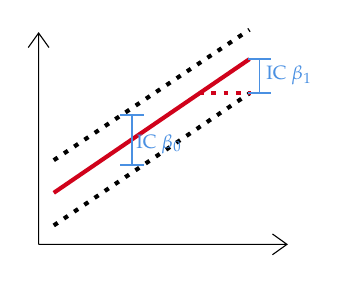
\begin{tikzpicture}[x=0.75pt,y=0.75pt,yscale=-1,xscale=1]
%uncomment if require: \path (0,300); %set diagram left start at 0, and has height of 300

%Shape: Axis 2D [id:dp4889594725047912] 
\draw  (91,151.4) -- (210.66,151.4)(91,49.57) -- (91,151.4) -- cycle (203.66,146.4) -- (210.66,151.4) -- (203.66,156.4) (86,56.57) -- (91,49.57) -- (96,56.57)  ;
%Straight Lines [id:da4199272602263775] 
\draw [line width=1.5]  [dash pattern={on 1.69pt off 2.76pt}]  (98.31,110.86) -- (192.59,48) ;


%Straight Lines [id:da6757115927785491] 
\draw [line width=1.5]  [dash pattern={on 1.69pt off 2.76pt}]  (98.31,142.29) -- (192.59,78.64) ;


%Straight Lines [id:da31286066421974423] 
\draw [color={rgb, 255:red, 208; green, 2; blue, 27 }  ,draw opacity=1 ][line width=1.5]    (98.31,126.57) -- (192.59,62.14) ;


%Straight Lines [id:da24370333728636973] 
\draw [color={rgb, 255:red, 208; green, 2; blue, 27 }  ,draw opacity=1 ][line width=1.5]  [dash pattern={on 1.69pt off 2.76pt}]  (168.24,78.64) -- (193.38,78.64) ;


%Straight Lines [id:da18662877299331004] 
\draw [color={rgb, 255:red, 74; green, 144; blue, 226 }  ,draw opacity=1 ]   (197.31,62.14) -- (197.31,78.64) ;
\draw [shift={(197.31,78.64)}, rotate = 270] [color={rgb, 255:red, 74; green, 144; blue, 226 }  ,draw opacity=1 ][line width=0.75]    (0,5.59) -- (0,-5.59)   ;
\draw [shift={(197.31,62.14)}, rotate = 270] [color={rgb, 255:red, 74; green, 144; blue, 226 }  ,draw opacity=1 ][line width=0.75]    (0,5.59) -- (0,-5.59)   ;
%Straight Lines [id:da8326995158666934] 
\draw [color={rgb, 255:red, 74; green, 144; blue, 226 }  ,draw opacity=1 ]   (136.02,88.86) -- (136.02,113.21) ;
\draw [shift={(136.02,113.21)}, rotate = 270] [color={rgb, 255:red, 74; green, 144; blue, 226 }  ,draw opacity=1 ][line width=0.75]    (0,5.59) -- (0,-5.59)   ;
\draw [shift={(136.02,88.86)}, rotate = 270] [color={rgb, 255:red, 74; green, 144; blue, 226 }  ,draw opacity=1 ][line width=0.75]    (0,5.59) -- (0,-5.59)   ;

% Text Node
\draw (149,103.16) node [scale=0.7,color={rgb, 255:red, 74; green, 144; blue, 226 }  ,opacity=1 ] [align=left] {IC $\beta_0$};
% Text Node
\draw (211.64,70.16) node [scale=0.7,color={rgb, 255:red, 74; green, 144; blue, 226 }  ,opacity=1 ] [align=left] {IC $\beta_1$};

\end{tikzpicture}

	\item \textbf{Process risk} pour $Y_0$. \\
		\textit{alias $\epsilon$} qui est la fluctuation des valeurs de la variable endogène $Y$ autour de sa moyenne.

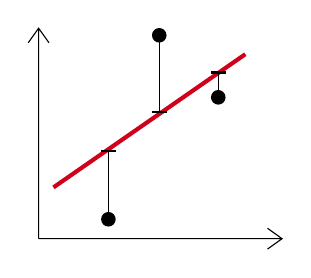
\begin{tikzpicture}[x=0.75pt,y=0.75pt,yscale=-1,xscale=1]
%uncomment if require: \path (0,300); %set diagram left start at 0, and has height of 300

%Shape: Axis 2D [id:dp4889594725047912] 
\draw  (91,151.4) -- (208.3,151.4)(91,50) -- (91,151.4) -- cycle (201.3,146.4) -- (208.3,151.4) -- (201.3,156.4) (86,57) -- (91,50) -- (96,57)  ;
%Straight Lines [id:da31286066421974423] 
\draw [color={rgb, 255:red, 208; green, 2; blue, 27 }  ,draw opacity=1 ][line width=1.5]    (98.16,126.68) -- (190.59,62.52) ;

%Straight Lines [id:da04588797245843623] 
\draw    (177.56,71.34) -- (177.56,83.29) ;
\draw [shift={(177.56,83.29)}, rotate = 90] [color={rgb, 255:red, 0; green, 0; blue, 0 }  ][fill={rgb, 255:red, 0; green, 0; blue, 0 }  ][line width=0.75]      (0, 0) circle [x radius= 3, y radius= 3]   ;
\draw [shift={(177.56,71.34)}, rotate = 270] [color={rgb, 255:red, 0; green, 0; blue, 0 }  ][line width=0.75]    (0,3.59) -- (0,-3.59)   ;
%Straight Lines [id:da010336451600581276] 
\draw    (149.13,90.26) -- (149.13,53.41) ;
\draw [shift={(149.13,53.41)}, rotate = 270] [color={rgb, 255:red, 0; green, 0; blue, 0 }  ][fill={rgb, 255:red, 0; green, 0; blue, 0 }  ][line width=0.75]      (0, 0) circle [x radius= 3, y radius= 3]   ;
\draw [shift={(149.13,90.26)}, rotate = 450] [color={rgb, 255:red, 0; green, 0; blue, 0 }  ][line width=0.75]    (0,3.59) -- (0,-3.59)   ;
%Straight Lines [id:da23452352145814448] 
\draw    (124.62,109.18) -- (124.62,142.04) ;
\draw [shift={(124.62,142.04)}, rotate = 90] [color={rgb, 255:red, 0; green, 0; blue, 0 }  ][fill={rgb, 255:red, 0; green, 0; blue, 0 }  ][line width=0.75]      (0, 0) circle [x radius= 3, y radius= 3]   ;
\draw [shift={(124.62,109.18)}, rotate = 270] [color={rgb, 255:red, 0; green, 0; blue, 0 }  ][line width=0.75]    (0,3.59) -- (0,-3.59)   ;

\end{tikzpicture}


\end{enumerate}

%\vfill\null

\subsubsection*{Intervalles de confiance de niveau $1 - \kappa$}
\begin{align*}
\esp{Y | x_0 } &\in \Bigg[ \widehat{Y}_0 \pm t_{(n - 2), \alpha/2} \sqrt{s^2 \bigg( \frac{1}{n} + \frac{(x_0 - \bar{x})^2}{S_{XX}} \bigg)} \Bigg] 
\end{align*}
On peut voir cet I.C. ci-dessous. \\
Plus $x^{*}$ s'éloigne de $\bar{x}$, plus l'incertitude augmente et l'I.C. est large.\\
On voit alors que les limites de l'intervalle sont des \textit{hyperboles} centrées en $(\bar{x}, \bar{Y})$.\\
De plus, on peut voir qu'on tient compte uniquement du \textbf{parameter risk} et non le \textbf{process risk}.

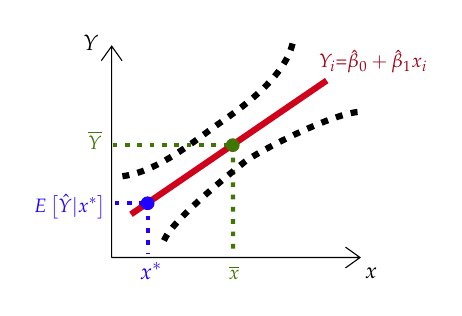
\begin{tikzpicture}[x=0.75pt,y=0.75pt,yscale=-1,xscale=1]
%uncomment if require: \path (0,300); %set diagram left start at 0, and has height of 300

%Shape: Axis 2D [id:dp870397431068519] 
\draw  (78,147.4) -- (197.66,147.4)(78,45.57) -- (78,147.4) -- cycle (190.66,142.4) -- (197.66,147.4) -- (190.66,152.4) (73,52.57) -- (78,45.57) -- (83,52.57)  ;
%Straight Lines [id:da5049173065442072] 
\draw [color={rgb, 255:red, 208; green, 2; blue, 27 }  ,draw opacity=1 ][line width=2.25]    (87.31,126.57) -- (181.59,62.14) ;


%Curve Lines [id:da7326433528773117] 
\draw [line width=2.25]  [dash pattern={on 2.53pt off 3.02pt}]  (83.17,108.22) .. controls (100.17,106.22) and (119.17,90.22) .. (129.17,83.22) .. controls (139.17,76.22) and (161.17,61.22) .. (165.17,44.22) ;


%Flowchart: Connector [id:dp2243219630944835] 
\draw  [color={rgb, 255:red, 65; green, 117; blue, 5 }  ,draw opacity=1 ][fill={rgb, 255:red, 65; green, 117; blue, 5 }  ,fill opacity=1 ] (133.27,93.26) .. controls (133.27,91.58) and (134.63,90.22) .. (136.31,90.22) .. controls (137.99,90.22) and (139.36,91.58) .. (139.36,93.26) .. controls (139.36,94.95) and (137.99,96.31) .. (136.31,96.31) .. controls (134.63,96.31) and (133.27,94.95) .. (133.27,93.26) -- cycle ;
%Flowchart: Connector [id:dp9119322800971501] 
\draw  [color={rgb, 255:red, 32; green, 0; blue, 255 }  ,draw opacity=1 ][fill={rgb, 255:red, 32; green, 0; blue, 255 }  ,fill opacity=1 ] (92.27,121.26) .. controls (92.27,119.58) and (93.63,118.22) .. (95.31,118.22) .. controls (96.99,118.22) and (98.36,119.58) .. (98.36,121.26) .. controls (98.36,122.95) and (96.99,124.31) .. (95.31,124.31) .. controls (93.63,124.31) and (92.27,122.95) .. (92.27,121.26) -- cycle ;
%Straight Lines [id:da06657275607687563] 
\draw [color={rgb, 255:red, 65; green, 117; blue, 5 }  ,draw opacity=1 ][line width=1.5]  [dash pattern={on 1.69pt off 2.76pt}]  (136.45,93.36) -- (136.5,145.89) ;


%Curve Lines [id:da5650856983111632] 
\draw [line width=2.25]  [dash pattern={on 2.53pt off 3.02pt}]  (103.17,139.22) .. controls (107.17,129.22) and (137.17,105.22) .. (142.17,101.22) .. controls (147.17,97.22) and (183.17,78.22) .. (197.17,77.22) ;


%Straight Lines [id:da7326669964019019] 
\draw [color={rgb, 255:red, 65; green, 117; blue, 5 }  ,draw opacity=1 ][line width=1.5]  [dash pattern={on 1.69pt off 2.76pt}]  (78.5,93.36) -- (136.45,93.36) ;


%Straight Lines [id:da3903502565018435] 
\draw [color={rgb, 255:red, 32; green, 0; blue, 255 }  ,draw opacity=1 ][line width=1.5]  [dash pattern={on 1.69pt off 2.76pt}]  (95.31,121.26) -- (95.31,145.89) ;


%Straight Lines [id:da01570604577282686] 
\draw [color={rgb, 255:red, 32; green, 0; blue, 255 }  ,draw opacity=1 ][line width=1.5]  [dash pattern={on 1.69pt off 2.76pt}]  (79.5,121.26) -- (95.31,121.26) ;




% Text Node
\draw (137,155) node [scale=0.7,color={rgb, 255:red, 65; green, 117; blue, 5 }  ,opacity=1 ] [align=left] {$\displaystyle \overline{x}$};
% Text Node
\draw (70,91) node [scale=0.7,color={rgb, 255:red, 65; green, 117; blue, 5 }  ,opacity=1 ] [align=left] {$\displaystyle \overline{Y}$};
% Text Node
\draw (97,154) node [scale=0.8,color={rgb, 255:red, 32; green, 0; blue, 255 }  ,opacity=1 ] [align=left] {$\displaystyle x^{*}$};
% Text Node
\draw (58,123) node [scale=0.7,color={rgb, 255:red, 32; green, 0; blue, 255 }  ,opacity=1 ] [align=left] {$\displaystyle E\left[\hat{Y} |x^{*}\right]$};
% Text Node
\draw (204,53) node [scale=0.7,color={rgb, 255:red, 157; green, 2; blue, 21 }  ,opacity=1 ] [align=left] {$\displaystyle Y_{i}$=$\displaystyle \hat{\beta }_{0} +\hat{\beta }_{1} x_{i}$};
% Text Node
\draw (68,44) node [scale=0.8] [align=left] {$\displaystyle Y$};
% Text Node
\draw (203,155) node [scale=0.8] [align=left] {$\displaystyle x$};


\end{tikzpicture}

L'I.C. pour la prévision tient compte du \textcolor{blue}{\textbf{process risk}} \textbf{\textit{en plus}} du \textbf{parameter risk}.

\begin{align*}
Y_0 &\in \Bigg[ \widehat{Y}_0 \pm t_{(n - 2), \alpha/2} \sqrt{s^2 \bigg( {\color{blue}1} + \frac{1}{n} + \frac{(x_0 - \bar{x})^2}{S_{XX}} \bigg)}\Bigg]
\end{align*}

\subsection*{Analyse de la variance (ANOVA)}
\textbf{Pour déterminer la proportion de la variabilité de $Y$ expliquée par le modèle}\\
\begin{tabular}{|g| *{4}{C|}}
\hline
\rowcolor{green!40!black} \color{white}{\text{Source}} & \color{white}{\text{dl}} & \color{white}{\text{SS}} & \color{white}{\text{MS}} & \color{white}{F} 
\\\hline
	Model & 
	p & 
	\thead{\sum_{i=1}^{n} (\hat{Y}_i - \bar{Y})^2 \\ \textbf{(SSR)}}  & \thead{SSR / dl_1 \\ (\textbf{MSR})} & \frac{MSR}{MSE} 
\\\hline
	Residual error & n - p' & \thead{\sum_{i=1}^{n} (Y_i - \hat{Y}_i)^2 \\ \textbf{(SSE)}} & \thead{SSE / dl_2 \\(\textbf{MSE} = s^2)} & \cellcolor{gray!30!white} 
\\\hline
	Total & n - 1 & \thead{\sum_{i=1}^{n} (Y_i - \bar{Y})^2 \\ \textbf{(SST)}} & \cellcolor{gray!30!white} & \cellcolor{gray!30!white} 
\\\hline
\end{tabular}
Où:
\begin{enumerate}
	\item[$p$: ] Nombre de variables explicatives dans le modèle.
	\item[$p$': ] Nombre de variables estimées dans le modèle.
\end{enumerate}  

\textbf{SSR}: Quantifie la variabilité des prévisions $\widehat{Y}_i$ expliquée par le modèle car elles ne sont pas tous égales à la moyenne $\bar{Y}_i$. 

\textbf{SSE}: Quantifie la variabilité des $Y_i - \widehat{Y}_i$ \textit{\textbf{pas}} expliquée par le modèle car il n'explique pas parfaitement $Y_i$.
%\\$\esp{MSR} = \sigma^{2} + \beta_{1}^{2}S_{XX}$\\
%$\esp{MSR} = \sigma^{2}$

\subsubsection*{Coefficient de détermination}
Représente la proportion de la variation de la variable endogène $Y$ qui est expliquée par le modèle.
\begin{align*}
R^2 = \frac{SSR}{SST} = 1 - \frac{SSE}{SST}
\end{align*}
%On a aussi la relation suivante avec $F_{obs}$ : 
%\begin{align*}
%F = \frac{R^2}{1 - R^2} \cdot \frac{n-p'}{p}
%\end{align*}

\subsubsection*{Test F de Fisher pour la validité globale de la régression}
On rejette $H_0 : \beta_1 =  \beta_2 = ... =  \beta_p = 0$ si 
\begin{align*}
F_{obs} &= \frac{MSR}{MSE} \geq F_{p, n-p'}(1 - \alpha) 
\end{align*}
%où $p$ est le nombre de variables explicatives dans le modèle (régression linéaire simple, $p=1$ et $p' = p+1$).\\
À noter qu'on peut réécrire $F_{\text{obs}} = \frac{1 - R^{2}}{R^{2}}$


\subsection*{Distribution d'un résidu $\varepsilon$}
\begin{tabular}{| >{\columncolor[gray]{.8}}c |c | c|}
\hline
$E[\widehat{\epsilon}_i]$ & $0$ & $\mathcal{H}_{1}$\\\hline
$V(\widehat{\epsilon}_i)$ & $\sigma^2(1 - h_{ii})$& $\mathcal{H}_{2}$ \\\hline
$Cov(\widehat{\epsilon}_i, \widehat{\epsilon}_j)$ & $-\sigma^2 \bigg( \frac{1}{n} + \frac{(x_i - \bar{x})(x_j - \bar{x})}{S_{xx}}\bigg)$ & $\mathcal{H}_{3}$ \\\hline
$\widehat{\epsilon}_i$ & $\sim \mathcal{N}(0, \sigma^2(1 - h_{ii}))$& $\mathcal{H}_{4}$ \\\hline
\end{tabular} \\
où $h_{ii} = \frac{1}{n} + \frac{(x_i - \bar{x})^2}{S_{XX}}$.\\
On peut interpréter $h_{ii}$ comme étant la \textit{"proportion"} de la variabilité du modèle \textit{$\sigma^{2}$} \textit{"expliquée"} par la $\text{i}^{\text{e}}$ observation. \\
Pour mieux le voir:
$h_{ii} = \frac{1}{n} + \frac{(x_i - \bar{x})^2}{\sum_{j = 1}^{n}(x_j - \bar{x})^2}$.\\
Donc, $h_{ii}$ est une des $n$ observations et $(x_{i} - \bar{x})^{2}$ est une des $n$ erreurs au carré; en multipliant par $\sigma^{2}$ on obtient la \textit{"proportion"} de la variabilité du résidu attribué au $\text{i}^{\text{e}}$ résidu $\hat\epsilon_{i}$.
%On peut aussi prouver que
%\begin{align*}
%\mathrm{Cov}(\hat{\varepsilon}_i, \hat{\varepsilon}_j) = - \sigma^2 \left( \frac{1}{n} + \frac{(x_i - \bar{x})(x_j - \bar{x})}{S_{XX}} \right)
%\end{align*}

\subsection*{Vérification des postulats}
%
%Les \textbf{résidus ordinaires} $\epsilon_{i} = Y_{i} - \hat{Y}_{i}$
%Si l'hypothèse
%\begin{enumerate}
%	\item[$\mathcal{H}_{1}$] est vérifié, $\esp{\hat{\epsilon_{i}}} = 0$.
%	\item[$\mathcal{H}_{2}$] est vérifié, $\text{V}(\hat{\epsilon_{i}}) = \sigma^2(1 - h_{ii})$.
%	\item[$\mathcal{H}_{3}$] est vraie, $\text{Cov}(\hat{\epsilon_{i}}, \hat{\epsilon_{j}}) = -h_{ij}\sigma^2$.
%	\item[$\mathcal{H}_{4}$] est vérifié, $\hat{\epsilon_{i}} \sim \mathcal{N}(0, \sigma^2(1 - h_{ii}))$.
%\end{enumerate}

Les résidus studentisés sont définis par
\begin{align*}
r_i &= \frac{\hat{\varepsilon}_i}{\sqrt{s^2(1 - h_{ii})}}
\end{align*}

\subsubsection*{Linéarité}
Utilise 3 types de graphiques \textit{(en nuage de points)}.
\begin{itemize}
\item graphique $Y_i | x_i$: On veut que l'allure de la relation ait l'air linéaire.

\tikzset{every picture/.style={line width=0.75pt}} %set default line width to 0.75pt        

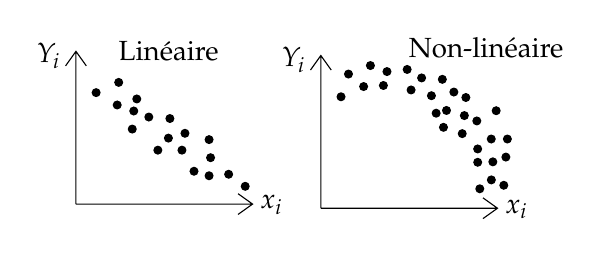
\begin{tikzpicture}[x=0.75pt,y=0.75pt,yscale=-1,xscale=1]
%uncomment if require: \path (0,300); %set diagram left start at 0, and has height of 300

%Shape: Axis 2D [id:dp47364438239602125] 
\draw  (38.32,89.58) -- (123.43,89.58)(38.32,16) -- (38.32,89.58) -- cycle (116.43,84.58) -- (123.43,89.58) -- (116.43,94.58) (33.32,23) -- (38.32,16) -- (43.32,23)  ;
%Flowchart: Connector [id:dp3277826883916124] 
\draw  [fill={rgb, 255:red, 0; green, 0; blue, 0 }  ,fill opacity=1 ] (63.57,53.45) .. controls (63.57,52.4) and (64.41,51.56) .. (65.46,51.56) .. controls (66.5,51.56) and (67.34,52.4) .. (67.34,53.45) .. controls (67.34,54.49) and (66.5,55.33) .. (65.46,55.33) .. controls (64.41,55.33) and (63.57,54.49) .. (63.57,53.45) -- cycle ;
%Flowchart: Connector [id:dp7058699867241285] 
\draw  [fill={rgb, 255:red, 0; green, 0; blue, 0 }  ,fill opacity=1 ] (93.32,73.76) .. controls (93.32,72.72) and (94.16,71.88) .. (95.21,71.88) .. controls (96.25,71.88) and (97.09,72.72) .. (97.09,73.76) .. controls (97.09,74.81) and (96.25,75.65) .. (95.21,75.65) .. controls (94.16,75.65) and (93.32,74.81) .. (93.32,73.76) -- cycle ;
%Flowchart: Connector [id:dp8404718863078824] 
\draw  [fill={rgb, 255:red, 0; green, 0; blue, 0 }  ,fill opacity=1 ] (100.58,58.53) .. controls (100.58,57.48) and (101.42,56.64) .. (102.46,56.64) .. controls (103.5,56.64) and (104.35,57.48) .. (104.35,58.53) .. controls (104.35,59.57) and (103.5,60.41) .. (102.46,60.41) .. controls (101.42,60.41) and (100.58,59.57) .. (100.58,58.53) -- cycle ;
%Flowchart: Connector [id:dp26963402638695944] 
\draw  [fill={rgb, 255:red, 0; green, 0; blue, 0 }  ,fill opacity=1 ] (71.55,47.64) .. controls (71.55,46.6) and (72.4,45.76) .. (73.44,45.76) .. controls (74.48,45.76) and (75.32,46.6) .. (75.32,47.64) .. controls (75.32,48.68) and (74.48,49.53) .. (73.44,49.53) .. controls (72.4,49.53) and (71.55,48.68) .. (71.55,47.64) -- cycle ;
%Flowchart: Connector [id:dp8003375971697122] 
\draw  [fill={rgb, 255:red, 0; green, 0; blue, 0 }  ,fill opacity=1 ] (64.29,44.74) .. controls (64.29,43.7) and (65.14,42.85) .. (66.18,42.85) .. controls (67.22,42.85) and (68.07,43.7) .. (68.07,44.74) .. controls (68.07,45.78) and (67.22,46.63) .. (66.18,46.63) .. controls (65.14,46.63) and (64.29,45.78) .. (64.29,44.74) -- cycle ;
%Flowchart: Connector [id:dp8404496157375017] 
\draw  [fill={rgb, 255:red, 0; green, 0; blue, 0 }  ,fill opacity=1 ] (87.51,63.61) .. controls (87.51,62.56) and (88.36,61.72) .. (89.4,61.72) .. controls (90.44,61.72) and (91.29,62.56) .. (91.29,63.61) .. controls (91.29,64.65) and (90.44,65.49) .. (89.4,65.49) .. controls (88.36,65.49) and (87.51,64.65) .. (87.51,63.61) -- cycle ;
%Flowchart: Connector [id:dp8480342341891878] 
\draw  [fill={rgb, 255:red, 0; green, 0; blue, 0 }  ,fill opacity=1 ] (75.9,63.61) .. controls (75.9,62.56) and (76.75,61.72) .. (77.79,61.72) .. controls (78.83,61.72) and (79.68,62.56) .. (79.68,63.61) .. controls (79.68,64.65) and (78.83,65.49) .. (77.79,65.49) .. controls (76.75,65.49) and (75.9,64.65) .. (75.9,63.61) -- cycle ;
%Flowchart: Connector [id:dp03818285836527546] 
\draw  [fill={rgb, 255:red, 0; green, 0; blue, 0 }  ,fill opacity=1 ] (80.98,57.8) .. controls (80.98,56.76) and (81.83,55.91) .. (82.87,55.91) .. controls (83.91,55.91) and (84.76,56.76) .. (84.76,57.8) .. controls (84.76,58.84) and (83.91,59.69) .. (82.87,59.69) .. controls (81.83,59.69) and (80.98,58.84) .. (80.98,57.8) -- cycle ;
%Flowchart: Connector [id:dp30311544112566113] 
\draw  [fill={rgb, 255:red, 0; green, 0; blue, 0 }  ,fill opacity=1 ] (117.99,81.02) .. controls (117.99,79.98) and (118.84,79.13) .. (119.88,79.13) .. controls (120.92,79.13) and (121.76,79.98) .. (121.76,81.02) .. controls (121.76,82.06) and (120.92,82.91) .. (119.88,82.91) .. controls (118.84,82.91) and (117.99,82.06) .. (117.99,81.02) -- cycle ;
%Flowchart: Connector [id:dp10052482685841602] 
\draw  [fill={rgb, 255:red, 0; green, 0; blue, 0 }  ,fill opacity=1 ] (100.58,75.94) .. controls (100.58,74.9) and (101.42,74.05) .. (102.46,74.05) .. controls (103.5,74.05) and (104.35,74.9) .. (104.35,75.94) .. controls (104.35,76.98) and (103.5,77.83) .. (102.46,77.83) .. controls (101.42,77.83) and (100.58,76.98) .. (100.58,75.94) -- cycle ;
%Flowchart: Connector [id:dp08087959913185516] 
\draw  [fill={rgb, 255:red, 0; green, 0; blue, 0 }  ,fill opacity=1 ] (110.01,75.22) .. controls (110.01,74.17) and (110.85,73.33) .. (111.9,73.33) .. controls (112.94,73.33) and (113.78,74.17) .. (113.78,75.22) .. controls (113.78,76.26) and (112.94,77.1) .. (111.9,77.1) .. controls (110.85,77.1) and (110.01,76.26) .. (110.01,75.22) -- cycle ;
%Flowchart: Connector [id:dp3959515580543951] 
\draw  [fill={rgb, 255:red, 0; green, 0; blue, 0 }  ,fill opacity=1 ] (101.3,67.23) .. controls (101.3,66.19) and (102.15,65.35) .. (103.19,65.35) .. controls (104.23,65.35) and (105.07,66.19) .. (105.07,67.23) .. controls (105.07,68.28) and (104.23,69.12) .. (103.19,69.12) .. controls (102.15,69.12) and (101.3,68.28) .. (101.3,67.23) -- cycle ;
%Flowchart: Connector [id:dp3611663792340556] 
\draw  [fill={rgb, 255:red, 0; green, 0; blue, 0 }  ,fill opacity=1 ] (56.31,41.84) .. controls (56.31,40.8) and (57.16,39.95) .. (58.2,39.95) .. controls (59.24,39.95) and (60.09,40.8) .. (60.09,41.84) .. controls (60.09,42.88) and (59.24,43.72) .. (58.2,43.72) .. controls (57.16,43.72) and (56.31,42.88) .. (56.31,41.84) -- cycle ;
%Flowchart: Connector [id:dp038389586369763196] 
\draw  [fill={rgb, 255:red, 0; green, 0; blue, 0 }  ,fill opacity=1 ] (65.75,38.93) .. controls (65.75,37.89) and (66.59,37.05) .. (67.63,37.05) .. controls (68.67,37.05) and (69.52,37.89) .. (69.52,38.93) .. controls (69.52,39.98) and (68.67,40.82) .. (67.63,40.82) .. controls (66.59,40.82) and (65.75,39.98) .. (65.75,38.93) -- cycle ;
%Flowchart: Connector [id:dp4866776658168612] 
\draw  [fill={rgb, 255:red, 0; green, 0; blue, 0 }  ,fill opacity=1 ] (57.04,30.95) .. controls (57.04,29.91) and (57.88,29.07) .. (58.92,29.07) .. controls (59.97,29.07) and (60.81,29.91) .. (60.81,30.95) .. controls (60.81,31.99) and (59.97,32.84) .. (58.92,32.84) .. controls (57.88,32.84) and (57.04,31.99) .. (57.04,30.95) -- cycle ;
%Flowchart: Connector [id:dp10201650082481928] 
\draw  [fill={rgb, 255:red, 0; green, 0; blue, 0 }  ,fill opacity=1 ] (81.71,48.37) .. controls (81.71,47.33) and (82.55,46.48) .. (83.6,46.48) .. controls (84.64,46.48) and (85.48,47.33) .. (85.48,48.37) .. controls (85.48,49.41) and (84.64,50.25) .. (83.6,50.25) .. controls (82.55,50.25) and (81.71,49.41) .. (81.71,48.37) -- cycle ;
%Flowchart: Connector [id:dp013575005320923594] 
\draw  [fill={rgb, 255:red, 0; green, 0; blue, 0 }  ,fill opacity=1 ] (88.97,55.48) .. controls (88.97,54.44) and (89.81,53.59) .. (90.85,53.59) .. controls (91.89,53.59) and (92.74,54.44) .. (92.74,55.48) .. controls (92.74,56.52) and (91.89,57.37) .. (90.85,57.37) .. controls (89.81,57.37) and (88.97,56.52) .. (88.97,55.48) -- cycle ;
%Flowchart: Connector [id:dp482963488799359] 
\draw  [fill={rgb, 255:red, 0; green, 0; blue, 0 }  ,fill opacity=1 ] (46.15,35.89) .. controls (46.15,34.84) and (47,34) .. (48.04,34) .. controls (49.08,34) and (49.93,34.84) .. (49.93,35.89) .. controls (49.93,36.93) and (49.08,37.77) .. (48.04,37.77) .. controls (47,37.77) and (46.15,36.93) .. (46.15,35.89) -- cycle ;

%Shape: Axis 2D [id:dp6020490257672775] 
\draw  (156.32,91.58) -- (241.43,91.58)(156.32,18) -- (156.32,91.58) -- cycle (234.43,86.58) -- (241.43,91.58) -- (234.43,96.58) (151.32,25) -- (156.32,18) -- (161.32,25)  ;
%Flowchart: Connector [id:dp8865449287034504] 
\draw  [fill={rgb, 255:red, 0; green, 0; blue, 0 }  ,fill opacity=1 ] (184.57,32.45) .. controls (184.57,31.4) and (185.41,30.56) .. (186.46,30.56) .. controls (187.5,30.56) and (188.34,31.4) .. (188.34,32.45) .. controls (188.34,33.49) and (187.5,34.33) .. (186.46,34.33) .. controls (185.41,34.33) and (184.57,33.49) .. (184.57,32.45) -- cycle ;
%Flowchart: Connector [id:dp09108500914974971] 
\draw  [fill={rgb, 255:red, 0; green, 0; blue, 0 }  ,fill opacity=1 ] (230.01,69.44) .. controls (230.01,68.4) and (230.85,67.56) .. (231.9,67.56) .. controls (232.94,67.56) and (233.78,68.4) .. (233.78,69.44) .. controls (233.78,70.48) and (232.94,71.33) .. (231.9,71.33) .. controls (230.85,71.33) and (230.01,70.48) .. (230.01,69.44) -- cycle ;
%Flowchart: Connector [id:dp3812423442661901] 
\draw  [fill={rgb, 255:red, 0; green, 0; blue, 0 }  ,fill opacity=1 ] (229.58,49.53) .. controls (229.58,48.48) and (230.42,47.64) .. (231.46,47.64) .. controls (232.5,47.64) and (233.35,48.48) .. (233.35,49.53) .. controls (233.35,50.57) and (232.5,51.41) .. (231.46,51.41) .. controls (230.42,51.41) and (229.58,50.57) .. (229.58,49.53) -- cycle ;
%Flowchart: Connector [id:dp32906760413195557] 
\draw  [fill={rgb, 255:red, 0; green, 0; blue, 0 }  ,fill opacity=1 ] (222.55,55.64) .. controls (222.55,54.6) and (223.4,53.76) .. (224.44,53.76) .. controls (225.48,53.76) and (226.32,54.6) .. (226.32,55.64) .. controls (226.32,56.68) and (225.48,57.53) .. (224.44,57.53) .. controls (223.4,57.53) and (222.55,56.68) .. (222.55,55.64) -- cycle ;
%Flowchart: Connector [id:dp8034942113246071] 
\draw  [fill={rgb, 255:red, 0; green, 0; blue, 0 }  ,fill opacity=1 ] (186.29,25.74) .. controls (186.29,24.7) and (187.14,23.85) .. (188.18,23.85) .. controls (189.22,23.85) and (190.07,24.7) .. (190.07,25.74) .. controls (190.07,26.78) and (189.22,27.63) .. (188.18,27.63) .. controls (187.14,27.63) and (186.29,26.78) .. (186.29,25.74) -- cycle ;
%Flowchart: Connector [id:dp8644196115326095] 
\draw  [fill={rgb, 255:red, 0; green, 0; blue, 0 }  ,fill opacity=1 ] (213.51,52.61) .. controls (213.51,51.56) and (214.36,50.72) .. (215.4,50.72) .. controls (216.44,50.72) and (217.29,51.56) .. (217.29,52.61) .. controls (217.29,53.65) and (216.44,54.49) .. (215.4,54.49) .. controls (214.36,54.49) and (213.51,53.65) .. (213.51,52.61) -- cycle ;
%Flowchart: Connector [id:dp5120708439140604] 
\draw  [fill={rgb, 255:red, 0; green, 0; blue, 0 }  ,fill opacity=1 ] (238.9,44.61) .. controls (238.9,43.56) and (239.75,42.72) .. (240.79,42.72) .. controls (241.83,42.72) and (242.68,43.56) .. (242.68,44.61) .. controls (242.68,45.65) and (241.83,46.49) .. (240.79,46.49) .. controls (239.75,46.49) and (238.9,45.65) .. (238.9,44.61) -- cycle ;
%Flowchart: Connector [id:dp8543661259647852] 
\draw  [fill={rgb, 255:red, 0; green, 0; blue, 0 }  ,fill opacity=1 ] (209.98,45.8) .. controls (209.98,44.76) and (210.83,43.91) .. (211.87,43.91) .. controls (212.91,43.91) and (213.76,44.76) .. (213.76,45.8) .. controls (213.76,46.84) and (212.91,47.69) .. (211.87,47.69) .. controls (210.83,47.69) and (209.98,46.84) .. (209.98,45.8) -- cycle ;
%Flowchart: Connector [id:dp18657820969215866] 
\draw  [fill={rgb, 255:red, 0; green, 0; blue, 0 }  ,fill opacity=1 ] (229.99,63.02) .. controls (229.99,61.98) and (230.84,61.13) .. (231.88,61.13) .. controls (232.92,61.13) and (233.76,61.98) .. (233.76,63.02) .. controls (233.76,64.06) and (232.92,64.91) .. (231.88,64.91) .. controls (230.84,64.91) and (229.99,64.06) .. (229.99,63.02) -- cycle ;
%Flowchart: Connector [id:dp4309077985738581] 
\draw  [fill={rgb, 255:red, 0; green, 0; blue, 0 }  ,fill opacity=1 ] (223.58,46.94) .. controls (223.58,45.9) and (224.42,45.05) .. (225.46,45.05) .. controls (226.5,45.05) and (227.35,45.9) .. (227.35,46.94) .. controls (227.35,47.98) and (226.5,48.83) .. (225.46,48.83) .. controls (224.42,48.83) and (223.58,47.98) .. (223.58,46.94) -- cycle ;
%Flowchart: Connector [id:dp572335103076985] 
\draw  [fill={rgb, 255:red, 0; green, 0; blue, 0 }  ,fill opacity=1 ] (231.01,82.22) .. controls (231.01,81.17) and (231.85,80.33) .. (232.9,80.33) .. controls (233.94,80.33) and (234.78,81.17) .. (234.78,82.22) .. controls (234.78,83.26) and (233.94,84.1) .. (232.9,84.1) .. controls (231.85,84.1) and (231.01,83.26) .. (231.01,82.22) -- cycle ;
%Flowchart: Connector [id:dp029484150595288305] 
\draw  [fill={rgb, 255:red, 0; green, 0; blue, 0 }  ,fill opacity=1 ] (224.3,38.23) .. controls (224.3,37.19) and (225.15,36.35) .. (226.19,36.35) .. controls (227.23,36.35) and (228.07,37.19) .. (228.07,38.23) .. controls (228.07,39.28) and (227.23,40.12) .. (226.19,40.12) .. controls (225.15,40.12) and (224.3,39.28) .. (224.3,38.23) -- cycle ;
%Flowchart: Connector [id:dp7665816923657789] 
\draw  [fill={rgb, 255:red, 0; green, 0; blue, 0 }  ,fill opacity=1 ] (178.31,22.84) .. controls (178.31,21.8) and (179.16,20.95) .. (180.2,20.95) .. controls (181.24,20.95) and (182.09,21.8) .. (182.09,22.84) .. controls (182.09,23.88) and (181.24,24.72) .. (180.2,24.72) .. controls (179.16,24.72) and (178.31,23.88) .. (178.31,22.84) -- cycle ;
%Flowchart: Connector [id:dp19063151424370095] 
\draw  [fill={rgb, 255:red, 0; green, 0; blue, 0 }  ,fill opacity=1 ] (167.75,26.93) .. controls (167.75,25.89) and (168.59,25.05) .. (169.63,25.05) .. controls (170.67,25.05) and (171.52,25.89) .. (171.52,26.93) .. controls (171.52,27.98) and (170.67,28.82) .. (169.63,28.82) .. controls (168.59,28.82) and (167.75,27.98) .. (167.75,26.93) -- cycle ;
%Flowchart: Connector [id:dp3451083678311162] 
\draw  [fill={rgb, 255:red, 0; green, 0; blue, 0 }  ,fill opacity=1 ] (175.04,32.95) .. controls (175.04,31.91) and (175.88,31.07) .. (176.92,31.07) .. controls (177.97,31.07) and (178.81,31.91) .. (178.81,32.95) .. controls (178.81,33.99) and (177.97,34.84) .. (176.92,34.84) .. controls (175.88,34.84) and (175.04,33.99) .. (175.04,32.95) -- cycle ;
%Flowchart: Connector [id:dp7953283353975327] 
\draw  [fill={rgb, 255:red, 0; green, 0; blue, 0 }  ,fill opacity=1 ] (207.71,37.37) .. controls (207.71,36.33) and (208.55,35.48) .. (209.6,35.48) .. controls (210.64,35.48) and (211.48,36.33) .. (211.48,37.37) .. controls (211.48,38.41) and (210.64,39.25) .. (209.6,39.25) .. controls (208.55,39.25) and (207.71,38.41) .. (207.71,37.37) -- cycle ;
%Flowchart: Connector [id:dp10533255767401872] 
\draw  [fill={rgb, 255:red, 0; green, 0; blue, 0 }  ,fill opacity=1 ] (214.97,44.48) .. controls (214.97,43.44) and (215.81,42.59) .. (216.85,42.59) .. controls (217.89,42.59) and (218.74,43.44) .. (218.74,44.48) .. controls (218.74,45.52) and (217.89,46.37) .. (216.85,46.37) .. controls (215.81,46.37) and (214.97,45.52) .. (214.97,44.48) -- cycle ;
%Flowchart: Connector [id:dp32785171387479206] 
\draw  [fill={rgb, 255:red, 0; green, 0; blue, 0 }  ,fill opacity=1 ] (164.15,37.89) .. controls (164.15,36.84) and (165,36) .. (166.04,36) .. controls (167.08,36) and (167.93,36.84) .. (167.93,37.89) .. controls (167.93,38.93) and (167.08,39.77) .. (166.04,39.77) .. controls (165,39.77) and (164.15,38.93) .. (164.15,37.89) -- cycle ;
%Flowchart: Connector [id:dp05920464452564467] 
\draw  [fill={rgb, 255:red, 0; green, 0; blue, 0 }  ,fill opacity=1 ] (196.02,24.72) .. controls (196.02,23.68) and (196.86,22.83) .. (197.9,22.83) .. controls (198.95,22.83) and (199.79,23.68) .. (199.79,24.72) .. controls (199.79,25.76) and (198.95,26.61) .. (197.9,26.61) .. controls (196.86,26.61) and (196.02,25.76) .. (196.02,24.72) -- cycle ;
%Flowchart: Connector [id:dp09832977485823213] 
\draw  [fill={rgb, 255:red, 0; green, 0; blue, 0 }  ,fill opacity=1 ] (218.51,35.61) .. controls (218.51,34.56) and (219.36,33.72) .. (220.4,33.72) .. controls (221.44,33.72) and (222.29,34.56) .. (222.29,35.61) .. controls (222.29,36.65) and (221.44,37.49) .. (220.4,37.49) .. controls (219.36,37.49) and (218.51,36.65) .. (218.51,35.61) -- cycle ;
%Flowchart: Connector [id:dp719206652650972] 
\draw  [fill={rgb, 255:red, 0; green, 0; blue, 0 }  ,fill opacity=1 ] (197.9,34.61) .. controls (197.9,33.56) and (198.75,32.72) .. (199.79,32.72) .. controls (200.83,32.72) and (201.68,33.56) .. (201.68,34.61) .. controls (201.68,35.65) and (200.83,36.49) .. (199.79,36.49) .. controls (198.75,36.49) and (197.9,35.65) .. (197.9,34.61) -- cycle ;
%Flowchart: Connector [id:dp6431120660042795] 
\draw  [fill={rgb, 255:red, 0; green, 0; blue, 0 }  ,fill opacity=1 ] (202.98,28.8) .. controls (202.98,27.76) and (203.83,26.91) .. (204.87,26.91) .. controls (205.91,26.91) and (206.76,27.76) .. (206.76,28.8) .. controls (206.76,29.84) and (205.91,30.69) .. (204.87,30.69) .. controls (203.83,30.69) and (202.98,29.84) .. (202.98,28.8) -- cycle ;
%Flowchart: Connector [id:dp032740006628465546] 
\draw  [fill={rgb, 255:red, 0; green, 0; blue, 0 }  ,fill opacity=1 ] (212.97,29.48) .. controls (212.97,28.44) and (213.81,27.59) .. (214.85,27.59) .. controls (215.89,27.59) and (216.74,28.44) .. (216.74,29.48) .. controls (216.74,30.52) and (215.89,31.37) .. (214.85,31.37) .. controls (213.81,31.37) and (212.97,30.52) .. (212.97,29.48) -- cycle ;
%Flowchart: Connector [id:dp4393751981985121] 
\draw  [fill={rgb, 255:red, 0; green, 0; blue, 0 }  ,fill opacity=1 ] (236.53,58.23) .. controls (236.53,57.19) and (237.37,56.35) .. (238.41,56.35) .. controls (239.46,56.35) and (240.3,57.19) .. (240.3,58.23) .. controls (240.3,59.28) and (239.46,60.12) .. (238.41,60.12) .. controls (237.37,60.12) and (236.53,59.28) .. (236.53,58.23) -- cycle ;
%Flowchart: Connector [id:dp84909742390326] 
\draw  [fill={rgb, 255:red, 0; green, 0; blue, 0 }  ,fill opacity=1 ] (243.58,66.94) .. controls (243.58,65.9) and (244.42,65.05) .. (245.46,65.05) .. controls (246.5,65.05) and (247.35,65.9) .. (247.35,66.94) .. controls (247.35,67.98) and (246.5,68.83) .. (245.46,68.83) .. controls (244.42,68.83) and (243.58,67.98) .. (243.58,66.94) -- cycle ;
%Flowchart: Connector [id:dp9121722984701972] 
\draw  [fill={rgb, 255:red, 0; green, 0; blue, 0 }  ,fill opacity=1 ] (244.3,58.23) .. controls (244.3,57.19) and (245.15,56.35) .. (246.19,56.35) .. controls (247.23,56.35) and (248.07,57.19) .. (248.07,58.23) .. controls (248.07,59.28) and (247.23,60.12) .. (246.19,60.12) .. controls (245.15,60.12) and (244.3,59.28) .. (244.3,58.23) -- cycle ;
%Flowchart: Connector [id:dp5226023884972613] 
\draw  [fill={rgb, 255:red, 0; green, 0; blue, 0 }  ,fill opacity=1 ] (242.58,80.53) .. controls (242.58,79.48) and (243.42,78.64) .. (244.46,78.64) .. controls (245.5,78.64) and (246.35,79.48) .. (246.35,80.53) .. controls (246.35,81.57) and (245.5,82.41) .. (244.46,82.41) .. controls (243.42,82.41) and (242.58,81.57) .. (242.58,80.53) -- cycle ;
%Flowchart: Connector [id:dp5466788756165353] 
\draw  [fill={rgb, 255:red, 0; green, 0; blue, 0 }  ,fill opacity=1 ] (236.58,77.94) .. controls (236.58,76.9) and (237.42,76.05) .. (238.46,76.05) .. controls (239.5,76.05) and (240.35,76.9) .. (240.35,77.94) .. controls (240.35,78.98) and (239.5,79.83) .. (238.46,79.83) .. controls (237.42,79.83) and (236.58,78.98) .. (236.58,77.94) -- cycle ;
%Flowchart: Connector [id:dp05512702472089992] 
\draw  [fill={rgb, 255:red, 0; green, 0; blue, 0 }  ,fill opacity=1 ] (237.3,69.23) .. controls (237.3,68.19) and (238.15,67.35) .. (239.19,67.35) .. controls (240.23,67.35) and (241.07,68.19) .. (241.07,69.23) .. controls (241.07,70.28) and (240.23,71.12) .. (239.19,71.12) .. controls (238.15,71.12) and (237.3,70.28) .. (237.3,69.23) -- cycle ;

% Text Node
\draw (25.26,18.18) node  [align=left] {$\displaystyle Y_{i}$};
% Text Node
\draw (132.65,90.02) node  [align=left] {$\displaystyle x_{i}$};
% Text Node
\draw (250.65,92.02) node  [align=left] {$\displaystyle x_{i}$};
% Text Node
\draw (143.26,20.18) node  [align=left] {$\displaystyle Y_{i}$};
% Text Node
\draw (83,16) node  [align=left] {Linéaire};
% Text Node
\draw (236,14) node  [align=left] {Non-linéaire};


\end{tikzpicture}

\item graphique $\hat{\varepsilon}_i | \hat{Y}_i$: On veut que les points soient centrés verticalement en 0.\\
Il ne devrait pas avoir de tendances discernables du nuage de points \textit{(il devrait avoir l'air aléatoire)}.


\tikzset{every picture/.style={line width=0.75pt}} %set default line width to 0.75pt        

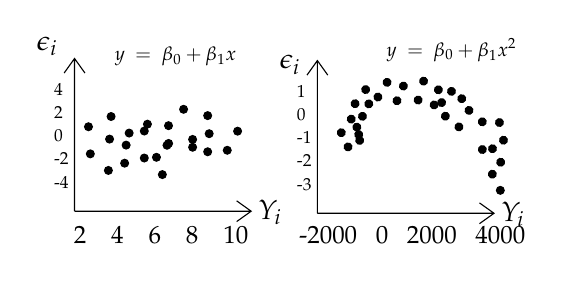
\begin{tikzpicture}[x=0.75pt,y=0.75pt,yscale=-1,xscale=1]
%uncomment if require: \path (0,113.19999694824219); %set diagram left start at 0, and has height of 113.19999694824219

%Shape: Axis 2D [id:dp7287261441525803] 
\draw  (39.32,90.58) -- (124.43,90.58)(39.32,17) -- (39.32,90.58) -- cycle (117.43,85.58) -- (124.43,90.58) -- (117.43,95.58) (34.32,24) -- (39.32,17) -- (44.32,24)  ;
%Flowchart: Connector [id:dp36309359457930324] 
\draw  [fill={rgb, 255:red, 0; green, 0; blue, 0 }  ,fill opacity=1 ] (61.57,67.45) .. controls (61.57,66.4) and (62.41,65.56) .. (63.46,65.56) .. controls (64.5,65.56) and (65.34,66.4) .. (65.34,67.45) .. controls (65.34,68.49) and (64.5,69.33) .. (63.46,69.33) .. controls (62.41,69.33) and (61.57,68.49) .. (61.57,67.45) -- cycle ;
%Flowchart: Connector [id:dp6736526834039009] 
\draw  [fill={rgb, 255:red, 0; green, 0; blue, 0 }  ,fill opacity=1 ] (94.32,59.76) .. controls (94.32,58.72) and (95.16,57.88) .. (96.21,57.88) .. controls (97.25,57.88) and (98.09,58.72) .. (98.09,59.76) .. controls (98.09,60.81) and (97.25,61.65) .. (96.21,61.65) .. controls (95.16,61.65) and (94.32,60.81) .. (94.32,59.76) -- cycle ;
%Flowchart: Connector [id:dp046828506273816295] 
\draw  [fill={rgb, 255:red, 0; green, 0; blue, 0 }  ,fill opacity=1 ] (101.58,44.53) .. controls (101.58,43.48) and (102.42,42.64) .. (103.46,42.64) .. controls (104.5,42.64) and (105.35,43.48) .. (105.35,44.53) .. controls (105.35,45.57) and (104.5,46.41) .. (103.46,46.41) .. controls (102.42,46.41) and (101.58,45.57) .. (101.58,44.53) -- cycle ;
%Flowchart: Connector [id:dp8986151523486408] 
\draw  [fill={rgb, 255:red, 0; green, 0; blue, 0 }  ,fill opacity=1 ] (72.55,48.64) .. controls (72.55,47.6) and (73.4,46.76) .. (74.44,46.76) .. controls (75.48,46.76) and (76.32,47.6) .. (76.32,48.64) .. controls (76.32,49.68) and (75.48,50.53) .. (74.44,50.53) .. controls (73.4,50.53) and (72.55,49.68) .. (72.55,48.64) -- cycle ;
%Flowchart: Connector [id:dp7572329250054246] 
\draw  [fill={rgb, 255:red, 0; green, 0; blue, 0 }  ,fill opacity=1 ] (62.29,58.74) .. controls (62.29,57.7) and (63.14,56.85) .. (64.18,56.85) .. controls (65.22,56.85) and (66.07,57.7) .. (66.07,58.74) .. controls (66.07,59.78) and (65.22,60.63) .. (64.18,60.63) .. controls (63.14,60.63) and (62.29,59.78) .. (62.29,58.74) -- cycle ;
%Flowchart: Connector [id:dp47552983389665626] 
\draw  [fill={rgb, 255:red, 0; green, 0; blue, 0 }  ,fill opacity=1 ] (94.32,55.99) .. controls (94.32,54.95) and (95.16,54.1) .. (96.21,54.1) .. controls (97.25,54.1) and (98.09,54.95) .. (98.09,55.99) .. controls (98.09,57.03) and (97.25,57.88) .. (96.21,57.88) .. controls (95.16,57.88) and (94.32,57.03) .. (94.32,55.99) -- cycle ;
%Flowchart: Connector [id:dp8844255628350515] 
\draw  [fill={rgb, 255:red, 0; green, 0; blue, 0 }  ,fill opacity=1 ] (76.9,64.61) .. controls (76.9,63.56) and (77.75,62.72) .. (78.79,62.72) .. controls (79.83,62.72) and (80.68,63.56) .. (80.68,64.61) .. controls (80.68,65.65) and (79.83,66.49) .. (78.79,66.49) .. controls (77.75,66.49) and (76.9,65.65) .. (76.9,64.61) -- cycle ;
%Flowchart: Connector [id:dp6795761837513346] 
\draw  [fill={rgb, 255:red, 0; green, 0; blue, 0 }  ,fill opacity=1 ] (81.98,58.8) .. controls (81.98,57.76) and (82.83,56.91) .. (83.87,56.91) .. controls (84.91,56.91) and (85.76,57.76) .. (85.76,58.8) .. controls (85.76,59.84) and (84.91,60.69) .. (83.87,60.69) .. controls (82.83,60.69) and (81.98,59.84) .. (81.98,58.8) -- cycle ;
%Flowchart: Connector [id:dp0163019056153193] 
\draw  [fill={rgb, 255:red, 0; green, 0; blue, 0 }  ,fill opacity=1 ] (115.99,52.02) .. controls (115.99,50.98) and (116.84,50.13) .. (117.88,50.13) .. controls (118.92,50.13) and (119.76,50.98) .. (119.76,52.02) .. controls (119.76,53.06) and (118.92,53.91) .. (117.88,53.91) .. controls (116.84,53.91) and (115.99,53.06) .. (115.99,52.02) -- cycle ;
%Flowchart: Connector [id:dp41849658031091197] 
\draw  [fill={rgb, 255:red, 0; green, 0; blue, 0 }  ,fill opacity=1 ] (101.58,61.94) .. controls (101.58,60.9) and (102.42,60.05) .. (103.46,60.05) .. controls (104.5,60.05) and (105.35,60.9) .. (105.35,61.94) .. controls (105.35,62.98) and (104.5,63.83) .. (103.46,63.83) .. controls (102.42,63.83) and (101.58,62.98) .. (101.58,61.94) -- cycle ;
%Flowchart: Connector [id:dp6579227183890666] 
\draw  [fill={rgb, 255:red, 0; green, 0; blue, 0 }  ,fill opacity=1 ] (111.01,61.22) .. controls (111.01,60.17) and (111.85,59.33) .. (112.9,59.33) .. controls (113.94,59.33) and (114.78,60.17) .. (114.78,61.22) .. controls (114.78,62.26) and (113.94,63.1) .. (112.9,63.1) .. controls (111.85,63.1) and (111.01,62.26) .. (111.01,61.22) -- cycle ;
%Flowchart: Connector [id:dp384654239387336] 
\draw  [fill={rgb, 255:red, 0; green, 0; blue, 0 }  ,fill opacity=1 ] (102.3,53.23) .. controls (102.3,52.19) and (103.15,51.35) .. (104.19,51.35) .. controls (105.23,51.35) and (106.07,52.19) .. (106.07,53.23) .. controls (106.07,54.28) and (105.23,55.12) .. (104.19,55.12) .. controls (103.15,55.12) and (102.3,54.28) .. (102.3,53.23) -- cycle ;
%Flowchart: Connector [id:dp13101684098199962] 
\draw  [fill={rgb, 255:red, 0; green, 0; blue, 0 }  ,fill opacity=1 ] (54.31,55.84) .. controls (54.31,54.8) and (55.16,53.95) .. (56.2,53.95) .. controls (57.24,53.95) and (58.09,54.8) .. (58.09,55.84) .. controls (58.09,56.88) and (57.24,57.72) .. (56.2,57.72) .. controls (55.16,57.72) and (54.31,56.88) .. (54.31,55.84) -- cycle ;
%Flowchart: Connector [id:dp0014583187536478803] 
\draw  [fill={rgb, 255:red, 0; green, 0; blue, 0 }  ,fill opacity=1 ] (63.75,52.93) .. controls (63.75,51.89) and (64.59,51.05) .. (65.63,51.05) .. controls (66.67,51.05) and (67.52,51.89) .. (67.52,52.93) .. controls (67.52,53.98) and (66.67,54.82) .. (65.63,54.82) .. controls (64.59,54.82) and (63.75,53.98) .. (63.75,52.93) -- cycle ;
%Flowchart: Connector [id:dp4488910824281127] 
\draw  [fill={rgb, 255:red, 0; green, 0; blue, 0 }  ,fill opacity=1 ] (55.04,44.95) .. controls (55.04,43.91) and (55.88,43.07) .. (56.92,43.07) .. controls (57.97,43.07) and (58.81,43.91) .. (58.81,44.95) .. controls (58.81,45.99) and (57.97,46.84) .. (56.92,46.84) .. controls (55.88,46.84) and (55.04,45.99) .. (55.04,44.95) -- cycle ;
%Flowchart: Connector [id:dp20952800246332903] 
\draw  [fill={rgb, 255:red, 0; green, 0; blue, 0 }  ,fill opacity=1 ] (82.71,49.37) .. controls (82.71,48.33) and (83.55,47.48) .. (84.6,47.48) .. controls (85.64,47.48) and (86.48,48.33) .. (86.48,49.37) .. controls (86.48,50.41) and (85.64,51.25) .. (84.6,51.25) .. controls (83.55,51.25) and (82.71,50.41) .. (82.71,49.37) -- cycle ;
%Flowchart: Connector [id:dp7603231100029897] 
\draw  [fill={rgb, 255:red, 0; green, 0; blue, 0 }  ,fill opacity=1 ] (89.97,41.48) .. controls (89.97,40.44) and (90.81,39.59) .. (91.85,39.59) .. controls (92.89,39.59) and (93.74,40.44) .. (93.74,41.48) .. controls (93.74,42.52) and (92.89,43.37) .. (91.85,43.37) .. controls (90.81,43.37) and (89.97,42.52) .. (89.97,41.48) -- cycle ;
%Flowchart: Connector [id:dp07674120582326771] 
\draw  [fill={rgb, 255:red, 0; green, 0; blue, 0 }  ,fill opacity=1 ] (44.15,49.89) .. controls (44.15,48.84) and (45,48) .. (46.04,48) .. controls (47.08,48) and (47.93,48.84) .. (47.93,49.89) .. controls (47.93,50.93) and (47.08,51.77) .. (46.04,51.77) .. controls (45,51.77) and (44.15,50.93) .. (44.15,49.89) -- cycle ;
%Shape: Axis 2D [id:dp1359977507444563] 
\draw  (156.32,91.58) -- (241.43,91.58)(156.32,18) -- (156.32,91.58) -- cycle (234.43,86.58) -- (241.43,91.58) -- (234.43,96.58) (151.32,25) -- (156.32,18) -- (161.32,25)  ;
%Flowchart: Connector [id:dp009438717531352614] 
\draw  [fill={rgb, 255:red, 0; green, 0; blue, 0 }  ,fill opacity=1 ] (184.94,37.38) .. controls (183.95,37.08) and (183.38,36.02) .. (183.69,35.03) .. controls (183.99,34.03) and (185.04,33.46) .. (186.04,33.77) .. controls (187.04,34.07) and (187.6,35.12) .. (187.3,36.12) .. controls (186.99,37.12) and (185.94,37.68) .. (184.94,37.38) -- cycle ;
%Flowchart: Connector [id:dp8155325578927763] 
\draw  [fill={rgb, 255:red, 0; green, 0; blue, 0 }  ,fill opacity=1 ] (234,61.44) .. controls (233.69,60.44) and (234.24,59.38) .. (235.23,59.07) .. controls (236.22,58.75) and (237.28,59.3) .. (237.6,60.3) .. controls (237.91,61.29) and (237.36,62.35) .. (236.37,62.66) .. controls (235.38,62.98) and (234.32,62.43) .. (234,61.44) -- cycle ;
%Flowchart: Connector [id:dp015226938430133785] 
\draw  [fill={rgb, 255:red, 0; green, 0; blue, 0 }  ,fill opacity=1 ] (227.57,42.58) .. controls (227.26,41.59) and (227.81,40.53) .. (228.8,40.21) .. controls (229.8,39.9) and (230.86,40.45) .. (231.17,41.44) .. controls (231.49,42.43) and (230.94,43.49) .. (229.94,43.81) .. controls (228.95,44.12) and (227.89,43.57) .. (227.57,42.58) -- cycle ;
%Flowchart: Connector [id:dp3684822979701521] 
\draw  [fill={rgb, 255:red, 0; green, 0; blue, 0 }  ,fill opacity=1 ] (222.72,50.53) .. controls (222.41,49.54) and (222.96,48.48) .. (223.95,48.16) .. controls (224.95,47.85) and (226.01,48.4) .. (226.32,49.39) .. controls (226.64,50.39) and (226.09,51.45) .. (225.09,51.76) .. controls (224.1,52.08) and (223.04,51.53) .. (222.72,50.53) -- cycle ;
%Flowchart: Connector [id:dp4848033346589644] 
\draw  [fill={rgb, 255:red, 0; green, 0; blue, 0 }  ,fill opacity=1 ] (179.03,33.78) .. controls (178.03,33.48) and (177.47,32.43) .. (177.77,31.43) .. controls (178.07,30.43) and (179.12,29.87) .. (180.12,30.17) .. controls (181.12,30.47) and (181.68,31.53) .. (181.38,32.52) .. controls (181.08,33.52) and (180.02,34.08) .. (179.03,33.78) -- cycle ;
%Flowchart: Connector [id:dp07082238067540914] 
\draw  [fill={rgb, 255:red, 0; green, 0; blue, 0 }  ,fill opacity=1 ] (216.19,45.37) .. controls (215.88,44.37) and (216.43,43.31) .. (217.42,43) .. controls (218.41,42.68) and (219.48,43.23) .. (219.79,44.23) .. controls (220.1,45.22) and (219.55,46.28) .. (218.56,46.6) .. controls (217.57,46.91) and (216.51,46.36) .. (216.19,45.37) -- cycle ;
%Flowchart: Connector [id:dp48115254429580334] 
\draw  [fill={rgb, 255:red, 0; green, 0; blue, 0 }  ,fill opacity=1 ] (233.98,48.07) .. controls (233.67,47.08) and (234.22,46.02) .. (235.21,45.7) .. controls (236.2,45.39) and (237.26,45.94) .. (237.58,46.93) .. controls (237.89,47.93) and (237.34,48.99) .. (236.35,49.3) .. controls (235.36,49.62) and (234.3,49.06) .. (233.98,48.07) -- cycle ;
%Flowchart: Connector [id:dp834309427345514] 
\draw  [fill={rgb, 255:red, 0; green, 0; blue, 0 }  ,fill opacity=1 ] (210.77,39.95) .. controls (210.46,38.95) and (211.01,37.89) .. (212,37.58) .. controls (212.99,37.26) and (214.05,37.81) .. (214.37,38.81) .. controls (214.68,39.8) and (214.13,40.86) .. (213.14,41.17) .. controls (212.15,41.49) and (211.09,40.94) .. (210.77,39.95) -- cycle ;
%Flowchart: Connector [id:dp41445073700876156] 
\draw  [fill={rgb, 255:red, 0; green, 0; blue, 0 }  ,fill opacity=1 ] (166.04,53.32) .. controls (165.73,52.33) and (166.28,51.27) .. (167.27,50.95) .. controls (168.27,50.64) and (169.33,51.19) .. (169.64,52.18) .. controls (169.96,53.17) and (169.41,54.23) .. (168.41,54.55) .. controls (167.42,54.86) and (166.36,54.31) .. (166.04,53.32) -- cycle ;
%Flowchart: Connector [id:dp6467856290398479] 
\draw  [fill={rgb, 255:red, 0; green, 0; blue, 0 }  ,fill opacity=1 ] (224.07,36.93) .. controls (223.76,35.93) and (224.31,34.87) .. (225.3,34.56) .. controls (226.3,34.25) and (227.36,34.8) .. (227.67,35.79) .. controls (227.98,36.78) and (227.43,37.84) .. (226.44,38.16) .. controls (225.45,38.47) and (224.39,37.92) .. (224.07,36.93) -- cycle ;
%Flowchart: Connector [id:dp46964534730072116] 
\draw  [fill={rgb, 255:red, 0; green, 0; blue, 0 }  ,fill opacity=1 ] (238.81,73.31) .. controls (238.5,72.32) and (239.05,71.26) .. (240.04,70.94) .. controls (241.04,70.63) and (242.1,71.18) .. (242.41,72.17) .. controls (242.72,73.16) and (242.17,74.22) .. (241.18,74.54) .. controls (240.19,74.85) and (239.13,74.3) .. (238.81,73.31) -- cycle ;
%Flowchart: Connector [id:dp9266598450793277] 
\draw  [fill={rgb, 255:red, 0; green, 0; blue, 0 }  ,fill opacity=1 ] (219.13,33.41) .. controls (218.82,32.41) and (219.37,31.35) .. (220.36,31.04) .. controls (221.36,30.73) and (222.42,31.28) .. (222.73,32.27) .. controls (223.05,33.26) and (222.5,34.32) .. (221.5,34.64) .. controls (220.51,34.95) and (219.45,34.4) .. (219.13,33.41) -- cycle ;
%Flowchart: Connector [id:dp9725113427083685] 
\draw  [fill={rgb, 255:red, 0; green, 0; blue, 0 }  ,fill opacity=1 ] (173.93,40.58) .. controls (172.94,40.28) and (172.37,39.22) .. (172.67,38.23) .. controls (172.98,37.23) and (174.03,36.66) .. (175.03,36.97) .. controls (176.02,37.27) and (176.59,38.32) .. (176.29,39.32) .. controls (175.98,40.32) and (174.93,40.88) .. (173.93,40.58) -- cycle ;
%Flowchart: Connector [id:dp03540874872045907] 
\draw  [fill={rgb, 255:red, 0; green, 0; blue, 0 }  ,fill opacity=1 ] (174.79,51.88) .. controls (173.79,51.58) and (173.23,50.52) .. (173.53,49.53) .. controls (173.83,48.53) and (174.89,47.97) .. (175.88,48.27) .. controls (176.88,48.57) and (177.44,49.62) .. (177.14,50.62) .. controls (176.84,51.62) and (175.79,52.18) .. (174.79,51.88) -- cycle ;
%Flowchart: Connector [id:dp7674675237480277] 
\draw  [fill={rgb, 255:red, 0; green, 0; blue, 0 }  ,fill opacity=1 ] (180.54,40.67) .. controls (179.55,40.37) and (178.98,39.32) .. (179.29,38.32) .. controls (179.59,37.32) and (180.64,36.76) .. (181.64,37.06) .. controls (182.64,37.36) and (183.2,38.42) .. (182.9,39.41) .. controls (182.59,40.41) and (181.54,40.97) .. (180.54,40.67) -- cycle ;
%Flowchart: Connector [id:dp25130659958366963] 
\draw  [fill={rgb, 255:red, 0; green, 0; blue, 0 }  ,fill opacity=1 ] (203.06,37.59) .. controls (202.74,36.6) and (203.29,35.54) .. (204.29,35.23) .. controls (205.28,34.91) and (206.34,35.46) .. (206.65,36.45) .. controls (206.97,37.45) and (206.42,38.51) .. (205.42,38.82) .. controls (204.43,39.14) and (203.37,38.59) .. (203.06,37.59) -- cycle ;
%Flowchart: Connector [id:dp04999858554508574] 
\draw  [fill={rgb, 255:red, 0; green, 0; blue, 0 }  ,fill opacity=1 ] (214.37,38.81) .. controls (214.05,37.81) and (214.6,36.75) .. (215.6,36.44) .. controls (216.59,36.12) and (217.65,36.67) .. (217.97,37.67) .. controls (218.28,38.66) and (217.73,39.72) .. (216.74,40.04) .. controls (215.74,40.35) and (214.68,39.8) .. (214.37,38.81) -- cycle ;
%Flowchart: Connector [id:dp4070344141989184] 
\draw  [fill={rgb, 255:red, 0; green, 0; blue, 0 }  ,fill opacity=1 ] (175.69,55.46) .. controls (174.69,55.16) and (174.13,54.11) .. (174.43,53.11) .. controls (174.73,52.11) and (175.79,51.55) .. (176.78,51.85) .. controls (177.78,52.16) and (178.34,53.21) .. (178.04,54.21) .. controls (177.74,55.2) and (176.69,55.77) .. (175.69,55.46) -- cycle ;
%Flowchart: Connector [id:dp9019280085834553] 
\draw  [fill={rgb, 255:red, 0; green, 0; blue, 0 }  ,fill opacity=1 ] (188.09,29.07) .. controls (187.78,28.07) and (188.33,27.01) .. (189.32,26.7) .. controls (190.31,26.38) and (191.37,26.93) .. (191.69,27.93) .. controls (192,28.92) and (191.45,29.98) .. (190.46,30.3) .. controls (189.47,30.61) and (188.41,30.06) .. (188.09,29.07) -- cycle ;
%Flowchart: Connector [id:dp43197666120599254] 
\draw  [fill={rgb, 255:red, 0; green, 0; blue, 0 }  ,fill opacity=1 ] (212.82,32.65) .. controls (212.51,31.66) and (213.06,30.6) .. (214.05,30.28) .. controls (215.05,29.97) and (216.11,30.52) .. (216.42,31.51) .. controls (216.74,32.5) and (216.19,33.56) .. (215.19,33.88) .. controls (214.2,34.19) and (213.14,33.64) .. (212.82,32.65) -- cycle ;
%Flowchart: Connector [id:dp6177899941503482] 
\draw  [fill={rgb, 255:red, 0; green, 0; blue, 0 }  ,fill opacity=1 ] (192.88,37.92) .. controls (192.56,36.93) and (193.11,35.87) .. (194.1,35.55) .. controls (195.1,35.24) and (196.16,35.79) .. (196.47,36.78) .. controls (196.79,37.78) and (196.24,38.84) .. (195.24,39.15) .. controls (194.25,39.47) and (193.19,38.92) .. (192.88,37.92) -- cycle ;
%Flowchart: Connector [id:dp08359323713986799] 
\draw  [fill={rgb, 255:red, 0; green, 0; blue, 0 }  ,fill opacity=1 ] (195.96,30.85) .. controls (195.65,29.86) and (196.2,28.8) .. (197.19,28.49) .. controls (198.19,28.17) and (199.25,28.72) .. (199.56,29.71) .. controls (199.88,30.71) and (199.33,31.77) .. (198.33,32.08) .. controls (197.34,32.4) and (196.28,31.85) .. (195.96,30.85) -- cycle ;
%Flowchart: Connector [id:dp38440131077637973] 
\draw  [fill={rgb, 255:red, 0; green, 0; blue, 0 }  ,fill opacity=1 ] (205.68,28.49) .. controls (205.37,27.49) and (205.92,26.43) .. (206.91,26.12) .. controls (207.91,25.8) and (208.97,26.35) .. (209.28,27.35) .. controls (209.6,28.34) and (209.05,29.4) .. (208.05,29.71) .. controls (207.06,30.03) and (206,29.48) .. (205.68,28.49) -- cycle ;
%Flowchart: Connector [id:dp3996388992541542] 
\draw  [fill={rgb, 255:red, 0; green, 0; blue, 0 }  ,fill opacity=1 ] (170.83,46.78) .. controls (170.52,45.79) and (171.07,44.73) .. (172.06,44.41) .. controls (173.05,44.1) and (174.11,44.65) .. (174.43,45.64) .. controls (174.74,46.63) and (174.19,47.7) .. (173.2,48.01) .. controls (172.21,48.32) and (171.15,47.77) .. (170.83,46.78) -- cycle ;
%Flowchart: Connector [id:dp3874658826213646] 
\draw  [fill={rgb, 255:red, 0; green, 0; blue, 0 }  ,fill opacity=1 ] (169.29,60.17) .. controls (168.98,59.18) and (169.53,58.12) .. (170.52,57.81) .. controls (171.52,57.49) and (172.58,58.04) .. (172.89,59.03) .. controls (173.21,60.03) and (172.66,61.09) .. (171.66,61.4) .. controls (170.67,61.72) and (169.61,61.17) .. (169.29,60.17) -- cycle ;
%Flowchart: Connector [id:dp42545073180393866] 
\draw  [fill={rgb, 255:red, 0; green, 0; blue, 0 }  ,fill opacity=1 ] (176.24,45.43) .. controls (175.93,44.44) and (176.48,43.38) .. (177.47,43.06) .. controls (178.46,42.75) and (179.52,43.3) .. (179.84,44.29) .. controls (180.15,45.29) and (179.6,46.35) .. (178.61,46.66) .. controls (177.62,46.98) and (176.56,46.43) .. (176.24,45.43) -- cycle ;
%Flowchart: Connector [id:dp17493237698176967] 
\draw  [fill={rgb, 255:red, 0; green, 0; blue, 0 }  ,fill opacity=1 ] (242.58,80.53) .. controls (242.58,79.48) and (243.42,78.64) .. (244.46,78.64) .. controls (245.5,78.64) and (246.35,79.48) .. (246.35,80.53) .. controls (246.35,81.57) and (245.5,82.41) .. (244.46,82.41) .. controls (243.42,82.41) and (242.58,81.57) .. (242.58,80.53) -- cycle ;
%Flowchart: Connector [id:dp6101822685865215] 
\draw  [fill={rgb, 255:red, 0; green, 0; blue, 0 }  ,fill opacity=1 ] (242.83,67.55) .. controls (242.51,66.56) and (243.06,65.5) .. (244.06,65.19) .. controls (245.05,64.87) and (246.11,65.42) .. (246.43,66.41) .. controls (246.74,67.41) and (246.19,68.47) .. (245.2,68.78) .. controls (244.2,69.1) and (243.14,68.55) .. (242.83,67.55) -- cycle ;
%Flowchart: Connector [id:dp7317372614920976] 
\draw  [fill={rgb, 255:red, 0; green, 0; blue, 0 }  ,fill opacity=1 ] (174.89,57.03) .. controls (174.58,56.04) and (175.13,54.98) .. (176.12,54.67) .. controls (177.11,54.35) and (178.17,54.9) .. (178.49,55.89) .. controls (178.8,56.89) and (178.25,57.95) .. (177.26,58.26) .. controls (176.27,58.58) and (175.21,58.03) .. (174.89,57.03) -- cycle ;
%Flowchart: Connector [id:dp8302889703053549] 
\draw  [fill={rgb, 255:red, 0; green, 0; blue, 0 }  ,fill opacity=1 ] (53.75,70.93) .. controls (53.75,69.89) and (54.59,69.05) .. (55.63,69.05) .. controls (56.67,69.05) and (57.52,69.89) .. (57.52,70.93) .. controls (57.52,71.98) and (56.67,72.82) .. (55.63,72.82) .. controls (54.59,72.82) and (53.75,71.98) .. (53.75,70.93) -- cycle ;
%Flowchart: Connector [id:dp9689604587911598] 
\draw  [fill={rgb, 255:red, 0; green, 0; blue, 0 }  ,fill opacity=1 ] (45.04,62.95) .. controls (45.04,61.91) and (45.88,61.07) .. (46.92,61.07) .. controls (47.97,61.07) and (48.81,61.91) .. (48.81,62.95) .. controls (48.81,63.99) and (47.97,64.84) .. (46.92,64.84) .. controls (45.88,64.84) and (45.04,63.99) .. (45.04,62.95) -- cycle ;
%Flowchart: Connector [id:dp5044837553867081] 
\draw  [fill={rgb, 255:red, 0; green, 0; blue, 0 }  ,fill opacity=1 ] (79.75,72.93) .. controls (79.75,71.89) and (80.59,71.05) .. (81.63,71.05) .. controls (82.67,71.05) and (83.52,71.89) .. (83.52,72.93) .. controls (83.52,73.98) and (82.67,74.82) .. (81.63,74.82) .. controls (80.59,74.82) and (79.75,73.98) .. (79.75,72.93) -- cycle ;
%Flowchart: Connector [id:dp7345313392042512] 
\draw  [fill={rgb, 255:red, 0; green, 0; blue, 0 }  ,fill opacity=1 ] (71.04,64.95) .. controls (71.04,63.91) and (71.88,63.07) .. (72.92,63.07) .. controls (73.97,63.07) and (74.81,63.91) .. (74.81,64.95) .. controls (74.81,65.99) and (73.97,66.84) .. (72.92,66.84) .. controls (71.88,66.84) and (71.04,65.99) .. (71.04,64.95) -- cycle ;
%Flowchart: Connector [id:dp055662887405162786] 
\draw  [fill={rgb, 255:red, 0; green, 0; blue, 0 }  ,fill opacity=1 ] (82.75,57.93) .. controls (82.75,56.89) and (83.59,56.05) .. (84.63,56.05) .. controls (85.67,56.05) and (86.52,56.89) .. (86.52,57.93) .. controls (86.52,58.98) and (85.67,59.82) .. (84.63,59.82) .. controls (83.59,59.82) and (82.75,58.98) .. (82.75,57.93) -- cycle ;
%Flowchart: Connector [id:dp9713801116282361] 
\draw  [fill={rgb, 255:red, 0; green, 0; blue, 0 }  ,fill opacity=1 ] (71.04,51.95) .. controls (71.04,50.91) and (71.88,50.07) .. (72.92,50.07) .. controls (73.97,50.07) and (74.81,50.91) .. (74.81,51.95) .. controls (74.81,52.99) and (73.97,53.84) .. (72.92,53.84) .. controls (71.88,53.84) and (71.04,52.99) .. (71.04,51.95) -- cycle ;
%Flowchart: Connector [id:dp671485275723116] 
\draw  [fill={rgb, 255:red, 0; green, 0; blue, 0 }  ,fill opacity=1 ] (244.18,56.95) .. controls (243.87,55.96) and (244.42,54.9) .. (245.41,54.58) .. controls (246.4,54.27) and (247.46,54.82) .. (247.78,55.81) .. controls (248.09,56.81) and (247.54,57.87) .. (246.55,58.18) .. controls (245.55,58.5) and (244.49,57.95) .. (244.18,56.95) -- cycle ;
%Flowchart: Connector [id:dp6690274408782091] 
\draw  [fill={rgb, 255:red, 0; green, 0; blue, 0 }  ,fill opacity=1 ] (242.24,48.43) .. controls (241.93,47.44) and (242.48,46.38) .. (243.47,46.06) .. controls (244.46,45.75) and (245.52,46.3) .. (245.84,47.29) .. controls (246.15,48.29) and (245.6,49.35) .. (244.61,49.66) .. controls (243.62,49.98) and (242.56,49.43) .. (242.24,48.43) -- cycle ;
%Flowchart: Connector [id:dp7467900214518677] 
\draw  [fill={rgb, 255:red, 0; green, 0; blue, 0 }  ,fill opacity=1 ] (238.89,61.03) .. controls (238.58,60.04) and (239.13,58.98) .. (240.12,58.67) .. controls (241.11,58.35) and (242.17,58.9) .. (242.49,59.89) .. controls (242.8,60.89) and (242.25,61.95) .. (241.26,62.26) .. controls (240.27,62.58) and (239.21,62.03) .. (238.89,61.03) -- cycle ;

% Text Node
\draw (26.26,11.18) node  [align=left] {$\displaystyle \epsilon _{i}$};
% Text Node
\draw (133.65,91.02) node  [align=left] {$\displaystyle Y_{i}$};
% Text Node
\draw (250.65,92.02) node  [align=left] {$\displaystyle Y_{i}$};
% Text Node
\draw (143.26,20.18) node  [align=left] {$\displaystyle \epsilon _{i}$};
% Text Node
\draw (88,16) node [scale=0.7] [align=left] {$\displaystyle y\ =\ \beta _{0} +\beta _{1} x$};
% Text Node
\draw (33,54.2) node [scale=0.7] [align=left] {{\small 4}\\{\small 2}\\{\small 0}\\{\small -2}\\{\small -4}};
% Text Node
\draw (150,55.2) node [scale=0.7] [align=left] {{\small 1}\\{\small 0}\\{\small -1}\\{\small -2}\\{\small -3}};
% Text Node
\draw (81,102.2) node  [align=left] {{\small 2\ \ \ \ 4\ \ \ \ 6\ \ \ \ 8\ \ \ \ 10}};
% Text Node
\draw (202,102.2) node  [align=left] {{\small -2000 \  \ 0 \ \ 2000	\ \ 4000}};
% Text Node
\draw (221,13) node [scale=0.7] [align=left] {$\displaystyle y\ =\ \beta _{0} +\beta _{1} x^{2}$};

\end{tikzpicture}

\item graphique $\hat{\varepsilon}_i | x_i$: Le graphique et l'interprétation est la même que $\hat{\varepsilon}_i | Y_i$.
\end{itemize}

%\vfill\null
\subsubsection*{Homoscédasticité}
Signifie que la variance des résidus n'est pas constante.
Si un modèle de régression linéaire simple est approprié, les $r_{j}$ sont issus d'une distribution normale centrée réduite et devraient généralement se situer entre -3 et 3.
\begin{itemize}
\item Graphique $r_i | \hat{Y}_i$ : La dispersion des résidus doit être constante, pas de forme d'entonnoir ou de résisus absolus supérieurs à 3 \textit{(données aberrantes ou manque de normalité)}.



\tikzset{every picture/.style={line width=0.75pt}} %set default line width to 0.75pt        

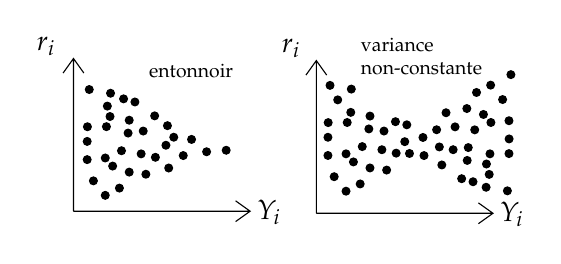
\begin{tikzpicture}[x=0.75pt,y=0.75pt,yscale=-1,xscale=1]
%uncomment if require: \path (0,113.19999694824219); %set diagram left start at 0, and has height of 113.19999694824219

%Shape: Axis 2D [id:dp8558604838271746] 
\draw  (39.32,90.58) -- (124.43,90.58)(39.32,17) -- (39.32,90.58) -- cycle (117.43,85.58) -- (124.43,90.58) -- (117.43,95.58) (34.32,24) -- (39.32,17) -- (44.32,24)  ;
%Flowchart: Connector [id:dp13848232871348576] 
\draw  [fill={rgb, 255:red, 0; green, 0; blue, 0 }  ,fill opacity=1 ] (90.32,63.76) .. controls (90.32,62.72) and (91.16,61.88) .. (92.21,61.88) .. controls (93.25,61.88) and (94.09,62.72) .. (94.09,63.76) .. controls (94.09,64.81) and (93.25,65.65) .. (92.21,65.65) .. controls (91.16,65.65) and (90.32,64.81) .. (90.32,63.76) -- cycle ;
%Flowchart: Connector [id:dp9066276103858408] 
\draw  [fill={rgb, 255:red, 0; green, 0; blue, 0 }  ,fill opacity=1 ] (76.55,44.64) .. controls (76.55,43.6) and (77.4,42.76) .. (78.44,42.76) .. controls (79.48,42.76) and (80.32,43.6) .. (80.32,44.64) .. controls (80.32,45.68) and (79.48,46.53) .. (78.44,46.53) .. controls (77.4,46.53) and (76.55,45.68) .. (76.55,44.64) -- cycle ;
%Flowchart: Connector [id:dp30514499125898076] 
\draw  [fill={rgb, 255:red, 0; green, 0; blue, 0 }  ,fill opacity=1 ] (94.32,55.99) .. controls (94.32,54.95) and (95.16,54.1) .. (96.21,54.1) .. controls (97.25,54.1) and (98.09,54.95) .. (98.09,55.99) .. controls (98.09,57.03) and (97.25,57.88) .. (96.21,57.88) .. controls (95.16,57.88) and (94.32,57.03) .. (94.32,55.99) -- cycle ;
%Flowchart: Connector [id:dp1781117261839127] 
\draw  [fill={rgb, 255:red, 0; green, 0; blue, 0 }  ,fill opacity=1 ] (76.9,64.61) .. controls (76.9,63.56) and (77.75,62.72) .. (78.79,62.72) .. controls (79.83,62.72) and (80.68,63.56) .. (80.68,64.61) .. controls (80.68,65.65) and (79.83,66.49) .. (78.79,66.49) .. controls (77.75,66.49) and (76.9,65.65) .. (76.9,64.61) -- cycle ;
%Flowchart: Connector [id:dp9319859207968288] 
\draw  [fill={rgb, 255:red, 0; green, 0; blue, 0 }  ,fill opacity=1 ] (81.98,58.8) .. controls (81.98,57.76) and (82.83,56.91) .. (83.87,56.91) .. controls (84.91,56.91) and (85.76,57.76) .. (85.76,58.8) .. controls (85.76,59.84) and (84.91,60.69) .. (83.87,60.69) .. controls (82.83,60.69) and (81.98,59.84) .. (81.98,58.8) -- cycle ;
%Flowchart: Connector [id:dp7599303260445949] 
\draw  [fill={rgb, 255:red, 0; green, 0; blue, 0 }  ,fill opacity=1 ] (101.58,61.94) .. controls (101.58,60.9) and (102.42,60.05) .. (103.46,60.05) .. controls (104.5,60.05) and (105.35,60.9) .. (105.35,61.94) .. controls (105.35,62.98) and (104.5,63.83) .. (103.46,63.83) .. controls (102.42,63.83) and (101.58,62.98) .. (101.58,61.94) -- cycle ;
%Flowchart: Connector [id:dp37816906840787734] 
\draw  [fill={rgb, 255:red, 0; green, 0; blue, 0 }  ,fill opacity=1 ] (111.01,61.22) .. controls (111.01,60.17) and (111.85,59.33) .. (112.9,59.33) .. controls (113.94,59.33) and (114.78,60.17) .. (114.78,61.22) .. controls (114.78,62.26) and (113.94,63.1) .. (112.9,63.1) .. controls (111.85,63.1) and (111.01,62.26) .. (111.01,61.22) -- cycle ;
%Flowchart: Connector [id:dp5092304345774592] 
\draw  [fill={rgb, 255:red, 0; green, 0; blue, 0 }  ,fill opacity=1 ] (63.75,52.93) .. controls (63.75,51.89) and (64.59,51.05) .. (65.63,51.05) .. controls (66.67,51.05) and (67.52,51.89) .. (67.52,52.93) .. controls (67.52,53.98) and (66.67,54.82) .. (65.63,54.82) .. controls (64.59,54.82) and (63.75,53.98) .. (63.75,52.93) -- cycle ;
%Flowchart: Connector [id:dp7699746327071277] 
\draw  [fill={rgb, 255:red, 0; green, 0; blue, 0 }  ,fill opacity=1 ] (55.04,44.95) .. controls (55.04,43.91) and (55.88,43.07) .. (56.92,43.07) .. controls (57.97,43.07) and (58.81,43.91) .. (58.81,44.95) .. controls (58.81,45.99) and (57.97,46.84) .. (56.92,46.84) .. controls (55.88,46.84) and (55.04,45.99) .. (55.04,44.95) -- cycle ;
%Flowchart: Connector [id:dp6639592567098165] 
\draw  [fill={rgb, 255:red, 0; green, 0; blue, 0 }  ,fill opacity=1 ] (82.71,49.37) .. controls (82.71,48.33) and (83.55,47.48) .. (84.6,47.48) .. controls (85.64,47.48) and (86.48,48.33) .. (86.48,49.37) .. controls (86.48,50.41) and (85.64,51.25) .. (84.6,51.25) .. controls (83.55,51.25) and (82.71,50.41) .. (82.71,49.37) -- cycle ;
%Flowchart: Connector [id:dp21109171036938168] 
\draw  [fill={rgb, 255:red, 0; green, 0; blue, 0 }  ,fill opacity=1 ] (44.15,49.89) .. controls (44.15,48.84) and (45,48) .. (46.04,48) .. controls (47.08,48) and (47.93,48.84) .. (47.93,49.89) .. controls (47.93,50.93) and (47.08,51.77) .. (46.04,51.77) .. controls (45,51.77) and (44.15,50.93) .. (44.15,49.89) -- cycle ;
%Shape: Axis 2D [id:dp44906440712605544] 
\draw  (156.32,91.58) -- (241.43,91.58)(156.32,18) -- (156.32,91.58) -- cycle (234.43,86.58) -- (241.43,91.58) -- (234.43,96.58) (151.32,25) -- (156.32,18) -- (161.32,25)  ;
%Flowchart: Connector [id:dp510245524022007] 
\draw  [fill={rgb, 255:red, 0; green, 0; blue, 0 }  ,fill opacity=1 ] (85.75,54.93) .. controls (85.75,53.89) and (86.59,53.05) .. (87.63,53.05) .. controls (88.67,53.05) and (89.52,53.89) .. (89.52,54.93) .. controls (89.52,55.98) and (88.67,56.82) .. (87.63,56.82) .. controls (86.59,56.82) and (85.75,55.98) .. (85.75,54.93) -- cycle ;
%Flowchart: Connector [id:dp06596066699721548] 
\draw  [fill={rgb, 255:red, 0; green, 0; blue, 0 }  ,fill opacity=1 ] (71.04,51.95) .. controls (71.04,50.91) and (71.88,50.07) .. (72.92,50.07) .. controls (73.97,50.07) and (74.81,50.91) .. (74.81,51.95) .. controls (74.81,52.99) and (73.97,53.84) .. (72.92,53.84) .. controls (71.88,53.84) and (71.04,52.99) .. (71.04,51.95) -- cycle ;
%Flowchart: Connector [id:dp7786056870830953] 
\draw  [fill={rgb, 255:red, 0; green, 0; blue, 0 }  ,fill opacity=1 ] (59.57,79.45) .. controls (59.57,78.4) and (60.41,77.56) .. (61.46,77.56) .. controls (62.5,77.56) and (63.34,78.4) .. (63.34,79.45) .. controls (63.34,80.49) and (62.5,81.33) .. (61.46,81.33) .. controls (60.41,81.33) and (59.57,80.49) .. (59.57,79.45) -- cycle ;
%Flowchart: Connector [id:dp0017160037187040622] 
\draw  [fill={rgb, 255:red, 0; green, 0; blue, 0 }  ,fill opacity=1 ] (64.29,71.74) .. controls (64.29,70.7) and (65.14,69.85) .. (66.18,69.85) .. controls (67.22,69.85) and (68.07,70.7) .. (68.07,71.74) .. controls (68.07,72.78) and (67.22,73.63) .. (66.18,73.63) .. controls (65.14,73.63) and (64.29,72.78) .. (64.29,71.74) -- cycle ;
%Flowchart: Connector [id:dp5947951522664079] 
\draw  [fill={rgb, 255:red, 0; green, 0; blue, 0 }  ,fill opacity=1 ] (56.31,68.84) .. controls (56.31,67.8) and (57.16,66.95) .. (58.2,66.95) .. controls (59.24,66.95) and (60.09,67.8) .. (60.09,68.84) .. controls (60.09,69.88) and (59.24,70.72) .. (58.2,70.72) .. controls (57.16,70.72) and (56.31,69.88) .. (56.31,68.84) -- cycle ;
%Flowchart: Connector [id:dp06108481790402043] 
\draw  [fill={rgb, 255:red, 0; green, 0; blue, 0 }  ,fill opacity=1 ] (52.75,82.93) .. controls (52.75,81.89) and (53.59,81.05) .. (54.63,81.05) .. controls (55.67,81.05) and (56.52,81.89) .. (56.52,82.93) .. controls (56.52,83.98) and (55.67,84.82) .. (54.63,84.82) .. controls (53.59,84.82) and (52.75,83.98) .. (52.75,82.93) -- cycle ;
%Flowchart: Connector [id:dp15453108419055894] 
\draw  [fill={rgb, 255:red, 0; green, 0; blue, 0 }  ,fill opacity=1 ] (47.04,75.95) .. controls (47.04,74.91) and (47.88,74.07) .. (48.92,74.07) .. controls (49.97,74.07) and (50.81,74.91) .. (50.81,75.95) .. controls (50.81,76.99) and (49.97,77.84) .. (48.92,77.84) .. controls (47.88,77.84) and (47.04,76.99) .. (47.04,75.95) -- cycle ;
%Flowchart: Connector [id:dp5406116279466717] 
\draw  [fill={rgb, 255:red, 0; green, 0; blue, 0 }  ,fill opacity=1 ] (60.57,61.45) .. controls (60.57,60.4) and (61.41,59.56) .. (62.46,59.56) .. controls (63.5,59.56) and (64.34,60.4) .. (64.34,61.45) .. controls (64.34,62.49) and (63.5,63.33) .. (62.46,63.33) .. controls (61.41,63.33) and (60.57,62.49) .. (60.57,61.45) -- cycle ;
%Flowchart: Connector [id:dp5356920731215311] 
\draw  [fill={rgb, 255:red, 0; green, 0; blue, 0 }  ,fill opacity=1 ] (64.29,46.74) .. controls (64.29,45.7) and (65.14,44.85) .. (66.18,44.85) .. controls (67.22,44.85) and (68.07,45.7) .. (68.07,46.74) .. controls (68.07,47.78) and (67.22,48.63) .. (66.18,48.63) .. controls (65.14,48.63) and (64.29,47.78) .. (64.29,46.74) -- cycle ;
%Flowchart: Connector [id:dp759324640569528] 
\draw  [fill={rgb, 255:red, 0; green, 0; blue, 0 }  ,fill opacity=1 ] (53.31,49.84) .. controls (53.31,48.8) and (54.16,47.95) .. (55.2,47.95) .. controls (56.24,47.95) and (57.09,48.8) .. (57.09,49.84) .. controls (57.09,50.88) and (56.24,51.72) .. (55.2,51.72) .. controls (54.16,51.72) and (53.31,50.88) .. (53.31,49.84) -- cycle ;
%Flowchart: Connector [id:dp861574482085449] 
\draw  [fill={rgb, 255:red, 0; green, 0; blue, 0 }  ,fill opacity=1 ] (52.75,64.93) .. controls (52.75,63.89) and (53.59,63.05) .. (54.63,63.05) .. controls (55.67,63.05) and (56.52,63.89) .. (56.52,64.93) .. controls (56.52,65.98) and (55.67,66.82) .. (54.63,66.82) .. controls (53.59,66.82) and (52.75,65.98) .. (52.75,64.93) -- cycle ;
%Flowchart: Connector [id:dp3067212479481558] 
\draw  [fill={rgb, 255:red, 0; green, 0; blue, 0 }  ,fill opacity=1 ] (44.04,56.95) .. controls (44.04,55.91) and (44.88,55.07) .. (45.92,55.07) .. controls (46.97,55.07) and (47.81,55.91) .. (47.81,56.95) .. controls (47.81,57.99) and (46.97,58.84) .. (45.92,58.84) .. controls (44.88,58.84) and (44.04,57.99) .. (44.04,56.95) -- cycle ;
%Flowchart: Connector [id:dp4250502580638582] 
\draw  [fill={rgb, 255:red, 0; green, 0; blue, 0 }  ,fill opacity=1 ] (70.04,62.95) .. controls (70.04,61.91) and (70.88,61.07) .. (71.92,61.07) .. controls (72.97,61.07) and (73.81,61.91) .. (73.81,62.95) .. controls (73.81,63.99) and (72.97,64.84) .. (71.92,64.84) .. controls (70.88,64.84) and (70.04,63.99) .. (70.04,62.95) -- cycle ;
%Flowchart: Connector [id:dp21805877508339333] 
\draw  [fill={rgb, 255:red, 0; green, 0; blue, 0 }  ,fill opacity=1 ] (61.57,36.45) .. controls (61.57,35.4) and (62.41,34.56) .. (63.46,34.56) .. controls (64.5,34.56) and (65.34,35.4) .. (65.34,36.45) .. controls (65.34,37.49) and (64.5,38.33) .. (63.46,38.33) .. controls (62.41,38.33) and (61.57,37.49) .. (61.57,36.45) -- cycle ;
%Flowchart: Connector [id:dp13755122925998542] 
\draw  [fill={rgb, 255:red, 0; green, 0; blue, 0 }  ,fill opacity=1 ] (55.29,33.74) .. controls (55.29,32.7) and (56.14,31.85) .. (57.18,31.85) .. controls (58.22,31.85) and (59.07,32.7) .. (59.07,33.74) .. controls (59.07,34.78) and (58.22,35.63) .. (57.18,35.63) .. controls (56.14,35.63) and (55.29,34.78) .. (55.29,33.74) -- cycle ;
%Flowchart: Connector [id:dp9720404055907759] 
\draw  [fill={rgb, 255:red, 0; green, 0; blue, 0 }  ,fill opacity=1 ] (44.04,65.73) .. controls (44.04,64.68) and (44.88,63.84) .. (45.92,63.84) .. controls (46.97,63.84) and (47.81,64.68) .. (47.81,65.73) .. controls (47.81,66.77) and (46.97,67.61) .. (45.92,67.61) .. controls (44.88,67.61) and (44.04,66.77) .. (44.04,65.73) -- cycle ;
%Flowchart: Connector [id:dp6879320647514107] 
\draw  [fill={rgb, 255:red, 0; green, 0; blue, 0 }  ,fill opacity=1 ] (53.75,39.93) .. controls (53.75,38.89) and (54.59,38.05) .. (55.63,38.05) .. controls (56.67,38.05) and (57.52,38.89) .. (57.52,39.93) .. controls (57.52,40.98) and (56.67,41.82) .. (55.63,41.82) .. controls (54.59,41.82) and (53.75,40.98) .. (53.75,39.93) -- cycle ;
%Flowchart: Connector [id:dp04951146450025434] 
\draw  [fill={rgb, 255:red, 0; green, 0; blue, 0 }  ,fill opacity=1 ] (45.04,31.95) .. controls (45.04,30.91) and (45.88,30.07) .. (46.92,30.07) .. controls (47.97,30.07) and (48.81,30.91) .. (48.81,31.95) .. controls (48.81,32.99) and (47.97,33.84) .. (46.92,33.84) .. controls (45.88,33.84) and (45.04,32.99) .. (45.04,31.95) -- cycle ;
%Flowchart: Connector [id:dp41316709921664807] 
\draw  [fill={rgb, 255:red, 0; green, 0; blue, 0 }  ,fill opacity=1 ] (67.04,37.95) .. controls (67.04,36.91) and (67.88,36.07) .. (68.92,36.07) .. controls (69.97,36.07) and (70.81,36.91) .. (70.81,37.95) .. controls (70.81,38.99) and (69.97,39.84) .. (68.92,39.84) .. controls (67.88,39.84) and (67.04,38.99) .. (67.04,37.95) -- cycle ;
%Flowchart: Connector [id:dp7236329878048122] 
\draw  [fill={rgb, 255:red, 0; green, 0; blue, 0 }  ,fill opacity=1 ] (83.32,69.76) .. controls (83.32,68.72) and (84.16,67.88) .. (85.21,67.88) .. controls (86.25,67.88) and (87.09,68.72) .. (87.09,69.76) .. controls (87.09,70.81) and (86.25,71.65) .. (85.21,71.65) .. controls (84.16,71.65) and (83.32,70.81) .. (83.32,69.76) -- cycle ;
%Flowchart: Connector [id:dp42964405575689435] 
\draw  [fill={rgb, 255:red, 0; green, 0; blue, 0 }  ,fill opacity=1 ] (72.32,72.76) .. controls (72.32,71.72) and (73.16,70.88) .. (74.21,70.88) .. controls (75.25,70.88) and (76.09,71.72) .. (76.09,72.76) .. controls (76.09,73.81) and (75.25,74.65) .. (74.21,74.65) .. controls (73.16,74.65) and (72.32,73.81) .. (72.32,72.76) -- cycle ;
%Flowchart: Connector [id:dp6747024208184615] 
\draw  [fill={rgb, 255:red, 0; green, 0; blue, 0 }  ,fill opacity=1 ] (206.32,63.76) .. controls (206.32,62.72) and (207.16,61.88) .. (208.21,61.88) .. controls (209.25,61.88) and (210.09,62.72) .. (210.09,63.76) .. controls (210.09,64.81) and (209.25,65.65) .. (208.21,65.65) .. controls (207.16,65.65) and (206.32,64.81) .. (206.32,63.76) -- cycle ;
%Flowchart: Connector [id:dp375207162457027] 
\draw  [fill={rgb, 255:red, 0; green, 0; blue, 0 }  ,fill opacity=1 ] (192.9,62.61) .. controls (192.9,61.56) and (193.75,60.72) .. (194.79,60.72) .. controls (195.83,60.72) and (196.68,61.56) .. (196.68,62.61) .. controls (196.68,63.65) and (195.83,64.49) .. (194.79,64.49) .. controls (193.75,64.49) and (192.9,63.65) .. (192.9,62.61) -- cycle ;
%Flowchart: Connector [id:dp3530540543397802] 
\draw  [fill={rgb, 255:red, 0; green, 0; blue, 0 }  ,fill opacity=1 ] (179.75,50.93) .. controls (179.75,49.89) and (180.59,49.05) .. (181.63,49.05) .. controls (182.67,49.05) and (183.52,49.89) .. (183.52,50.93) .. controls (183.52,51.98) and (182.67,52.82) .. (181.63,52.82) .. controls (180.59,52.82) and (179.75,51.98) .. (179.75,50.93) -- cycle ;
%Flowchart: Connector [id:dp9278174177870371] 
\draw  [fill={rgb, 255:red, 0; green, 0; blue, 0 }  ,fill opacity=1 ] (171.04,42.95) .. controls (171.04,41.91) and (171.88,41.07) .. (172.92,41.07) .. controls (173.97,41.07) and (174.81,41.91) .. (174.81,42.95) .. controls (174.81,43.99) and (173.97,44.84) .. (172.92,44.84) .. controls (171.88,44.84) and (171.04,43.99) .. (171.04,42.95) -- cycle ;
%Flowchart: Connector [id:dp7721407861275282] 
\draw  [fill={rgb, 255:red, 0; green, 0; blue, 0 }  ,fill opacity=1 ] (160.15,47.89) .. controls (160.15,46.84) and (161,46) .. (162.04,46) .. controls (163.08,46) and (163.93,46.84) .. (163.93,47.89) .. controls (163.93,48.93) and (163.08,49.77) .. (162.04,49.77) .. controls (161,49.77) and (160.15,48.93) .. (160.15,47.89) -- cycle ;
%Flowchart: Connector [id:dp4079068221945319] 
\draw  [fill={rgb, 255:red, 0; green, 0; blue, 0 }  ,fill opacity=1 ] (187.04,51.95) .. controls (187.04,50.91) and (187.88,50.07) .. (188.92,50.07) .. controls (189.97,50.07) and (190.81,50.91) .. (190.81,51.95) .. controls (190.81,52.99) and (189.97,53.84) .. (188.92,53.84) .. controls (187.88,53.84) and (187.04,52.99) .. (187.04,51.95) -- cycle ;
%Flowchart: Connector [id:dp5475908699877261] 
\draw  [fill={rgb, 255:red, 0; green, 0; blue, 0 }  ,fill opacity=1 ] (175.57,77.45) .. controls (175.57,76.4) and (176.41,75.56) .. (177.46,75.56) .. controls (178.5,75.56) and (179.34,76.4) .. (179.34,77.45) .. controls (179.34,78.49) and (178.5,79.33) .. (177.46,79.33) .. controls (176.41,79.33) and (175.57,78.49) .. (175.57,77.45) -- cycle ;
%Flowchart: Connector [id:dp04436194109667668] 
\draw  [fill={rgb, 255:red, 0; green, 0; blue, 0 }  ,fill opacity=1 ] (180.29,69.74) .. controls (180.29,68.7) and (181.14,67.85) .. (182.18,67.85) .. controls (183.22,67.85) and (184.07,68.7) .. (184.07,69.74) .. controls (184.07,70.78) and (183.22,71.63) .. (182.18,71.63) .. controls (181.14,71.63) and (180.29,70.78) .. (180.29,69.74) -- cycle ;
%Flowchart: Connector [id:dp16435595480811171] 
\draw  [fill={rgb, 255:red, 0; green, 0; blue, 0 }  ,fill opacity=1 ] (172.31,66.84) .. controls (172.31,65.8) and (173.16,64.95) .. (174.2,64.95) .. controls (175.24,64.95) and (176.09,65.8) .. (176.09,66.84) .. controls (176.09,67.88) and (175.24,68.72) .. (174.2,68.72) .. controls (173.16,68.72) and (172.31,67.88) .. (172.31,66.84) -- cycle ;
%Flowchart: Connector [id:dp8368581493636196] 
\draw  [fill={rgb, 255:red, 0; green, 0; blue, 0 }  ,fill opacity=1 ] (168.75,80.93) .. controls (168.75,79.89) and (169.59,79.05) .. (170.63,79.05) .. controls (171.67,79.05) and (172.52,79.89) .. (172.52,80.93) .. controls (172.52,81.98) and (171.67,82.82) .. (170.63,82.82) .. controls (169.59,82.82) and (168.75,81.98) .. (168.75,80.93) -- cycle ;
%Flowchart: Connector [id:dp46353263152743907] 
\draw  [fill={rgb, 255:red, 0; green, 0; blue, 0 }  ,fill opacity=1 ] (163.04,73.95) .. controls (163.04,72.91) and (163.88,72.07) .. (164.92,72.07) .. controls (165.97,72.07) and (166.81,72.91) .. (166.81,73.95) .. controls (166.81,74.99) and (165.97,75.84) .. (164.92,75.84) .. controls (163.88,75.84) and (163.04,74.99) .. (163.04,73.95) -- cycle ;
%Flowchart: Connector [id:dp3001260665534562] 
\draw  [fill={rgb, 255:red, 0; green, 0; blue, 0 }  ,fill opacity=1 ] (176.57,59.45) .. controls (176.57,58.4) and (177.41,57.56) .. (178.46,57.56) .. controls (179.5,57.56) and (180.34,58.4) .. (180.34,59.45) .. controls (180.34,60.49) and (179.5,61.33) .. (178.46,61.33) .. controls (177.41,61.33) and (176.57,60.49) .. (176.57,59.45) -- cycle ;
%Flowchart: Connector [id:dp41866699667800766] 
\draw  [fill={rgb, 255:red, 0; green, 0; blue, 0 }  ,fill opacity=1 ] (180.29,44.74) .. controls (180.29,43.7) and (181.14,42.85) .. (182.18,42.85) .. controls (183.22,42.85) and (184.07,43.7) .. (184.07,44.74) .. controls (184.07,45.78) and (183.22,46.63) .. (182.18,46.63) .. controls (181.14,46.63) and (180.29,45.78) .. (180.29,44.74) -- cycle ;
%Flowchart: Connector [id:dp7824227734018141] 
\draw  [fill={rgb, 255:red, 0; green, 0; blue, 0 }  ,fill opacity=1 ] (169.31,47.84) .. controls (169.31,46.8) and (170.16,45.95) .. (171.2,45.95) .. controls (172.24,45.95) and (173.09,46.8) .. (173.09,47.84) .. controls (173.09,48.88) and (172.24,49.72) .. (171.2,49.72) .. controls (170.16,49.72) and (169.31,48.88) .. (169.31,47.84) -- cycle ;
%Flowchart: Connector [id:dp555845877698876] 
\draw  [fill={rgb, 255:red, 0; green, 0; blue, 0 }  ,fill opacity=1 ] (168.75,62.93) .. controls (168.75,61.89) and (169.59,61.05) .. (170.63,61.05) .. controls (171.67,61.05) and (172.52,61.89) .. (172.52,62.93) .. controls (172.52,63.98) and (171.67,64.82) .. (170.63,64.82) .. controls (169.59,64.82) and (168.75,63.98) .. (168.75,62.93) -- cycle ;
%Flowchart: Connector [id:dp9006024154568015] 
\draw  [fill={rgb, 255:red, 0; green, 0; blue, 0 }  ,fill opacity=1 ] (160.04,54.95) .. controls (160.04,53.91) and (160.88,53.07) .. (161.92,53.07) .. controls (162.97,53.07) and (163.81,53.91) .. (163.81,54.95) .. controls (163.81,55.99) and (162.97,56.84) .. (161.92,56.84) .. controls (160.88,56.84) and (160.04,55.99) .. (160.04,54.95) -- cycle ;
%Flowchart: Connector [id:dp26233305592629863] 
\draw  [fill={rgb, 255:red, 0; green, 0; blue, 0 }  ,fill opacity=1 ] (186.04,60.95) .. controls (186.04,59.91) and (186.88,59.07) .. (187.92,59.07) .. controls (188.97,59.07) and (189.81,59.91) .. (189.81,60.95) .. controls (189.81,61.99) and (188.97,62.84) .. (187.92,62.84) .. controls (186.88,62.84) and (186.04,61.99) .. (186.04,60.95) -- cycle ;
%Flowchart: Connector [id:dp5500604107313869] 
\draw  [fill={rgb, 255:red, 0; green, 0; blue, 0 }  ,fill opacity=1 ] (192.57,47.45) .. controls (192.57,46.4) and (193.41,45.56) .. (194.46,45.56) .. controls (195.5,45.56) and (196.34,46.4) .. (196.34,47.45) .. controls (196.34,48.49) and (195.5,49.33) .. (194.46,49.33) .. controls (193.41,49.33) and (192.57,48.49) .. (192.57,47.45) -- cycle ;
%Flowchart: Connector [id:dp007297969493494705] 
\draw  [fill={rgb, 255:red, 0; green, 0; blue, 0 }  ,fill opacity=1 ] (171.29,31.74) .. controls (171.29,30.7) and (172.14,29.85) .. (173.18,29.85) .. controls (174.22,29.85) and (175.07,30.7) .. (175.07,31.74) .. controls (175.07,32.78) and (174.22,33.63) .. (173.18,33.63) .. controls (172.14,33.63) and (171.29,32.78) .. (171.29,31.74) -- cycle ;
%Flowchart: Connector [id:dp5240179352272871] 
\draw  [fill={rgb, 255:red, 0; green, 0; blue, 0 }  ,fill opacity=1 ] (160.04,63.73) .. controls (160.04,62.68) and (160.88,61.84) .. (161.92,61.84) .. controls (162.97,61.84) and (163.81,62.68) .. (163.81,63.73) .. controls (163.81,64.77) and (162.97,65.61) .. (161.92,65.61) .. controls (160.88,65.61) and (160.04,64.77) .. (160.04,63.73) -- cycle ;
%Flowchart: Connector [id:dp4529602471979908] 
\draw  [fill={rgb, 255:red, 0; green, 0; blue, 0 }  ,fill opacity=1 ] (164.75,36.93) .. controls (164.75,35.89) and (165.59,35.05) .. (166.63,35.05) .. controls (167.67,35.05) and (168.52,35.89) .. (168.52,36.93) .. controls (168.52,37.98) and (167.67,38.82) .. (166.63,38.82) .. controls (165.59,38.82) and (164.75,37.98) .. (164.75,36.93) -- cycle ;
%Flowchart: Connector [id:dp3595134810790366] 
\draw  [fill={rgb, 255:red, 0; green, 0; blue, 0 }  ,fill opacity=1 ] (161.04,29.95) .. controls (161.04,28.91) and (161.88,28.07) .. (162.92,28.07) .. controls (163.97,28.07) and (164.81,28.91) .. (164.81,29.95) .. controls (164.81,30.99) and (163.97,31.84) .. (162.92,31.84) .. controls (161.88,31.84) and (161.04,30.99) .. (161.04,29.95) -- cycle ;
%Flowchart: Connector [id:dp08959844386091564] 
\draw  [fill={rgb, 255:red, 0; green, 0; blue, 0 }  ,fill opacity=1 ] (198.04,48.95) .. controls (198.04,47.91) and (198.88,47.07) .. (199.92,47.07) .. controls (200.97,47.07) and (201.81,47.91) .. (201.81,48.95) .. controls (201.81,49.99) and (200.97,50.84) .. (199.92,50.84) .. controls (198.88,50.84) and (198.04,49.99) .. (198.04,48.95) -- cycle ;
%Flowchart: Connector [id:dp9483524226268623] 
\draw  [fill={rgb, 255:red, 0; green, 0; blue, 0 }  ,fill opacity=1 ] (199.32,62.76) .. controls (199.32,61.72) and (200.16,60.88) .. (201.21,60.88) .. controls (202.25,60.88) and (203.09,61.72) .. (203.09,62.76) .. controls (203.09,63.81) and (202.25,64.65) .. (201.21,64.65) .. controls (200.16,64.65) and (199.32,63.81) .. (199.32,62.76) -- cycle ;
%Flowchart: Connector [id:dp708522000017336] 
\draw  [fill={rgb, 255:red, 0; green, 0; blue, 0 }  ,fill opacity=1 ] (188.32,70.76) .. controls (188.32,69.72) and (189.16,68.88) .. (190.21,68.88) .. controls (191.25,68.88) and (192.09,69.72) .. (192.09,70.76) .. controls (192.09,71.81) and (191.25,72.65) .. (190.21,72.65) .. controls (189.16,72.65) and (188.32,71.81) .. (188.32,70.76) -- cycle ;
%Flowchart: Connector [id:dp12449484934713428] 
\draw  [fill={rgb, 255:red, 0; green, 0; blue, 0 }  ,fill opacity=1 ] (218.67,68.28) .. controls (218.68,69.33) and (217.84,70.18) .. (216.8,70.18) .. controls (215.76,70.19) and (214.91,69.35) .. (214.9,68.31) .. controls (214.89,67.27) and (215.73,66.42) .. (216.77,66.41) .. controls (217.81,66.4) and (218.66,67.24) .. (218.67,68.28) -- cycle ;
%Flowchart: Connector [id:dp3873681254454473] 
\draw  [fill={rgb, 255:red, 0; green, 0; blue, 0 }  ,fill opacity=1 ] (200.82,57.06) .. controls (200.83,58.1) and (199.99,58.96) .. (198.95,58.96) .. controls (197.91,58.97) and (197.06,58.13) .. (197.05,57.09) .. controls (197.04,56.05) and (197.88,55.2) .. (198.92,55.19) .. controls (199.96,55.18) and (200.82,56.02) .. (200.82,57.06) -- cycle ;
%Flowchart: Connector [id:dp9779431254977391] 
\draw  [fill={rgb, 255:red, 0; green, 0; blue, 0 }  ,fill opacity=1 ] (216.18,51.32) .. controls (216.18,52.37) and (215.34,53.22) .. (214.3,53.22) .. controls (213.26,53.23) and (212.41,52.39) .. (212.4,51.35) .. controls (212.39,50.31) and (213.23,49.46) .. (214.28,49.45) .. controls (215.32,49.44) and (216.17,50.28) .. (216.18,51.32) -- cycle ;
%Flowchart: Connector [id:dp9406191265438184] 
\draw  [fill={rgb, 255:red, 0; green, 0; blue, 0 }  ,fill opacity=1 ] (231.42,59.9) .. controls (231.42,60.94) and (230.59,61.79) .. (229.54,61.8) .. controls (228.5,61.81) and (227.65,60.97) .. (227.64,59.93) .. controls (227.64,58.89) and (228.48,58.03) .. (229.52,58.03) .. controls (230.56,58.02) and (231.41,58.86) .. (231.42,59.9) -- cycle ;
%Flowchart: Connector [id:dp43445741827300144] 
\draw  [fill={rgb, 255:red, 0; green, 0; blue, 0 }  ,fill opacity=1 ] (240.18,67.82) .. controls (240.19,68.86) and (239.35,69.71) .. (238.31,69.72) .. controls (237.27,69.73) and (236.42,68.89) .. (236.41,67.85) .. controls (236.4,66.8) and (237.24,65.95) .. (238.28,65.95) .. controls (239.32,65.94) and (240.17,66.78) .. (240.18,67.82) -- cycle ;
%Flowchart: Connector [id:dp5286611433310382] 
\draw  [fill={rgb, 255:red, 0; green, 0; blue, 0 }  ,fill opacity=1 ] (217.48,59.6) .. controls (217.49,60.64) and (216.65,61.5) .. (215.61,61.5) .. controls (214.56,61.51) and (213.71,60.67) .. (213.71,59.63) .. controls (213.7,58.59) and (214.54,57.74) .. (215.58,57.73) .. controls (216.62,57.72) and (217.47,58.56) .. (217.48,59.6) -- cycle ;
%Flowchart: Connector [id:dp7585404115981156] 
\draw  [fill={rgb, 255:red, 0; green, 0; blue, 0 }  ,fill opacity=1 ] (251.03,62.81) .. controls (251.04,63.85) and (250.2,64.7) .. (249.16,64.71) .. controls (248.12,64.72) and (247.26,63.88) .. (247.26,62.83) .. controls (247.25,61.79) and (248.09,60.94) .. (249.13,60.93) .. controls (250.17,60.93) and (251.02,61.77) .. (251.03,62.81) -- cycle ;
%Flowchart: Connector [id:dp6938348956881057] 
\draw  [fill={rgb, 255:red, 0; green, 0; blue, 0 }  ,fill opacity=1 ] (209.6,55.04) .. controls (209.6,56.08) and (208.76,56.93) .. (207.72,56.94) .. controls (206.68,56.94) and (205.83,56.1) .. (205.82,55.06) .. controls (205.82,54.02) and (206.65,53.17) .. (207.7,53.16) .. controls (208.74,53.16) and (209.59,53.99) .. (209.6,55.04) -- cycle ;
%Flowchart: Connector [id:dp6493600409245479] 
\draw  [fill={rgb, 255:red, 0; green, 0; blue, 0 }  ,fill opacity=1 ] (224.13,60.93) .. controls (224.14,61.98) and (223.3,62.83) .. (222.26,62.83) .. controls (221.22,62.84) and (220.37,62) .. (220.36,60.96) .. controls (220.35,59.92) and (221.19,59.07) .. (222.23,59.06) .. controls (223.27,59.05) and (224.12,59.89) .. (224.13,60.93) -- cycle ;
%Flowchart: Connector [id:dp7480096411288237] 
\draw  [fill={rgb, 255:red, 0; green, 0; blue, 0 }  ,fill opacity=1 ] (235.4,33.36) .. controls (235.41,34.4) and (234.57,35.25) .. (233.53,35.26) .. controls (232.49,35.27) and (231.64,34.43) .. (231.63,33.39) .. controls (231.62,32.34) and (232.46,31.49) .. (233.5,31.49) .. controls (234.55,31.48) and (235.4,32.32) .. (235.4,33.36) -- cycle ;
%Flowchart: Connector [id:dp88287472504798] 
\draw  [fill={rgb, 255:red, 0; green, 0; blue, 0 }  ,fill opacity=1 ] (230.73,41.1) .. controls (230.74,42.14) and (229.9,42.99) .. (228.86,43) .. controls (227.82,43.01) and (226.97,42.17) .. (226.96,41.13) .. controls (226.95,40.08) and (227.79,39.23) .. (228.83,39.23) .. controls (229.88,39.22) and (230.73,40.06) .. (230.73,41.1) -- cycle ;
%Flowchart: Connector [id:dp6651691157334751] 
\draw  [fill={rgb, 255:red, 0; green, 0; blue, 0 }  ,fill opacity=1 ] (238.74,43.94) .. controls (238.74,44.99) and (237.91,45.84) .. (236.86,45.85) .. controls (235.82,45.85) and (234.97,45.01) .. (234.96,43.97) .. controls (234.96,42.93) and (235.79,42.08) .. (236.84,42.07) .. controls (237.88,42.06) and (238.73,42.9) .. (238.74,43.94) -- cycle ;
%Flowchart: Connector [id:dp7496637067038703] 
\draw  [fill={rgb, 255:red, 0; green, 0; blue, 0 }  ,fill opacity=1 ] (242.2,29.82) .. controls (242.21,30.86) and (241.37,31.71) .. (240.33,31.72) .. controls (239.29,31.73) and (238.44,30.89) .. (238.43,29.85) .. controls (238.42,28.81) and (239.26,27.96) .. (240.3,27.95) .. controls (241.34,27.94) and (242.19,28.78) .. (242.2,29.82) -- cycle ;
%Flowchart: Connector [id:dp8854415375047968] 
\draw  [fill={rgb, 255:red, 0; green, 0; blue, 0 }  ,fill opacity=1 ] (247.96,36.76) .. controls (247.97,37.81) and (247.13,38.66) .. (246.09,38.66) .. controls (245.04,38.67) and (244.19,37.83) .. (244.19,36.79) .. controls (244.18,35.75) and (245.02,34.9) .. (246.06,34.89) .. controls (247.1,34.88) and (247.95,35.72) .. (247.96,36.76) -- cycle ;
%Flowchart: Connector [id:dp7412916275222396] 
\draw  [fill={rgb, 255:red, 0; green, 0; blue, 0 }  ,fill opacity=1 ] (234.53,51.37) .. controls (234.54,52.41) and (233.7,53.26) .. (232.66,53.27) .. controls (231.62,53.27) and (230.77,52.43) .. (230.76,51.39) .. controls (230.75,50.35) and (231.59,49.5) .. (232.63,49.49) .. controls (233.67,49.48) and (234.53,50.32) .. (234.53,51.37) -- cycle ;
%Flowchart: Connector [id:dp6394005998862176] 
\draw  [fill={rgb, 255:red, 0; green, 0; blue, 0 }  ,fill opacity=1 ] (230.91,66.1) .. controls (230.92,67.14) and (230.08,67.99) .. (229.04,68) .. controls (228,68.01) and (227.15,67.17) .. (227.14,66.13) .. controls (227.13,65.08) and (227.97,64.23) .. (229.01,64.23) .. controls (230.05,64.22) and (230.91,65.06) .. (230.91,66.1) -- cycle ;
%Flowchart: Connector [id:dp735359386617378] 
\draw  [fill={rgb, 255:red, 0; green, 0; blue, 0 }  ,fill opacity=1 ] (241.87,62.92) .. controls (241.88,63.96) and (241.04,64.82) .. (240,64.82) .. controls (238.96,64.83) and (238.11,63.99) .. (238.1,62.95) .. controls (238.09,61.91) and (238.93,61.06) .. (239.97,61.05) .. controls (241.01,61.04) and (241.86,61.88) .. (241.87,62.92) -- cycle ;
%Flowchart: Connector [id:dp13655355437800476] 
\draw  [fill={rgb, 255:red, 0; green, 0; blue, 0 }  ,fill opacity=1 ] (242.33,47.82) .. controls (242.34,48.86) and (241.5,49.71) .. (240.46,49.72) .. controls (239.42,49.73) and (238.57,48.89) .. (238.56,47.85) .. controls (238.55,46.81) and (239.39,45.96) .. (240.43,45.95) .. controls (241.47,45.94) and (242.32,46.78) .. (242.33,47.82) -- cycle ;
%Flowchart: Connector [id:dp3345257989542174] 
\draw  [fill={rgb, 255:red, 0; green, 0; blue, 0 }  ,fill opacity=1 ] (251.1,55.74) .. controls (251.1,56.78) and (250.26,57.63) .. (249.22,57.64) .. controls (248.18,57.65) and (247.33,56.81) .. (247.32,55.77) .. controls (247.31,54.73) and (248.15,53.88) .. (249.2,53.87) .. controls (250.24,53.86) and (251.09,54.7) .. (251.1,55.74) -- cycle ;
%Flowchart: Connector [id:dp8646686868969553] 
\draw  [fill={rgb, 255:red, 0; green, 0; blue, 0 }  ,fill opacity=1 ] (225.05,49.93) .. controls (225.06,50.97) and (224.22,51.82) .. (223.18,51.83) .. controls (222.14,51.83) and (221.29,51) .. (221.28,49.95) .. controls (221.27,48.91) and (222.11,48.06) .. (223.15,48.05) .. controls (224.19,48.05) and (225.05,48.89) .. (225.05,49.93) -- cycle ;
%Flowchart: Connector [id:dp33660457973454916] 
\draw  [fill={rgb, 255:red, 0; green, 0; blue, 0 }  ,fill opacity=1 ] (233.71,76.37) .. controls (233.72,77.41) and (232.88,78.26) .. (231.84,78.27) .. controls (230.8,78.28) and (229.95,77.44) .. (229.94,76.4) .. controls (229.93,75.36) and (230.77,74.51) .. (231.81,74.5) .. controls (232.85,74.49) and (233.7,75.33) .. (233.71,76.37) -- cycle ;
%Flowchart: Connector [id:dp8627832344177755] 
\draw  [fill={rgb, 255:red, 0; green, 0; blue, 0 }  ,fill opacity=1 ] (240.01,79.03) .. controls (240.01,80.08) and (239.17,80.93) .. (238.13,80.93) .. controls (237.09,80.94) and (236.24,80.1) .. (236.23,79.06) .. controls (236.23,78.02) and (237.06,77.17) .. (238.11,77.16) .. controls (239.15,77.15) and (240,77.99) .. (240.01,79.03) -- cycle ;
%Flowchart: Connector [id:dp9501679510769538] 
\draw  [fill={rgb, 255:red, 0; green, 0; blue, 0 }  ,fill opacity=1 ] (251.03,46.97) .. controls (251.04,48.01) and (250.2,48.86) .. (249.16,48.87) .. controls (248.12,48.88) and (247.27,48.04) .. (247.26,47) .. controls (247.25,45.95) and (248.09,45.1) .. (249.13,45.1) .. controls (250.17,45.09) and (251.03,45.93) .. (251.03,46.97) -- cycle ;
%Flowchart: Connector [id:dp11057689212563515] 
\draw  [fill={rgb, 255:red, 0; green, 0; blue, 0 }  ,fill opacity=1 ] (241.51,72.83) .. controls (241.52,73.87) and (240.68,74.72) .. (239.64,74.73) .. controls (238.59,74.74) and (237.74,73.9) .. (237.74,72.86) .. controls (237.73,71.81) and (238.57,70.96) .. (239.61,70.96) .. controls (240.65,70.95) and (241.5,71.79) .. (241.51,72.83) -- cycle ;
%Flowchart: Connector [id:dp8845398486622797] 
\draw  [fill={rgb, 255:red, 0; green, 0; blue, 0 }  ,fill opacity=1 ] (250.27,80.75) .. controls (250.28,81.79) and (249.44,82.64) .. (248.4,82.65) .. controls (247.36,82.66) and (246.51,81.82) .. (246.5,80.77) .. controls (246.49,79.73) and (247.33,78.88) .. (248.37,78.87) .. controls (249.42,78.87) and (250.27,79.71) .. (250.27,80.75) -- cycle ;
%Flowchart: Connector [id:dp1928362619987123] 
\draw  [fill={rgb, 255:red, 0; green, 0; blue, 0 }  ,fill opacity=1 ] (228.23,74.91) .. controls (228.24,75.95) and (227.4,76.8) .. (226.36,76.81) .. controls (225.32,76.81) and (224.47,75.97) .. (224.46,74.93) .. controls (224.45,73.89) and (225.29,73.04) .. (226.33,73.03) .. controls (227.37,73.02) and (228.22,73.86) .. (228.23,74.91) -- cycle ;
%Flowchart: Connector [id:dp5639627141424779] 
\draw  [fill={rgb, 255:red, 0; green, 0; blue, 0 }  ,fill opacity=1 ] (220.7,43.13) .. controls (220.71,44.17) and (219.87,45.02) .. (218.83,45.03) .. controls (217.79,45.04) and (216.94,44.2) .. (216.93,43.16) .. controls (216.92,42.12) and (217.76,41.27) .. (218.8,41.26) .. controls (219.84,41.25) and (220.69,42.09) .. (220.7,43.13) -- cycle ;
%Flowchart: Connector [id:dp7532230419821151] 
\draw  [fill={rgb, 255:red, 0; green, 0; blue, 0 }  ,fill opacity=1 ] (251.96,24.76) .. controls (251.97,25.81) and (251.13,26.66) .. (250.09,26.66) .. controls (249.04,26.67) and (248.19,25.83) .. (248.19,24.79) .. controls (248.18,23.75) and (249.02,22.9) .. (250.06,22.89) .. controls (251.1,22.88) and (251.95,23.72) .. (251.96,24.76) -- cycle ;

% Text Node
\draw (26.26,11.18) node  [align=left] {$\displaystyle r_{i}$};
% Text Node
\draw (133.65,91.02) node  [align=left] {$\displaystyle Y_{i}$};
% Text Node
\draw (250.65,92.02) node  [align=left] {$\displaystyle Y_{i}$};
% Text Node
\draw (144.26,12.18) node  [align=left] {$\displaystyle r_{i}$};
% Text Node
\draw (96,23.2) node [scale=0.7] [align=left] {entonnoir};
% Text Node
\draw (207,16.2) node [scale=0.7] [align=left] {variance \\non-constante};
\end{tikzpicture}

\end{itemize}

\subsubsection*{Indépendance}
Puisque c'est difficile à tester, on peut faire la graphique des résidus en fonction du numéro d'observation pour des données chronologiques.
\begin{itemize}
\item Graphique $r_i|i$ : Si il y a un \textit{pattern}, présence d'auto-corrélation (le postulat $H_3$ n'est donc pas respecté).

\tikzset{every picture/.style={line width=0.75pt}} %set default line width to 0.75pt        

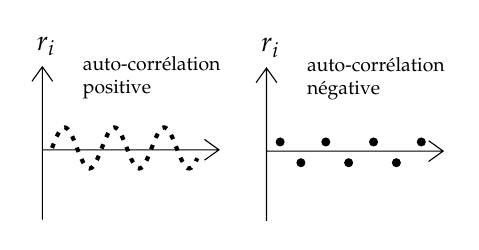
\begin{tikzpicture}[x=0.75pt,y=0.75pt,yscale=-1,xscale=1]
%uncomment if require: \path (0,113.19999694824219); %set diagram left start at 0, and has height of 113.19999694824219

%Shape: Axis 2D [id:dp6079484334131691] 
\draw  (24.32,61) -- (109.43,61)(24.32,21) -- (24.32,94.58) (102.43,56) -- (109.43,61) -- (102.43,66) (19.32,28) -- (24.32,21) -- (29.32,28)  ;
%Shape: Wave [id:dp8253529365925547] 
\draw  [dash pattern={on 1.69pt off 2.76pt}][line width=1.5]  (29,60.1) .. controls (30.96,55.03) and (32.83,50.2) .. (35,50.2) .. controls (37.17,50.2) and (39.04,55.03) .. (41,60.1) .. controls (42.96,65.17) and (44.83,70) .. (47,70) .. controls (49.17,70) and (51.04,65.17) .. (53,60.1) .. controls (54.96,55.03) and (56.83,50.2) .. (59,50.2) .. controls (61.17,50.2) and (63.04,55.03) .. (65,60.1) .. controls (66.96,65.17) and (68.83,70) .. (71,70) .. controls (73.17,70) and (75.04,65.17) .. (77,60.1) .. controls (78.96,55.03) and (80.83,50.2) .. (83,50.2) .. controls (85.17,50.2) and (87.04,55.03) .. (89,60.1) .. controls (90.96,65.17) and (92.83,70) .. (95,70) .. controls (96.43,70) and (97.72,67.92) .. (99,65.05) ;
%Shape: Axis 2D [id:dp23035706266566236] 
\draw  (132.32,61.62) -- (217.43,61.62)(132.32,21.62) -- (132.32,95.2) (210.43,56.62) -- (217.43,61.62) -- (210.43,66.62) (127.32,28.62) -- (132.32,21.62) -- (137.32,28.62)  ;
%Flowchart: Connector [id:dp5178889545560774] 
\draw  [fill={rgb, 255:red, 0; green, 0; blue, 0 }  ,fill opacity=1 ] (137.01,57.22) .. controls (137.01,56.17) and (137.85,55.33) .. (138.9,55.33) .. controls (139.94,55.33) and (140.78,56.17) .. (140.78,57.22) .. controls (140.78,58.26) and (139.94,59.1) .. (138.9,59.1) .. controls (137.85,59.1) and (137.01,58.26) .. (137.01,57.22) -- cycle ;
%Flowchart: Connector [id:dp4282970042249308] 
\draw  [fill={rgb, 255:red, 0; green, 0; blue, 0 }  ,fill opacity=1 ] (159.01,57.22) .. controls (159.01,56.17) and (159.85,55.33) .. (160.9,55.33) .. controls (161.94,55.33) and (162.78,56.17) .. (162.78,57.22) .. controls (162.78,58.26) and (161.94,59.1) .. (160.9,59.1) .. controls (159.85,59.1) and (159.01,58.26) .. (159.01,57.22) -- cycle ;
%Flowchart: Connector [id:dp845060711654605] 
\draw  [fill={rgb, 255:red, 0; green, 0; blue, 0 }  ,fill opacity=1 ] (182.01,57.22) .. controls (182.01,56.17) and (182.85,55.33) .. (183.9,55.33) .. controls (184.94,55.33) and (185.78,56.17) .. (185.78,57.22) .. controls (185.78,58.26) and (184.94,59.1) .. (183.9,59.1) .. controls (182.85,59.1) and (182.01,58.26) .. (182.01,57.22) -- cycle ;
%Flowchart: Connector [id:dp559756122217973] 
\draw  [fill={rgb, 255:red, 0; green, 0; blue, 0 }  ,fill opacity=1 ] (205.01,57.22) .. controls (205.01,56.17) and (205.85,55.33) .. (206.9,55.33) .. controls (207.94,55.33) and (208.78,56.17) .. (208.78,57.22) .. controls (208.78,58.26) and (207.94,59.1) .. (206.9,59.1) .. controls (205.85,59.1) and (205.01,58.26) .. (205.01,57.22) -- cycle ;
%Flowchart: Connector [id:dp09081171216851414] 
\draw  [fill={rgb, 255:red, 0; green, 0; blue, 0 }  ,fill opacity=1 ] (147.01,67.22) .. controls (147.01,66.17) and (147.85,65.33) .. (148.9,65.33) .. controls (149.94,65.33) and (150.78,66.17) .. (150.78,67.22) .. controls (150.78,68.26) and (149.94,69.1) .. (148.9,69.1) .. controls (147.85,69.1) and (147.01,68.26) .. (147.01,67.22) -- cycle ;
%Flowchart: Connector [id:dp8640881558082907] 
\draw  [fill={rgb, 255:red, 0; green, 0; blue, 0 }  ,fill opacity=1 ] (170.01,67.22) .. controls (170.01,66.17) and (170.85,65.33) .. (171.9,65.33) .. controls (172.94,65.33) and (173.78,66.17) .. (173.78,67.22) .. controls (173.78,68.26) and (172.94,69.1) .. (171.9,69.1) .. controls (170.85,69.1) and (170.01,68.26) .. (170.01,67.22) -- cycle ;
%Flowchart: Connector [id:dp17874358957084913] 
\draw  [fill={rgb, 255:red, 0; green, 0; blue, 0 }  ,fill opacity=1 ] (193.01,67.22) .. controls (193.01,66.17) and (193.85,65.33) .. (194.9,65.33) .. controls (195.94,65.33) and (196.78,66.17) .. (196.78,67.22) .. controls (196.78,68.26) and (195.94,69.1) .. (194.9,69.1) .. controls (193.85,69.1) and (193.01,68.26) .. (193.01,67.22) -- cycle ;

% Text Node
\draw (26.26,11.18) node  [align=left] {$\displaystyle r_{i}$};
% Text Node
\draw (77,26.2) node [scale=0.7] [align=left] {auto-corrélation \\positive};
% Text Node
\draw (134.26,11.8) node  [align=left] {$\displaystyle r_{i}$};
% Text Node
\draw (185,26.82) node [scale=0.7] [align=left] {auto-corrélation \\négative};


\end{tikzpicture}

\end{itemize}

\subsubsection*{Normalité}
\begin{itemize}
\item Histogramme des $r_i$.\\
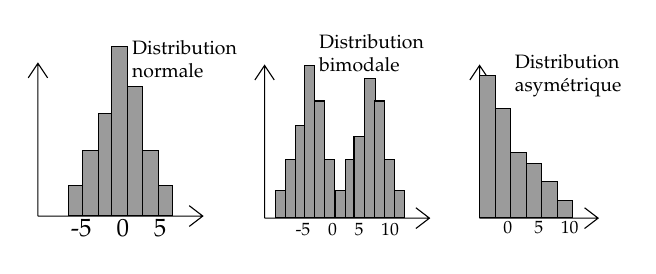
\begin{tikzpicture}[x=0.70pt,y=0.75pt,yscale=-1,xscale=1]
%uncomment if require: \path (0,113.19999694824219); %set diagram left start at 0, and has height of 113.19999694824219

%Shape: Axis 2D [id:dp25296516013925663] 
\draw  (39.32,90.58) -- (124.43,90.58)(39.32,17) -- (39.32,90.58) -- cycle (117.43,85.58) -- (124.43,90.58) -- (117.43,95.58) (34.32,24) -- (39.32,17) -- (44.32,24)  ;
%Shape: Axis 2D [id:dp7734364235695017] 
\draw  (156.32,91.58) -- (241.43,91.58)(156.32,18) -- (156.32,91.58) -- cycle (234.43,86.58) -- (241.43,91.58) -- (234.43,96.58) (151.32,25) -- (156.32,18) -- (161.32,25)  ;
%Shape: Rectangle [id:dp5397609974182909] 
\draw  [fill={rgb, 255:red, 155; green, 155; blue, 155 }  ,fill opacity=1 ] (55,76) -- (62.5,76) -- (62.5,90.2) -- (55,90.2) -- cycle ;
%Shape: Rectangle [id:dp23978833992949755] 
\draw  [fill={rgb, 255:red, 155; green, 155; blue, 155 }  ,fill opacity=1 ] (62.5,59.1) -- (73.5,59.1) -- (73.5,90.2) -- (62.5,90.2) -- cycle ;
%Shape: Rectangle [id:dp03810565350046691] 
\draw  [fill={rgb, 255:red, 155; green, 155; blue, 155 }  ,fill opacity=1 ] (70.5,41) -- (77.5,41) -- (77.5,90.2) -- (70.5,90.2) -- cycle ;
%Shape: Rectangle [id:dp5062656343609877] 
\draw  [fill={rgb, 255:red, 155; green, 155; blue, 155 }  ,fill opacity=1 ] (77.5,9) -- (85.5,9) -- (85.5,90.2) -- (77.5,90.2) -- cycle ;
%Shape: Rectangle [id:dp20312298219270897] 
\draw  [fill={rgb, 255:red, 155; green, 155; blue, 155 }  ,fill opacity=1 ] (85.5,28) -- (93.5,28) -- (93.5,90.2) -- (85.5,90.2) -- cycle ;
%Shape: Rectangle [id:dp08897981680098854] 
\draw  [fill={rgb, 255:red, 155; green, 155; blue, 155 }  ,fill opacity=1 ] (101.5,76) -- (109,76) -- (109,90.2) -- (101.5,90.2) -- cycle ;
%Shape: Rectangle [id:dp5619871752086578] 
\draw  [fill={rgb, 255:red, 155; green, 155; blue, 155 }  ,fill opacity=1 ] (93.5,59.1) -- (101.5,59.1) -- (101.5,90.2) -- (93.5,90.2) -- cycle ;
%Shape: Rectangle [id:dp5892334529757519] 
\draw  [fill={rgb, 255:red, 155; green, 155; blue, 155 }  ,fill opacity=1 ] (162,78.4) -- (166.93,78.4) -- (166.93,91.2) -- (162,91.2) -- cycle ;
%Shape: Rectangle [id:dp31971770319169623] 
\draw  [fill={rgb, 255:red, 155; green, 155; blue, 155 }  ,fill opacity=1 ] (166.93,63.16) -- (174.16,63.16) -- (174.16,91.2) -- (166.93,91.2) -- cycle ;
%Shape: Rectangle [id:dp9378519314749942] 
\draw  [fill={rgb, 255:red, 155; green, 155; blue, 155 }  ,fill opacity=1 ] (172.19,46.85) -- (176.79,46.85) -- (176.79,91.2) -- (172.19,91.2) -- cycle ;
%Shape: Rectangle [id:dp981255335263604] 
\draw  [fill={rgb, 255:red, 155; green, 155; blue, 155 }  ,fill opacity=1 ] (176.79,18) -- (182.05,18) -- (182.05,91.2) -- (176.79,91.2) -- cycle ;
%Shape: Rectangle [id:dp09823668841741062] 
\draw  [fill={rgb, 255:red, 155; green, 155; blue, 155 }  ,fill opacity=1 ] (182.05,35.13) -- (187.31,35.13) -- (187.31,91.2) -- (182.05,91.2) -- cycle ;
%Shape: Rectangle [id:dp9576612819159727] 
\draw  [fill={rgb, 255:red, 155; green, 155; blue, 155 }  ,fill opacity=1 ] (191.57,78.4) -- (196.5,78.4) -- (196.5,91.2) -- (191.57,91.2) -- cycle ;
%Shape: Rectangle [id:dp1999395932653807] 
\draw  [fill={rgb, 255:red, 155; green, 155; blue, 155 }  ,fill opacity=1 ] (187.31,63.16) -- (192.57,63.16) -- (192.57,91.2) -- (187.31,91.2) -- cycle ;
%Shape: Rectangle [id:dp6297327835381095] 
\draw  [fill={rgb, 255:red, 155; green, 155; blue, 155 }  ,fill opacity=1 ] (193,78.4) -- (197.93,78.4) -- (197.93,91.2) -- (193,91.2) -- cycle ;
%Shape: Rectangle [id:dp9951949372205449] 
\draw  [fill={rgb, 255:red, 155; green, 155; blue, 155 }  ,fill opacity=1 ] (197.93,63.16) -- (205.16,63.16) -- (205.16,91.2) -- (197.93,91.2) -- cycle ;
%Shape: Rectangle [id:dp4124751344295785] 
\draw  [fill={rgb, 255:red, 155; green, 155; blue, 155 }  ,fill opacity=1 ] (202.5,52.26) -- (207.79,52.26) -- (207.79,91.2) -- (202.5,91.2) -- cycle ;
%Shape: Rectangle [id:dp8529429794449694] 
\draw  [fill={rgb, 255:red, 155; green, 155; blue, 155 }  ,fill opacity=1 ] (207.79,24.31) -- (213.5,24.31) -- (213.5,91.2) -- (207.79,91.2) -- cycle ;
%Shape: Rectangle [id:dp4911981590320289] 
\draw  [fill={rgb, 255:red, 155; green, 155; blue, 155 }  ,fill opacity=1 ] (213.05,35.13) -- (218.31,35.13) -- (218.31,91.2) -- (213.05,91.2) -- cycle ;
%Shape: Rectangle [id:dp8805884451344097] 
\draw  [fill={rgb, 255:red, 155; green, 155; blue, 155 }  ,fill opacity=1 ] (223.57,78.4) -- (228.5,78.4) -- (228.5,91.2) -- (223.57,91.2) -- cycle ;
%Shape: Rectangle [id:dp602310303075422] 
\draw  [fill={rgb, 255:red, 155; green, 155; blue, 155 }  ,fill opacity=1 ] (218.31,63.16) -- (223.57,63.16) -- (223.57,91.2) -- (218.31,91.2) -- cycle ;
%Shape: Axis 2D [id:dp11205094593877818] 
\draw  (267.32,91.58) -- (328.5,91.58)(267.32,18) -- (267.32,91.58) -- cycle (321.5,86.58) -- (328.5,91.58) -- (321.5,96.58) (262.32,25) -- (267.32,18) -- (272.32,25)  ;
%Shape: Rectangle [id:dp7022940423439525] 
\draw  [fill={rgb, 255:red, 155; green, 155; blue, 155 }  ,fill opacity=1 ] (267.5,23) -- (275.5,23) -- (275.5,91.2) -- (267.5,91.2) -- cycle ;
%Shape: Rectangle [id:dp9865355458935452] 
\draw  [fill={rgb, 255:red, 155; green, 155; blue, 155 }  ,fill opacity=1 ] (275.5,38.96) -- (283.5,38.96) -- (283.5,91.2) -- (275.5,91.2) -- cycle ;
%Shape: Rectangle [id:dp8730759690527732] 
\draw  [fill={rgb, 255:red, 155; green, 155; blue, 155 }  ,fill opacity=1 ] (283.5,60) -- (291.5,60) -- (291.5,91.2) -- (283.5,91.2) -- cycle ;
%Shape: Rectangle [id:dp4068945026575417] 
\draw  [fill={rgb, 255:red, 155; green, 155; blue, 155 }  ,fill opacity=1 ] (307.5,83) -- (315.5,83) -- (315.5,91.2) -- (307.5,91.2) -- cycle ;
%Shape: Rectangle [id:dp9895792370443064] 
\draw  [fill={rgb, 255:red, 155; green, 155; blue, 155 }  ,fill opacity=1 ] (299.5,74) -- (307.5,74) -- (307.5,91.2) -- (299.5,91.2) -- cycle ;
%Shape: Rectangle [id:dp025218688294420533] 
\draw  [fill={rgb, 255:red, 155; green, 155; blue, 155 }  ,fill opacity=1 ] (291.5,65.08) -- (299.5,65.08) -- (299.5,91.2) -- (291.5,91.2) -- cycle ;

% Text Node
\draw (81,96.2) node  [align=left] {{\small -5\ \ \ \ 0\ \ \ \ 5}};
% Text Node
\draw (199,97.2) node [scale=0.8] [align=left] {{\footnotesize -5\ \ \ \ 0\ \ \ \ 5\ \ \ \ 10}};
% Text Node
\draw (299,96.2) node [scale=0.8] [align=left] {{\footnotesize 0 \ \ \ \ 5\ \ \ \ 10}};
% Text Node
\draw (313,22.82) node [scale=0.7] [align=left] {Distribution\\asymétrique};
% Text Node
\draw (211.5,12) node [scale=0.7] [align=left] {Distribution\\bimodale};
% Text Node
\draw (115,14.82) node [scale=0.7] [align=left] {Distribution\\normale};


\end{tikzpicture}
\item Q-Q Plot Normal : les résidus du modèle doivent suivre la droite des quantiles normaux théoriques.


\tikzset{every picture/.style={line width=0.75pt}} %set default line width to 0.75pt        

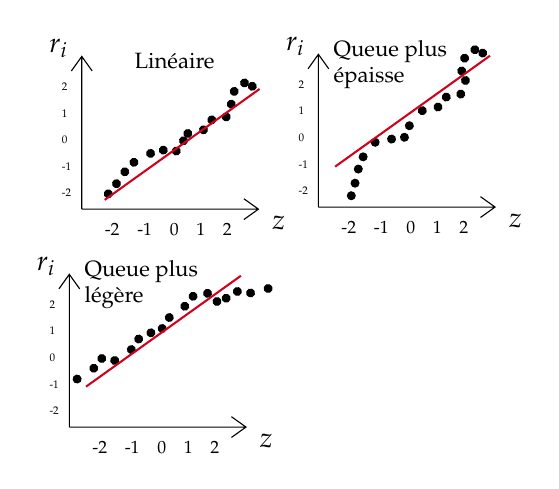
\begin{tikzpicture}[x=0.75pt,y=0.75pt,yscale=-1,xscale=1]
%uncomment if require: \path (0,219.79999923706055); %set diagram left start at 0, and has height of 219.79999923706055

%Shape: Axis 2D [id:dp16254586604443233] 
\draw  (38.32,88.58) -- (123.43,88.58)(38.32,15) -- (38.32,88.58) -- cycle (116.43,83.58) -- (123.43,88.58) -- (116.43,93.58) (33.32,22) -- (38.32,15) -- (43.32,22)  ;
%Flowchart: Connector [id:dp6730588766192098] 
\draw  [fill={rgb, 255:red, 0; green, 0; blue, 0 }  ,fill opacity=1 ] (76.97,61.92) .. controls (75.99,61.58) and (75.47,60.5) .. (75.82,59.52) .. controls (76.16,58.54) and (77.24,58.02) .. (78.22,58.37) .. controls (79.21,58.71) and (79.72,59.79) .. (79.38,60.77) .. controls (79.03,61.75) and (77.95,62.27) .. (76.97,61.92) -- cycle ;
%Flowchart: Connector [id:dp061454342392600614] 
\draw  [fill={rgb, 255:red, 0; green, 0; blue, 0 }  ,fill opacity=1 ] (62.83,67.81) .. controls (61.84,67.46) and (61.33,66.38) .. (61.67,65.4) .. controls (62.02,64.42) and (63.09,63.9) .. (64.08,64.25) .. controls (65.06,64.59) and (65.58,65.67) .. (65.23,66.65) .. controls (64.89,67.64) and (63.81,68.15) .. (62.83,67.81) -- cycle ;
%Flowchart: Connector [id:dp8754614907820837] 
\draw  [fill={rgb, 255:red, 0; green, 0; blue, 0 }  ,fill opacity=1 ] (96.33,52.16) .. controls (95.34,51.81) and (94.83,50.74) .. (95.17,49.75) .. controls (95.52,48.77) and (96.59,48.25) .. (97.58,48.6) .. controls (98.56,48.95) and (99.08,50.02) .. (98.73,51.01) .. controls (98.39,51.99) and (97.31,52.5) .. (96.33,52.16) -- cycle ;
%Flowchart: Connector [id:dp9545215386986239] 
\draw  [fill={rgb, 255:red, 0; green, 0; blue, 0 }  ,fill opacity=1 ] (86.68,57.39) .. controls (85.7,57.05) and (85.18,55.97) .. (85.53,54.99) .. controls (85.87,54.01) and (86.95,53.49) .. (87.93,53.84) .. controls (88.92,54.18) and (89.43,55.26) .. (89.09,56.24) .. controls (88.74,57.22) and (87.67,57.74) .. (86.68,57.39) -- cycle ;
%Flowchart: Connector [id:dp09034585357983449] 
\draw  [fill={rgb, 255:red, 0; green, 0; blue, 0 }  ,fill opacity=1 ] (119.86,31.18) .. controls (118.88,30.84) and (118.36,29.76) .. (118.71,28.78) .. controls (119.05,27.8) and (120.13,27.28) .. (121.11,27.62) .. controls (122.1,27.97) and (122.61,29.05) .. (122.27,30.03) .. controls (121.92,31.01) and (120.85,31.53) .. (119.86,31.18) -- cycle ;
%Flowchart: Connector [id:dp7989698871721915] 
\draw  [fill={rgb, 255:red, 0; green, 0; blue, 0 }  ,fill opacity=1 ] (107.3,45.93) .. controls (106.31,45.58) and (105.8,44.51) .. (106.14,43.52) .. controls (106.49,42.54) and (107.56,42.02) .. (108.55,42.37) .. controls (109.53,42.71) and (110.05,43.79) .. (109.7,44.77) .. controls (109.36,45.76) and (108.28,46.27) .. (107.3,45.93) -- cycle ;
%Flowchart: Connector [id:dp5591290390781647] 
\draw  [fill={rgb, 255:red, 0; green, 0; blue, 0 }  ,fill opacity=1 ] (109.74,39.79) .. controls (108.76,39.44) and (108.24,38.37) .. (108.59,37.38) .. controls (108.93,36.4) and (110.01,35.88) .. (110.99,36.23) .. controls (111.97,36.57) and (112.49,37.65) .. (112.14,38.63) .. controls (111.8,39.62) and (110.72,40.13) .. (109.74,39.79) -- cycle ;
%Flowchart: Connector [id:dp963807309552837] 
\draw  [fill={rgb, 255:red, 0; green, 0; blue, 0 }  ,fill opacity=1 ] (100.32,47.36) .. controls (99.34,47.01) and (98.82,45.93) .. (99.17,44.95) .. controls (99.51,43.97) and (100.59,43.45) .. (101.57,43.8) .. controls (102.56,44.14) and (103.07,45.22) .. (102.73,46.2) .. controls (102.38,47.19) and (101.3,47.7) .. (100.32,47.36) -- cycle ;
%Flowchart: Connector [id:dp7205093809979437] 
\draw  [fill={rgb, 255:red, 0; green, 0; blue, 0 }  ,fill opacity=1 ] (58.44,72.37) .. controls (57.46,72.03) and (56.94,70.95) .. (57.29,69.97) .. controls (57.63,68.99) and (58.71,68.47) .. (59.69,68.82) .. controls (60.68,69.16) and (61.19,70.24) .. (60.85,71.22) .. controls (60.5,72.2) and (59.42,72.72) .. (58.44,72.37) -- cycle ;
%Flowchart: Connector [id:dp125532321132791] 
\draw  [fill={rgb, 255:red, 0; green, 0; blue, 0 }  ,fill opacity=1 ] (70.83,63.51) .. controls (69.85,63.17) and (69.33,62.09) .. (69.68,61.11) .. controls (70.02,60.12) and (71.1,59.61) .. (72.08,59.95) .. controls (73.07,60.3) and (73.58,61.38) .. (73.24,62.36) .. controls (72.89,63.34) and (71.81,63.86) .. (70.83,63.51) -- cycle ;
%Flowchart: Connector [id:dp1953819591243342] 
\draw  [fill={rgb, 255:red, 0; green, 0; blue, 0 }  ,fill opacity=1 ] (54.41,78.08) .. controls (53.43,77.73) and (52.91,76.66) .. (53.26,75.67) .. controls (53.6,74.69) and (54.68,74.18) .. (55.66,74.52) .. controls (56.65,74.87) and (57.16,75.94) .. (56.82,76.93) .. controls (56.47,77.91) and (55.4,78.43) .. (54.41,78.08) -- cycle ;
%Flowchart: Connector [id:dp9983353529614851] 
\draw  [fill={rgb, 255:red, 0; green, 0; blue, 0 }  ,fill opacity=1 ] (83.22,62.37) .. controls (82.24,62.02) and (81.72,60.94) .. (82.07,59.96) .. controls (82.41,58.98) and (83.49,58.46) .. (84.47,58.81) .. controls (85.46,59.15) and (85.97,60.23) .. (85.63,61.21) .. controls (85.28,62.19) and (84.21,62.71) .. (83.22,62.37) -- cycle ;
%Flowchart: Connector [id:dp3531208745847416] 
\draw  [fill={rgb, 255:red, 0; green, 0; blue, 0 }  ,fill opacity=1 ] (88.77,53.91) .. controls (87.78,53.56) and (87.27,52.49) .. (87.61,51.5) .. controls (87.96,50.52) and (89.03,50) .. (90.02,50.35) .. controls (91,50.69) and (91.52,51.77) .. (91.17,52.75) .. controls (90.83,53.74) and (89.75,54.25) .. (88.77,53.91) -- cycle ;
%Flowchart: Connector [id:dp7374531148183092] 
\draw  [fill={rgb, 255:red, 0; green, 0; blue, 0 }  ,fill opacity=1 ] (50.46,82.99) .. controls (49.48,82.64) and (48.96,81.56) .. (49.3,80.58) .. controls (49.65,79.6) and (50.73,79.08) .. (51.71,79.43) .. controls (52.69,79.77) and (53.21,80.85) .. (52.86,81.83) .. controls (52.52,82.81) and (51.44,83.33) .. (50.46,82.99) -- cycle ;
%Flowchart: Connector [id:dp8174464033004614] 
\draw  [fill={rgb, 255:red, 0; green, 0; blue, 0 }  ,fill opacity=1 ] (111.14,33.63) .. controls (110.16,33.29) and (109.65,32.21) .. (109.99,31.23) .. controls (110.34,30.25) and (111.41,29.73) .. (112.4,30.08) .. controls (113.38,30.42) and (113.9,31.5) .. (113.55,32.48) .. controls (113.2,33.46) and (112.13,33.98) .. (111.14,33.63) -- cycle ;
%Flowchart: Connector [id:dp6138703635271334] 
\draw  [fill={rgb, 255:red, 0; green, 0; blue, 0 }  ,fill opacity=1 ] (116.08,29.56) .. controls (115.1,29.21) and (114.58,28.14) .. (114.93,27.15) .. controls (115.27,26.17) and (116.35,25.65) .. (117.33,26) .. controls (118.32,26.34) and (118.83,27.42) .. (118.49,28.4) .. controls (118.14,29.39) and (117.07,29.9) .. (116.08,29.56) -- cycle ;
%Straight Lines [id:da9970832217250101] 
\draw [color={rgb, 255:red, 208; green, 2; blue, 27 }  ,draw opacity=1 ][line width=0.75]    (49.37,84.11) -- (124,30.68) ;


%Shape: Axis 2D [id:dp37439331306989665] 
\draw  (152.32,87.58) -- (237.43,87.58)(152.32,14) -- (152.32,87.58) -- cycle (230.43,82.58) -- (237.43,87.58) -- (230.43,92.58) (147.32,21) -- (152.32,14) -- (157.32,21)  ;
%Flowchart: Connector [id:dp36784388926470934] 
\draw  [fill={rgb, 255:red, 0; green, 0; blue, 0 }  ,fill opacity=1 ] (187.33,56.69) .. controls (186.29,56.55) and (185.57,55.6) .. (185.7,54.57) .. controls (185.84,53.53) and (186.79,52.81) .. (187.82,52.94) .. controls (188.85,53.08) and (189.58,54.03) .. (189.44,55.06) .. controls (189.31,56.1) and (188.36,56.82) .. (187.33,56.69) -- cycle ;
%Flowchart: Connector [id:dp7007733222978385] 
\draw  [fill={rgb, 255:red, 0; green, 0; blue, 0 }  ,fill opacity=1 ] (173.97,65.27) .. controls (172.93,65.32) and (172.04,64.52) .. (171.99,63.48) .. controls (171.94,62.44) and (172.74,61.55) .. (173.78,61.5) .. controls (174.82,61.44) and (175.7,62.25) .. (175.76,63.29) .. controls (175.81,64.33) and (175.01,65.21) .. (173.97,65.27) -- cycle ;
%Flowchart: Connector [id:dp6351646556662804] 
\draw  [fill={rgb, 255:red, 0; green, 0; blue, 0 }  ,fill opacity=1 ] (209.33,41.16) .. controls (208.34,40.81) and (207.83,39.74) .. (208.17,38.75) .. controls (208.52,37.77) and (209.59,37.25) .. (210.58,37.6) .. controls (211.56,37.95) and (212.08,39.02) .. (211.73,40.01) .. controls (211.39,40.99) and (210.31,41.5) .. (209.33,41.16) -- cycle ;
%Flowchart: Connector [id:dp5896633300215095] 
\draw  [fill={rgb, 255:red, 0; green, 0; blue, 0 }  ,fill opacity=1 ] (195.9,50.26) .. controls (194.87,50.13) and (194.15,49.18) .. (194.28,48.14) .. controls (194.42,47.11) and (195.37,46.38) .. (196.4,46.52) .. controls (197.43,46.66) and (198.16,47.61) .. (198.02,48.64) .. controls (197.89,49.67) and (196.94,50.4) .. (195.9,50.26) -- cycle ;
%Flowchart: Connector [id:dp860155333003052] 
\draw  [fill={rgb, 255:red, 0; green, 0; blue, 0 }  ,fill opacity=1 ] (230.86,15.18) .. controls (229.88,14.84) and (229.36,13.76) .. (229.71,12.78) .. controls (230.05,11.8) and (231.13,11.28) .. (232.11,11.62) .. controls (233.1,11.97) and (233.61,13.05) .. (233.27,14.03) .. controls (232.92,15.01) and (231.85,15.53) .. (230.86,15.18) -- cycle ;
%Flowchart: Connector [id:dp7986295850529821] 
\draw  [fill={rgb, 255:red, 0; green, 0; blue, 0 }  ,fill opacity=1 ] (220.3,34.93) .. controls (219.31,34.58) and (218.8,33.51) .. (219.14,32.52) .. controls (219.49,31.54) and (220.56,31.02) .. (221.55,31.37) .. controls (222.53,31.71) and (223.05,32.79) .. (222.7,33.77) .. controls (222.36,34.76) and (221.28,35.27) .. (220.3,34.93) -- cycle ;
%Flowchart: Connector [id:dp035909545346903604] 
\draw  [fill={rgb, 255:red, 0; green, 0; blue, 0 }  ,fill opacity=1 ] (220.74,23.79) .. controls (219.76,23.44) and (219.24,22.37) .. (219.59,21.38) .. controls (219.93,20.4) and (221.01,19.88) .. (221.99,20.23) .. controls (222.97,20.57) and (223.49,21.65) .. (223.14,22.63) .. controls (222.8,23.62) and (221.72,24.13) .. (220.74,23.79) -- cycle ;
%Flowchart: Connector [id:dp3182117437055658] 
\draw  [fill={rgb, 255:red, 0; green, 0; blue, 0 }  ,fill opacity=1 ] (213.32,36.36) .. controls (212.34,36.01) and (211.82,34.93) .. (212.17,33.95) .. controls (212.51,32.97) and (213.59,32.45) .. (214.57,32.8) .. controls (215.56,33.14) and (216.07,34.22) .. (215.73,35.2) .. controls (215.38,36.19) and (214.3,36.7) .. (213.32,36.36) -- cycle ;
%Flowchart: Connector [id:dp44045986632201184] 
\draw  [fill={rgb, 255:red, 0; green, 0; blue, 0 }  ,fill opacity=1 ] (171.64,71.15) .. controls (170.6,71.21) and (169.71,70.4) .. (169.66,69.36) .. controls (169.61,68.32) and (170.41,67.44) .. (171.45,67.38) .. controls (172.49,67.33) and (173.37,68.13) .. (173.43,69.17) .. controls (173.48,70.21) and (172.68,71.1) .. (171.64,71.15) -- cycle ;
%Flowchart: Connector [id:dp432249106030846] 
\draw  [fill={rgb, 255:red, 0; green, 0; blue, 0 }  ,fill opacity=1 ] (179.75,58.26) .. controls (178.71,58.31) and (177.82,57.51) .. (177.77,56.47) .. controls (177.72,55.43) and (178.52,54.54) .. (179.56,54.49) .. controls (180.6,54.44) and (181.49,55.24) .. (181.54,56.28) .. controls (181.59,57.32) and (180.79,58.21) .. (179.75,58.26) -- cycle ;
%Flowchart: Connector [id:dp23417391142862454] 
\draw  [fill={rgb, 255:red, 0; green, 0; blue, 0 }  ,fill opacity=1 ] (170.07,77.96) .. controls (169.03,78.01) and (168.14,77.21) .. (168.09,76.17) .. controls (168.04,75.13) and (168.84,74.24) .. (169.88,74.19) .. controls (170.92,74.14) and (171.81,74.94) .. (171.86,75.98) .. controls (171.91,77.02) and (171.11,77.91) .. (170.07,77.96) -- cycle ;
%Flowchart: Connector [id:dp12664418911817132] 
\draw  [fill={rgb, 255:red, 0; green, 0; blue, 0 }  ,fill opacity=1 ] (193.54,55.84) .. controls (192.5,55.7) and (191.78,54.75) .. (191.91,53.72) .. controls (192.05,52.68) and (193,51.96) .. (194.03,52.1) .. controls (195.06,52.23) and (195.79,53.18) .. (195.65,54.21) .. controls (195.52,55.25) and (194.57,55.97) .. (193.54,55.84) -- cycle ;
%Flowchart: Connector [id:dp5161152629757335] 
\draw  [fill={rgb, 255:red, 0; green, 0; blue, 0 }  ,fill opacity=1 ] (201.77,42.91) .. controls (200.78,42.56) and (200.27,41.49) .. (200.61,40.5) .. controls (200.96,39.52) and (202.03,39) .. (203.02,39.35) .. controls (204,39.69) and (204.52,40.77) .. (204.17,41.75) .. controls (203.83,42.74) and (202.75,43.25) .. (201.77,42.91) -- cycle ;
%Flowchart: Connector [id:dp016809776436435886] 
\draw  [fill={rgb, 255:red, 0; green, 0; blue, 0 }  ,fill opacity=1 ] (168.27,84) .. controls (167.23,84.05) and (166.34,83.25) .. (166.29,82.21) .. controls (166.24,81.17) and (167.04,80.28) .. (168.08,80.23) .. controls (169.12,80.18) and (170,80.98) .. (170.06,82.02) .. controls (170.11,83.06) and (169.31,83.94) .. (168.27,84) -- cycle ;
%Flowchart: Connector [id:dp5174795408171224] 
\draw  [fill={rgb, 255:red, 0; green, 0; blue, 0 }  ,fill opacity=1 ] (222.14,17.63) .. controls (221.16,17.29) and (220.65,16.21) .. (220.99,15.23) .. controls (221.34,14.25) and (222.41,13.73) .. (223.4,14.08) .. controls (224.38,14.42) and (224.9,15.5) .. (224.55,16.48) .. controls (224.2,17.46) and (223.13,17.98) .. (222.14,17.63) -- cycle ;
%Flowchart: Connector [id:dp5631080940724282] 
\draw  [fill={rgb, 255:red, 0; green, 0; blue, 0 }  ,fill opacity=1 ] (227.08,13.56) .. controls (226.1,13.21) and (225.58,12.14) .. (225.93,11.15) .. controls (226.27,10.17) and (227.35,9.65) .. (228.33,10) .. controls (229.32,10.34) and (229.83,11.42) .. (229.49,12.4) .. controls (229.14,13.39) and (228.07,13.9) .. (227.08,13.56) -- cycle ;
%Straight Lines [id:da2946368899193359] 
\draw [color={rgb, 255:red, 208; green, 2; blue, 27 }  ,draw opacity=1 ][line width=0.75]    (160.37,68.11) -- (229.13,18.88) -- (235,14.68) ;


%Flowchart: Connector [id:dp7440829748354494] 
\draw  [fill={rgb, 255:red, 0; green, 0; blue, 0 }  ,fill opacity=1 ] (222.55,28.37) .. controls (221.56,28.02) and (221.05,26.95) .. (221.39,25.96) .. controls (221.74,24.98) and (222.82,24.46) .. (223.8,24.81) .. controls (224.78,25.16) and (225.3,26.23) .. (224.95,27.22) .. controls (224.61,28.2) and (223.53,28.71) .. (222.55,28.37) -- cycle ;

%Shape: Axis 2D [id:dp7757599245408202] 
\draw  (32.32,193.58) -- (117.43,193.58)(32.32,120) -- (32.32,193.58) -- cycle (110.43,188.58) -- (117.43,193.58) -- (110.43,198.58) (27.32,127) -- (32.32,120) -- (37.32,127)  ;
%Flowchart: Connector [id:dp9445375746382854] 
\draw  [fill={rgb, 255:red, 0; green, 0; blue, 0 }  ,fill opacity=1 ] (54.93,159.77) .. controls (55.88,160.2) and (56.31,161.31) .. (55.88,162.27) .. controls (55.46,163.22) and (54.35,163.65) .. (53.39,163.22) .. controls (52.44,162.8) and (52.01,161.68) .. (52.44,160.73) .. controls (52.86,159.78) and (53.97,159.35) .. (54.93,159.77) -- cycle ;
%Flowchart: Connector [id:dp6929609208327578] 
\draw  [fill={rgb, 255:red, 0; green, 0; blue, 0 }  ,fill opacity=1 ] (66.17,149.32) .. controls (67.18,149.57) and (67.8,150.58) .. (67.56,151.6) .. controls (67.32,152.61) and (66.3,153.23) .. (65.28,152.99) .. controls (64.27,152.75) and (63.65,151.73) .. (63.89,150.71) .. controls (64.13,149.7) and (65.15,149.08) .. (66.17,149.32) -- cycle ;
%Flowchart: Connector [id:dp25988018614492314] 
\draw  [fill={rgb, 255:red, 0; green, 0; blue, 0 }  ,fill opacity=1 ] (87.33,137.16) .. controls (86.34,136.81) and (85.83,135.74) .. (86.17,134.75) .. controls (86.52,133.77) and (87.59,133.25) .. (88.58,133.6) .. controls (89.56,133.95) and (90.08,135.02) .. (89.73,136.01) .. controls (89.39,136.99) and (88.31,137.5) .. (87.33,137.16) -- cycle ;
%Flowchart: Connector [id:dp5342956162739945] 
\draw  [fill={rgb, 255:red, 0; green, 0; blue, 0 }  ,fill opacity=1 ] (44.88,163.51) .. controls (45.83,163.93) and (46.26,165.05) .. (45.84,166) .. controls (45.42,166.95) and (44.3,167.38) .. (43.35,166.96) .. controls (42.4,166.54) and (41.97,165.42) .. (42.39,164.47) .. controls (42.82,163.52) and (43.93,163.09) .. (44.88,163.51) -- cycle ;
%Flowchart: Connector [id:dp4912190099730125] 
\draw  [fill={rgb, 255:red, 0; green, 0; blue, 0 }  ,fill opacity=1 ] (126.39,127.6) .. controls (125.95,126.65) and (126.37,125.53) .. (127.32,125.1) .. controls (128.26,124.67) and (129.38,125.08) .. (129.82,126.03) .. controls (130.25,126.98) and (129.83,128.1) .. (128.89,128.53) .. controls (127.94,128.96) and (126.82,128.55) .. (126.39,127.6) -- cycle ;
%Flowchart: Connector [id:dp9388549352873456] 
\draw  [fill={rgb, 255:red, 0; green, 0; blue, 0 }  ,fill opacity=1 ] (98.3,130.93) .. controls (97.31,130.58) and (96.8,129.51) .. (97.14,128.52) .. controls (97.49,127.54) and (98.56,127.02) .. (99.55,127.37) .. controls (100.53,127.71) and (101.05,128.79) .. (100.7,129.77) .. controls (100.36,130.76) and (99.28,131.27) .. (98.3,130.93) -- cycle ;
%Flowchart: Connector [id:dp9774342140320689] 
\draw  [fill={rgb, 255:red, 0; green, 0; blue, 0 }  ,fill opacity=1 ] (106.16,132.29) .. controls (105.73,131.34) and (106.15,130.22) .. (107.09,129.79) .. controls (108.04,129.35) and (109.16,129.77) .. (109.59,130.72) .. controls (110.03,131.66) and (109.61,132.78) .. (108.66,133.22) .. controls (107.72,133.65) and (106.6,133.23) .. (106.16,132.29) -- cycle ;
%Flowchart: Connector [id:dp7316467394936874] 
\draw  [fill={rgb, 255:red, 0; green, 0; blue, 0 }  ,fill opacity=1 ] (91.32,132.36) .. controls (90.34,132.01) and (89.82,130.93) .. (90.17,129.95) .. controls (90.51,128.97) and (91.59,128.45) .. (92.57,128.8) .. controls (93.56,129.14) and (94.07,130.22) .. (93.73,131.2) .. controls (93.38,132.19) and (92.3,132.7) .. (91.32,132.36) -- cycle ;
%Flowchart: Connector [id:dp21883994035641696] 
\draw  [fill={rgb, 255:red, 0; green, 0; blue, 0 }  ,fill opacity=1 ] (72.07,146.33) .. controls (73.08,146.58) and (73.7,147.59) .. (73.46,148.61) .. controls (73.21,149.62) and (72.19,150.24) .. (71.18,150) .. controls (70.17,149.76) and (69.55,148.74) .. (69.79,147.72) .. controls (70.03,146.71) and (71.05,146.09) .. (72.07,146.33) -- cycle ;
%Flowchart: Connector [id:dp24376162755606323] 
\draw  [fill={rgb, 255:red, 0; green, 0; blue, 0 }  ,fill opacity=1 ] (62.64,154.41) .. controls (63.65,154.65) and (64.28,155.67) .. (64.03,156.68) .. controls (63.79,157.7) and (62.77,158.32) .. (61.76,158.07) .. controls (60.74,157.83) and (60.12,156.81) .. (60.36,155.8) .. controls (60.61,154.79) and (61.63,154.16) .. (62.64,154.41) -- cycle ;
%Flowchart: Connector [id:dp3413228173778866] 
\draw  [fill={rgb, 255:red, 0; green, 0; blue, 0 }  ,fill opacity=1 ] (77.49,144.25) .. controls (78.51,144.49) and (79.13,145.51) .. (78.88,146.52) .. controls (78.64,147.54) and (77.62,148.16) .. (76.61,147.92) .. controls (75.6,147.67) and (74.97,146.65) .. (75.22,145.64) .. controls (75.46,144.63) and (76.48,144) .. (77.49,144.25) -- cycle ;
%Flowchart: Connector [id:dp2547933050624429] 
\draw  [fill={rgb, 255:red, 0; green, 0; blue, 0 }  ,fill opacity=1 ] (48.73,158.83) .. controls (49.68,159.26) and (50.11,160.37) .. (49.69,161.33) .. controls (49.26,162.28) and (48.15,162.71) .. (47.2,162.28) .. controls (46.25,161.86) and (45.82,160.74) .. (46.24,159.79) .. controls (46.66,158.84) and (47.78,158.41) .. (48.73,158.83) -- cycle ;
%Flowchart: Connector [id:dp7325135086953662] 
\draw  [fill={rgb, 255:red, 0; green, 0; blue, 0 }  ,fill opacity=1 ] (37.18,168.91) .. controls (38.03,169.52) and (38.22,170.7) .. (37.61,171.54) .. controls (37,172.39) and (35.82,172.58) .. (34.97,171.97) .. controls (34.13,171.36) and (33.94,170.18) .. (34.55,169.34) .. controls (35.16,168.49) and (36.34,168.3) .. (37.18,168.91) -- cycle ;
%Flowchart: Connector [id:dp46250671746845295] 
\draw  [fill={rgb, 255:red, 0; green, 0; blue, 0 }  ,fill opacity=1 ] (80.93,138.97) .. controls (81.94,139.21) and (82.57,140.23) .. (82.32,141.24) .. controls (82.08,142.25) and (81.06,142.88) .. (80.05,142.63) .. controls (79.03,142.39) and (78.41,141.37) .. (78.65,140.36) .. controls (78.9,139.35) and (79.92,138.72) .. (80.93,138.97) -- cycle ;
%Flowchart: Connector [id:dp910576718385065] 
\draw  [fill={rgb, 255:red, 0; green, 0; blue, 0 }  ,fill opacity=1 ] (111.57,129.03) .. controls (111.14,128.08) and (111.55,126.96) .. (112.5,126.53) .. controls (113.45,126.09) and (114.57,126.51) .. (115,127.46) .. controls (115.43,128.4) and (115.02,129.52) .. (114.07,129.96) .. controls (113.12,130.39) and (112,129.97) .. (111.57,129.03) -- cycle ;
%Flowchart: Connector [id:dp2586768703871727] 
\draw  [fill={rgb, 255:red, 0; green, 0; blue, 0 }  ,fill opacity=1 ] (117.93,129.75) .. controls (117.5,128.8) and (117.91,127.68) .. (118.86,127.25) .. controls (119.81,126.82) and (120.93,127.23) .. (121.36,128.18) .. controls (121.8,129.13) and (121.38,130.25) .. (120.43,130.68) .. controls (119.48,131.12) and (118.37,130.7) .. (117.93,129.75) -- cycle ;
%Straight Lines [id:da26641821072648253] 
\draw [color={rgb, 255:red, 208; green, 2; blue, 27 }  ,draw opacity=1 ][line width=0.75]    (40.37,174.11) -- (109.13,124.88) -- (115,120.68) ;


%Flowchart: Connector [id:dp3900800225512009] 
\draw  [fill={rgb, 255:red, 0; green, 0; blue, 0 }  ,fill opacity=1 ] (101.73,133.86) .. controls (101.3,132.91) and (101.72,131.79) .. (102.66,131.36) .. controls (103.61,130.92) and (104.73,131.34) .. (105.16,132.29) .. controls (105.6,133.23) and (105.18,134.35) .. (104.23,134.79) .. controls (103.29,135.22) and (102.17,134.8) .. (101.73,133.86) -- cycle ;

% Text Node
\draw (27.26,11.18) node  [align=left] {$\displaystyle r_{i}$};
% Text Node
\draw (83,17) node [scale=0.8] [align=left] {Linéaire};
% Text Node
\draw (133.26,95.18) node  [align=left] {$\displaystyle z$};
% Text Node
\draw (80,98.2) node [scale=0.8] [align=left] {{\footnotesize -2 \ \ \ -1 \ \ \ 0 \ \ \ 1 \ \ \ 2}};
% Text Node
\draw (31,55.2) node [scale=0.8] [align=left] {{\tiny 2}\\{\tiny 1}\\{\tiny 0}\\{\tiny -1}\\{\tiny -2}};
% Text Node
\draw (141.26,10.18) node  [align=left] {$\displaystyle r_{i}$};
% Text Node
\draw (187,19) node [scale=0.8] [align=left] {Queue plus \\épaisse};
% Text Node
\draw (247.26,94.18) node  [align=left] {$\displaystyle z$};
% Text Node
\draw (194,97.2) node [scale=0.8] [align=left] {{\footnotesize -2 \ \ \ -1 \ \ \ 0 \ \ \ 1 \ \ \ 2}};
% Text Node
\draw (145,54.2) node [scale=0.8] [align=left] {{\tiny 2}\\{\tiny 1}\\{\tiny 0}\\{\tiny -1}\\{\tiny -2}};
% Text Node
\draw (21.26,116.18) node  [align=left] {$\displaystyle r_{i}$};
% Text Node
\draw (67,125) node [scale=0.8] [align=left] {Queue plus \\légère};
% Text Node
\draw (127.26,200.18) node  [align=left] {$\displaystyle z$};
% Text Node
\draw (74,203.2) node [scale=0.8] [align=left] {{\footnotesize -2 \ \ \ -1 \ \ \ 0 \ \ \ 1 \ \ \ 2}};
% Text Node
\draw (25,160.2) node [scale=0.8] [align=left] {{\tiny 2}\\{\tiny 1}\\{\tiny 0}\\{\tiny -1}\\{\tiny -2}};


\end{tikzpicture}


\end{itemize}

\subsection*{Transformation des données}
\begin{enumerate}
	\item $V(\epsilon_i) \propto \esp{Y_i}$ et les données de type Poisson.
	\[g(Y) = \sqrt{Y}\]
	\item $V(\epsilon_i) \propto (\esp{Y_i})^2$ avec la situation la plus efficace étant si $Y$ possède une très grande étendue.
	\[g(Y) = log(Y)\]
	\item $V(\epsilon_i) \propto (\esp{Y_i})^4$. 
	\[g(Y) = 1/Y\]
	\item $V(\epsilon_i) \propto \esp{Y_i}(1 - \esp{Y_i})$, $Y \in [0, 1]$ et $Y \sim \text{Bern}$. 
	\[g(Y) = \text{arcsin}(\sqrt{Y})\]
\end{enumerate}

%\vfill\null
\subsection*{Prévision sous transformation}
$\esp{g(Y)} \not = g(\esp{Y})$
\begin{enumerate}
	\item[] Soit une transformation $g(Y) \in [a, b]$
	\item[] En appliquant la transformation inverse, on peut trouver un intervalle pour $Y\in [g^{-1}(a), g^{-1}(b)]$.
\end{enumerate}
Alias, le théorème de la fonction quantile pour une fonction monotone:
\begin{align*}
	\text{Pr}(a \le g(Y) \le b) &= \text{Pr}(g^{-1}(a) \le Y \le g^{-1}(b)) 
\end{align*}


\section{Régression linéaire multiple}
% \mathrm{•} utilise la notation matricielle
% \bm{•} est utilisé pour la notation matricielle, mais lorsqu'il y a des symboles mathématiques.
\subsection*{Le modèle et ses propriétés}
\begin{align*}
\matr{Y}_{n \times 1} &= \matr{X}_{n \times p'} \bm{\beta}_{p' \times 1} + \bm{\varepsilon}_{n \times 1} \\
\esp{\matr{Y}}	&= \matr{X} \bm{\beta} \\
\text{V}({\matr{Y}}) &= \sigma^2 \matr{I}_{n \times n} \\
Y &\overset{H_4}{\sim} \mathcal{N}_n(\matr{X} \bm{\beta}, \sigma^2 \matr{I}_{n \times n}) \\
\end{align*}

\textbf{Matrice d'incidence}\\
\[
\underset{n\times 1}{\underbrace{\begin{pmatrix}
Y_1\\ 
Y_2\\ 
\vdots\\ 
Y_n\\ 
\end{pmatrix}
}}
=
\underset{n\times p'}{\underbrace{\begin{pmatrix}
1 & x_{11} & x_{12} & \dots & x_{1p} \\ 
1 & x_{21} & x_{22} & \dots  & x_{2p} \\ 
\vdots & \vdots & \vdots  & \ddots & \vdots \\ 
1 & x_{n1}  & \dots & x_{np} & x_{np}
\end{pmatrix}}}
\underset{p'\times 1}{\underbrace{\begin{pmatrix}
\beta_1\\ 
\beta_2\\ 
\vdots\\ 
\beta_p\\ 
\end{pmatrix}}}
+
\underset{n\times 1}{\underbrace{\begin{pmatrix}
\epsilon_1\\ 
\epsilon_2\\ 
\vdots\\ 
\epsilon_n\\ 
\end{pmatrix}}}
\]
\\
Types de variables exogènes possible:
\begin{enumerate}
	\item[ - ] \textbf{Dichotomiques} e.g.: présence / absence.
	\item[ - ] \textbf{Discrètes} e.g.: une classe de revenu.
	\item[ - ] \textbf{Continues} e.g.: le poids d'une personne.
	\item[ - ] \textbf{Qualitatives}	e.g.: le sexe.
\end{enumerate}



\subsection*{Paramètres du modèle}
\subsubsection*{Estimation et propriétés des paramètres}
\begin{align*}
\hat{\bm{\beta}} &= \overset{\text{"}S_{XX}\text{"}}{\overbrace{(\matr{X^\top X)^{-1}}}} \overset{\text{"}S_{XY}\text{"}}{\overbrace{\matr{X^\top Y}}} \\
\esp{\hat{\bm{\beta}}}	&= \bm{\beta} \quad \\ Var(\hat{\bm{\beta}}) &= \sigma^2 (\matr{X^\top X)^{-1}} \\
\hat{\bm{\beta}} &\overset{H_4}{\sim} \mathcal{N}_p(\bm{\beta}, \sigma^2 (\matr{X^\top X)^{-1}})
\end{align*}

\subsubsection*{Intervalle de confiance sur les paramètres}
\begin{align*}
&\text{V}(\beta_j) = \sigma^2 v_{jj} \\
&\beta_j \in \left[ \hat{\beta_j} \pm t_{n-p'} \left(1- \frac{\alpha}{2} \right) \sqrt{s^2 v_{jj}} \right]
\end{align*}
où $v_{jj}$ est l'élément $(j,j)$ de la matrice $\matr{(X^\top X)^{-1}}$.

\subsubsection*{Estimation de $\sigma^2$}
%Il peut être démontré que cet estimateur est sans biais et indépendant de $\bm{\hat{\beta}}$.
À noter que $s^{2}\bot \bm{\beta}$ et le $\text{Biais}(s^{2}) = 0$.\\
\begin{align*}
s^2 &= \frac{\hat{\bm{\varepsilon}}^\top \hat{\bm{\varepsilon}}}{n-p'} &\text{où } \frac{\bm{\hat\epsilon}^{\top}\bm{\hat\epsilon}}{\sigma^{2}} &\sim \chi^{2}_{n - p'}
\end{align*}

\subsubsection*{Test d'hypothèse sur un paramètre du modèle}
On rejète $H_0 : \beta_j = 0$ si
\begin{align*}
|t_{obs, j}| = \frac{\beta_j}{\sqrt{s^2 v_{jj}} } > t_{n-p'}\left(1 - \frac{\alpha}{2} \right) 
\end{align*}

\subsection*{Propriétés de la droite de régression}
\begin{align*}
\hat{\matr{Y}} 
	&= \matr{X} \bm{\hat{\beta}}  &
\hat{\varepsilon} 
	&= \matr{Y} - \hat{\matr{Y}} \\
	&= \matr{X(X^\top X)^{-1} X^\top Y} &
	&= (\matr{I}_n - \matr{X(X^\top X)^{-1} X^\top Y}) \\
	&= \matr{H Y}  &
	&= (\matr{I}_n - \matr{H})\matr{Y} 
\end{align*}	
où $\matr{H = X(X^\top X)^{-1}X^\top}$ est la \textit{hat matrix}.\\

On a aussi que
\begin{align*}
\esp{\hat{\matr{Y}}} &= \matr{X} \bm{\beta} & 
\text{V}(\hat{\matr{Y}}) &= \sigma^2 \matr{H} \\
\hat{\matr{Y}} &\overset{H_4}{\sim} N_n(\matr{X} \bm{\beta} , \sigma^2 \matr{H})\\
\end{align*}

Pour les résidus de la droite de régression, on a
\begin{align*}
\esp{\hat{\bm{\varepsilon}}} &\overset{H_1}{=} 0 & 
\text{V}(\hat{\bm{\varepsilon}}) &= \sigma^2(\matr{I}_{n} - \matr{H}) \\
\hat{\bm{\varepsilon}} &\overset{H_4}{\sim} \mathcal{N}_n(0, \sigma^2 (\matr{I}_{n} - \matr{H})) 
\end{align*}

\subsection*{Matrice de projection}
Les matrices $\matr{H}$ et $\matr{I_n - H}$ peuvent être vues commes des matrices de projection. Ces deux opérateurs possèdent plusieurs propriétés:
\begin{enumerate}
	\item $\matr{H}^\top = \matr{H}\:$(symétrie)
	\item $\matr{H}\matr{H} = \matr{H}\:$(idempotence)
	\item $\matr{HX} = \matr{X}$
	\item $(\matr{I}_n - \matr{H}) = (\matr{I}_n - \matr{H})^\top \:$(symétrie)
	\item $(\matr{I}_n - \matr{H})(\matr{I}_n - \matr{H}) = (\matr{I}_n - \matr{H})$
	\item $(\matr{I}_n - \matr{H})\matr{X} = 0 $
	\item $(\matr{I}_n - \matr{H})\matr{H} = 0 $
\end{enumerate}

\subsection*{Intervalle de confiance pour la prévision}
\subsubsection*{Théorème de Gauss-Markov}
Selon les postulats $H_1$ à $H_4$, l'estimateur
\begin{align*}
\mathrm{a^\top} \hat{\bm{\beta}} 
&= \matr{a^\top (X^\top X)^{-1} X^\top Y}\\
&\sim \mathcal{N}(\matr{a^\top} \bm{\beta}, \sigma^{2}\matr{a^\top(X^\top X)^{-1}a})
\end{align*}
est le meilleur estimateur pour $\matr{a^\top} \bm{\beta}$ où $\matr{a^\top} = \matr{c^\top} \bm{X} $ 

(\textbf{BLUE} : Best linear unbiaised estimator).

\subsubsection*{I.C. pour la prévision de la valeur moyenne $\esp{\matr{Y} | \matr{x^*}}$}
\begin{align*}
\left[ \matr{{x^*}^\top} \hat{\bm{\beta}} \pm t_{(n-p'), \alpha/2} \sqrt{s^2 \matr{{x^*}^\top} (\matr{X}^\top \matr{X})^{-1}\matr{x^*}} \right]
\end{align*}

\subsubsection*{I.C. pour la valeur prédite $\hat{\matr{Y}}|\matr{x^*}$}
\begin{align*}
\left[ \matr{{x^*}^\top} \hat{\bm{\beta}} \pm t_{(n-p'), \alpha/2} \sqrt{s^2\left( {\color{blue}1} +  \matr{{x^*}^\top} (\matr{X}^\top \matr{X})^{-1}\matr{x^*}\right)} \right]
\end{align*}


\subsection*{Analyse de la variance}
\subsubsection*{Tableau ANOVA}
\begin{itemize}
\item On utilise le même tableau ANOVA qu'en régression linéaire simple.
\item $SSR_{\text{régression}} = \sum_{i=1}^{p} SSR_i $, où $SSR_i$ représente le SSR individuel de la variable explicative $i$ calculé par R. On peut ensuite trouver $MSR$ et la statistique $F_{obs}$.
\item $SSR(x)$ SSR pour le modèle incluant la variable $x$.
\end{itemize}

\subsubsection*{Test F pour la validité globale de la régression}
Même test qu'en régression linéaire simple.


\subsubsection*{Test F partiel pour la réduction du modèle}
Avec $k < p$, on va rejeter le modèle réduit:
\begin{align*}
H_0 : Y_i &= \beta_0 + \beta_1 x_{i1} + ... + \beta_{ik} x_{ik} + \epsilon_i 
\end{align*}
Pour le modèle complet:
\begin{align*}
H_1 : Y_i &= \beta_0 + \beta_1 x_{i1} + ... \beta_{ip} x_{ip} + \epsilon_i 
\end{align*}
Si
\begin{align*}
F_{obs} = \frac{(SSE^{(0)} - SSE^{(1)}) / \Delta dl}{SSE^{(1)} / (n-p')} \geq F_{p-k, n-p'}(1- \alpha)
\end{align*}
où:
\begin{enumerate}
	\item[] $\Delta dl = p - k$.
	\item[] $SSE^{(0)}$ pour le modèle réduit ($H_0$)
	\item[] $SSE^{(1)}$ pour le modèle complet ($H_1$)
\end{enumerate}

À noter que $\because SST^{(0)} = SST^{(1)} \therefore$
\[
	F_{obs} \Leftrightarrow \frac{(SSR^{(1)} - SSR^{(0)})}{\Delta dl \  MSE^{(1)}}
\]

\subsection*{Régression avec variables qualitatives}

Lorsque nous avons une variable exogène représentant des catégories, il est important de la coder sous forme d'indicatrice:

\begin{align*}
	x_{i} &= \left\{
	\begin{matrix}
		1, & \text{si}\dots \\
		0, & \text{sinon}
	\end{matrix}
	\right.
\end{align*}

Lorsqu'il y a n $\ge 2$ états, alors il faut créer \textbf{n - 1} variables indicatrices.\\
C'est \textbf{n - 1} puisque le n$^{\text{ème}}$ état est représenté lorsque toutes les autres variables indicatrices sont à 0.\\
Exemple avec 3 états \textit{(rouge, bleu, vert)}.
\begin{align*}
	x_{i1} &= \left\{
	\begin{matrix}
		1, & \text{si rouge} \\
		0, & \text{sinon}
	\end{matrix}
	\right.\\
	x_{i2} &= \left\{
	\begin{matrix}
		1, & \text{si bleu} \\
		0, & \text{sinon}
	\end{matrix}
	\right.\\
	x_{i3} &= \left\{
	\begin{matrix}
		1, & \text{si vert} \\
		0, & \text{sinon}
	\end{matrix}
	\right.\\ 
\end{align*}

\textit{\textbf{compléter cette section}}

\subsection*{Multicollinéarité}
Soit une combinaison de constantes \textit{(pas toutes égales à 0} $d_{1}, \dots, d_{p}$.
\begin{description}
	\item[Multicolinéarité \textit{exacte}] Une variable est la combinaison linéaire d'une, \textit{ou plusieurs}, autres variables.\\
	$\sum_{j = 1}^{p}d_{j}X_{j} = 0$
	\item[Multicolinéarité \textit{au sens large}] Lorsqu'une variable est \textit{presque} la combinaison linéaire d'une, ou plusieurs, autres variables.\\
	Plus fréquente et difficile à détecter. \\
	$\sum_{j = 1}^{p}d_{j}X_{j} \approx 0$
\end{description}

\subsubsection*{Problèmes potentiels}
\begin{itemize}
\item Instabilité de $\mathrm{(X^\top X)^{-1}}$, i.e. une petite variation de $Y$ peut causer de grandes variations en $\hat{\beta}$ et $\hat{Y}$.
\item $\hat{\beta}_i$ de signes contre-intuitif.\\
 Pour exemple, le taux de chômage avec $\hat{\beta}_i > 0$ et le taux d'emploi avec $\hat{\beta}_k < 0$.
\item $\text{V}(\hat{\beta}_i)$ et $\text{V}(\hat{Y})$ très grandes.
\item Les méthodes de sélection de variable ne concordent pas.
\item Conclusions erronées sur la significativité de certains paramètres, malgré une forte corrélation avec $Y$.
\end{itemize}

%\vfill\null

\subsubsection*{Détection}
\begin{itemize}
\item Si $r_{ij}$ dans la matrice des coefficients de corrélation échantillonnaux $\matr{{X^*}^\top X^*}$ est élevée, où $\forall j,k \in \{1, \dots, p\}$.

\begin{align*}
\matr{X^{*\top}X^{*}} &= 
	\begin{bmatrix}
		1	&	r_{12}	&	\dots	&	r_{1p}	\\
		r_{21}	&	1	&	\dots	&	r_{2p}	\\
		\vdots	&	\vdots	&	\ddots	&	\vdots	\\
		r_{p1}	&	r_{p2}	&	\dots	&	1	\\		
	\end{bmatrix}_{p \times p} \\
\matr{X^*} &= 
	\begin{bmatrix}
		\frac{x_1 - \bar{x}_1}{s_1} & \dots & \frac{x_p - \bar{x}_p}{s_p}
	\end{bmatrix}_{1 \times p} \\
r_{jk} &= \sum_{i = 1}^{n}\frac{(x_{ji} - \bar{x}_{j})(x_{ki} - \bar{x}_{k})}{s_{j}s_{k}} 
\end{align*}
\item Si le facteur d'inflation de la variance ($VIF_j$) est élevé où:
\begin{align*}
VIF_j = \frac{1}{1 - R_j^2}
\end{align*}
\item[$VIF_j$ :] Pour évaluer le degré de dépendance de chaque variable exogène sur les autres variables exogènes.\\
Pour la $j$\up{e} variable exogène ($x_j$), on mesure le niveau de dépendance en effectuant une régression ayant $x_j$ comme variable explicative (\textit{endogène}) et les $(p - 1)$ variables restantes comme variables explicatives (\textit{exogènes}).\\
$R_j^2$ mesurera la proportion de la variabilité de $x_j$ expliquée par les autres variables explicatives, s'il est élevé il semblerait avoir un problème.\\
Le nom "\textit{facteur d'inflation}" vient du fait que la variance de $\hat{\beta}_j$ s'exprime en fonction du VIF :
\begin{align*}
%	\text{V}(\hat{\beta}_j) = \frac{\sigma^2}{(\matr{X^{*\top} \matr{X^*})_{jj}}} VIF_j
	\text{V}(\hat{\beta}_j) = \frac{\sigma^2}{\sum_{i = 1}^{n}(x_{ij} - \bar{x}_{j})^{2}} VIF_j
\end{align*}
\end{itemize}

\subsubsection*{Solution}
\begin{itemize}
	\item On retire les variables ayant un VIF élevé (une à la fois).
	\item On combine des variables exogènes redondantes	
\end{itemize}

\textbf{Problèmes et détails}
\begin{itemize}
	\item Généralement, on peut considérer un VIF $> 10$ comme un point ou considérer la présence de la multicolinéarité.
	\item Incapable de détecter des mutlicolinéarités de la colonne de 1.
	\item Incapable de cerner le nombre de \textit{quasi} dépendances linéaires dans les données.
	\item Incapable de pointer une valeur précise du VIF où l'on doit vraiment commencer à s'inquiéter (10 est une valeur \textit{ad hoc}).
\end{itemize}

\subsection*{Validation du modèle et des postulats}
\subsubsection*{Linéarité}
\begin{itemize}
\item On trace les \textbf{graphiques à variable ajoutée} ( $\hat{\varepsilon}_{\matr{Y} | \matr{X_{-j}}}$ en fonction de $\hat{\varepsilon}_{x_j | \matr{X_{-j}}}$).
\begin{description}
	\item[$\hat{\varepsilon}_{\matr{Y} | \matr{X_{-j}}}$: ] Vecteur des résidus de la régression de $\matr{Y}$ sur toutes les variables sauf $\matr{x}_{j}$.
	\item[$\hat{\varepsilon}_{x_j | \matr{X_{-j}}}$: ] Vecteur des résidus de la régression avec $\matr{x}_j$ comme variable endogène sur toutes les autres variables exogènes.
\end{description}
\item Ces graphiques doivent normalement donner une droite de pente $\beta_j$.
\begin{itemize}
	\item Si le graphique ressemble à un graphique de résidus normaux, $x_j$ est \textbf{inutile}.
	\item Si il y a une courbe, $x_j$ est \textbf{non-linéaire}.
\end{itemize}
\end{itemize}

\subsubsection*{Homogénéité des variances}
\begin{itemize}
\item Graphique $r_i | \hat{Y}_i$
\end{itemize}

\subsubsection*{Normalité des erreurs}

\begin{itemize}
\item Graphique Q-Q plot normal.
\end{itemize}

\subsubsection*{Indépendance entre les observations}
\begin{itemize}
\item Graphique $\hat{\varepsilon}_i | i$
\item Test de Durbin-Watson pour détecter la présence d'autocorrélation positive entres les résdius.
\item S'il y a autocorrélation, alors $\text{V}(\epsilon) \not= \sigma^{2} \matr{I_n}$ puisque les éléments autres que la diagonale ne sont pas toutes 0. \\
Toutes nos procédure (test d'hypothèses, intervalles de confiance, etc.) dépendent sur ce fait et donc des conclusions erronées pourraient être obtenues.
\end{itemize}

\subsection*{Hétéroscédasticité et régression pondérée}

Jusqu'à dâte, les procédure sont adéquates seulement si $\epsilon_i, \dots, \epsilon_n$ sont (iid) telle que $\epsilon \sim \mathcal{N}(\matr{0}, \sigma^{2}\matr{I_n})$.\\
Que doit on faire si $\epsilon \sim \mathcal{N}(\matr{0}, 
\text{diag}(\sigma^{2}_{1}, \dots, \sigma^{2}_{n}))$?\\
On appelle ceci l'\textbf{hétéroscédasticité}, c'est à dire que la variance n'est pas la même pour tous les résidus.



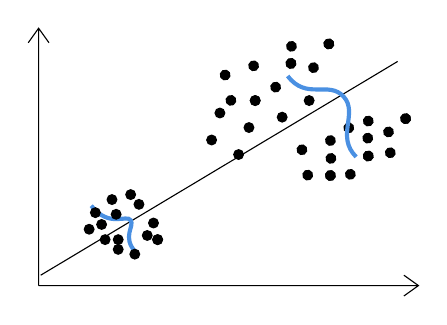
\begin{tikzpicture}[x=0.75pt,y=0.75pt,yscale=-1,xscale=1]
%uncomment if require: \path (0,172.5999984741211); %set diagram left start at 0, and has height of 172.5999984741211

%Straight Lines [id:da8266924204963051] 
\draw    (63.5,156.6) -- (235.5,53.6) ;


%Curve Lines [id:da017249143283004198] 
\draw [color={rgb, 255:red, 74; green, 144; blue, 226 }  ,draw opacity=1 ][line width=1.5]    (87.85,123.1) .. controls (96.5,134) and (104.85,127.1) .. (106.85,130.1) .. controls (108.85,133.1) and (102.5,138) .. (109.2,145.45) ;


%Shape: Axis 2D [id:dp6500078111982048] 
\draw  (62.5,161.6) -- (245.5,161.6)(62.5,37.6) -- (62.5,161.6) -- cycle (238.5,156.6) -- (245.5,161.6) -- (238.5,166.6) (57.5,44.6) -- (62.5,37.6) -- (67.5,44.6)  ;
%Shape: Circle [id:dp27050926560484734] 
\draw  [fill={rgb, 255:red, 0; green, 0; blue, 0 }  ,fill opacity=1 ] (190.5,72.45) .. controls (190.5,71.15) and (191.55,70.1) .. (192.85,70.1) .. controls (194.15,70.1) and (195.2,71.15) .. (195.2,72.45) .. controls (195.2,73.75) and (194.15,74.8) .. (192.85,74.8) .. controls (191.55,74.8) and (190.5,73.75) .. (190.5,72.45) -- cycle ;
%Shape: Circle [id:dp7115090045976589] 
\draw  [fill={rgb, 255:red, 0; green, 0; blue, 0 }  ,fill opacity=1 ] (219.06,98.53) .. controls (219.42,97.28) and (220.71,96.55) .. (221.96,96.91) .. controls (223.21,97.26) and (223.94,98.56) .. (223.59,99.81) .. controls (223.23,101.06) and (221.93,101.78) .. (220.68,101.43) .. controls (219.44,101.08) and (218.71,99.78) .. (219.06,98.53) -- cycle ;
%Shape: Circle [id:dp8518252565776117] 
\draw  [fill={rgb, 255:red, 0; green, 0; blue, 0 }  ,fill opacity=1 ] (219.06,98.53) .. controls (219.42,97.28) and (220.71,96.55) .. (221.96,96.91) .. controls (223.21,97.26) and (223.94,98.56) .. (223.59,99.81) .. controls (223.23,101.06) and (221.93,101.78) .. (220.68,101.43) .. controls (219.44,101.08) and (218.71,99.78) .. (219.06,98.53) -- cycle ;
%Shape: Circle [id:dp9888308723757226] 
\draw  [fill={rgb, 255:red, 0; green, 0; blue, 0 }  ,fill opacity=1 ] (177.5,80.45) .. controls (177.5,79.15) and (178.55,78.1) .. (179.85,78.1) .. controls (181.15,78.1) and (182.2,79.15) .. (182.2,80.45) .. controls (182.2,81.75) and (181.15,82.8) .. (179.85,82.8) .. controls (178.55,82.8) and (177.5,81.75) .. (177.5,80.45) -- cycle ;
%Shape: Circle [id:dp7697187523470395] 
\draw  [fill={rgb, 255:red, 0; green, 0; blue, 0 }  ,fill opacity=1 ] (201.07,99.68) .. controls (201.42,98.43) and (202.72,97.7) .. (203.97,98.06) .. controls (205.22,98.41) and (205.95,99.71) .. (205.59,100.96) .. controls (205.24,102.21) and (203.94,102.93) .. (202.69,102.58) .. controls (201.44,102.23) and (200.72,100.93) .. (201.07,99.68) -- cycle ;
%Shape: Circle [id:dp6429205670686] 
\draw  [fill={rgb, 255:red, 0; green, 0; blue, 0 }  ,fill opacity=1 ] (209.68,84.95) .. controls (210.03,83.7) and (211.33,82.98) .. (212.58,83.33) .. controls (213.83,83.68) and (214.55,84.98) .. (214.2,86.23) .. controls (213.85,87.48) and (212.55,88.2) .. (211.3,87.85) .. controls (210.05,87.5) and (209.32,86.2) .. (209.68,84.95) -- cycle ;
%Shape: Circle [id:dp18324700717368003] 
\draw  [fill={rgb, 255:red, 0; green, 0; blue, 0 }  ,fill opacity=1 ] (200.82,107.92) .. controls (201.17,106.67) and (202.47,105.95) .. (203.72,106.3) .. controls (204.97,106.65) and (205.7,107.95) .. (205.34,109.2) .. controls (204.99,110.45) and (203.69,111.18) .. (202.44,110.82) .. controls (201.19,110.47) and (200.47,109.17) .. (200.82,107.92) -- cycle ;
%Shape: Circle [id:dp404835811750923] 
\draw  [fill={rgb, 255:red, 0; green, 0; blue, 0 }  ,fill opacity=1 ] (200.82,107.92) .. controls (201.17,106.67) and (202.47,105.95) .. (203.72,106.3) .. controls (204.97,106.65) and (205.7,107.95) .. (205.34,109.2) .. controls (204.99,110.45) and (203.69,111.18) .. (202.44,110.82) .. controls (201.19,110.47) and (200.47,109.17) .. (200.82,107.92) -- cycle ;
%Shape: Circle [id:dp5057643743008591] 
\draw  [fill={rgb, 255:red, 0; green, 0; blue, 0 }  ,fill opacity=1 ] (164.5,72.45) .. controls (164.5,71.15) and (165.55,70.1) .. (166.85,70.1) .. controls (168.15,70.1) and (169.2,71.15) .. (169.2,72.45) .. controls (169.2,73.75) and (168.15,74.8) .. (166.85,74.8) .. controls (165.55,74.8) and (164.5,73.75) .. (164.5,72.45) -- cycle ;
%Shape: Circle [id:dp0340921138911765] 
\draw  [fill={rgb, 255:red, 0; green, 0; blue, 0 }  ,fill opacity=1 ] (164.5,72.45) .. controls (164.5,71.15) and (165.55,70.1) .. (166.85,70.1) .. controls (168.15,70.1) and (169.2,71.15) .. (169.2,72.45) .. controls (169.2,73.75) and (168.15,74.8) .. (166.85,74.8) .. controls (165.55,74.8) and (164.5,73.75) .. (164.5,72.45) -- cycle ;
%Shape: Circle [id:dp9411008922183792] 
\draw  [fill={rgb, 255:red, 0; green, 0; blue, 0 }  ,fill opacity=1 ] (147.5,78.45) .. controls (147.5,77.15) and (148.55,76.1) .. (149.85,76.1) .. controls (151.15,76.1) and (152.2,77.15) .. (152.2,78.45) .. controls (152.2,79.75) and (151.15,80.8) .. (149.85,80.8) .. controls (148.55,80.8) and (147.5,79.75) .. (147.5,78.45) -- cycle ;
%Shape: Circle [id:dp216792083895468] 
\draw  [fill={rgb, 255:red, 0; green, 0; blue, 0 }  ,fill opacity=1 ] (161.5,85.45) .. controls (161.5,84.15) and (162.55,83.1) .. (163.85,83.1) .. controls (165.15,83.1) and (166.2,84.15) .. (166.2,85.45) .. controls (166.2,86.75) and (165.15,87.8) .. (163.85,87.8) .. controls (162.55,87.8) and (161.5,86.75) .. (161.5,85.45) -- cycle ;
%Shape: Circle [id:dp2819365889401646] 
\draw  [fill={rgb, 255:red, 0; green, 0; blue, 0 }  ,fill opacity=1 ] (143.5,91.45) .. controls (143.5,90.15) and (144.55,89.1) .. (145.85,89.1) .. controls (147.15,89.1) and (148.2,90.15) .. (148.2,91.45) .. controls (148.2,92.75) and (147.15,93.8) .. (145.85,93.8) .. controls (144.55,93.8) and (143.5,92.75) .. (143.5,91.45) -- cycle ;
%Shape: Circle [id:dp11509146456450803] 
\draw  [fill={rgb, 255:red, 0; green, 0; blue, 0 }  ,fill opacity=1 ] (156.5,98.45) .. controls (156.5,97.15) and (157.55,96.1) .. (158.85,96.1) .. controls (160.15,96.1) and (161.2,97.15) .. (161.2,98.45) .. controls (161.2,99.75) and (160.15,100.8) .. (158.85,100.8) .. controls (157.55,100.8) and (156.5,99.75) .. (156.5,98.45) -- cycle ;
%Shape: Circle [id:dp3532763929660385] 
\draw  [fill={rgb, 255:red, 0; green, 0; blue, 0 }  ,fill opacity=1 ] (90.5,132.15) .. controls (90.5,130.85) and (91.55,129.8) .. (92.85,129.8) .. controls (94.15,129.8) and (95.2,130.85) .. (95.2,132.15) .. controls (95.2,133.45) and (94.15,134.5) .. (92.85,134.5) .. controls (91.55,134.5) and (90.5,133.45) .. (90.5,132.15) -- cycle ;
%Shape: Circle [id:dp9366915298169731] 
\draw  [fill={rgb, 255:red, 0; green, 0; blue, 0 }  ,fill opacity=1 ] (92.2,139.45) .. controls (92.2,138.15) and (93.25,137.1) .. (94.55,137.1) .. controls (95.85,137.1) and (96.9,138.15) .. (96.9,139.45) .. controls (96.9,140.75) and (95.85,141.8) .. (94.55,141.8) .. controls (93.25,141.8) and (92.2,140.75) .. (92.2,139.45) -- cycle ;
%Shape: Circle [id:dp5553925314838524] 
\draw  [fill={rgb, 255:red, 0; green, 0; blue, 0 }  ,fill opacity=1 ] (98.5,144.15) .. controls (98.5,142.85) and (99.55,141.8) .. (100.85,141.8) .. controls (102.15,141.8) and (103.2,142.85) .. (103.2,144.15) .. controls (103.2,145.45) and (102.15,146.5) .. (100.85,146.5) .. controls (99.55,146.5) and (98.5,145.45) .. (98.5,144.15) -- cycle ;
%Shape: Circle [id:dp39470422497531876] 
\draw  [fill={rgb, 255:red, 0; green, 0; blue, 0 }  ,fill opacity=1 ] (108.5,122.45) .. controls (108.5,121.15) and (109.55,120.1) .. (110.85,120.1) .. controls (112.15,120.1) and (113.2,121.15) .. (113.2,122.45) .. controls (113.2,123.75) and (112.15,124.8) .. (110.85,124.8) .. controls (109.55,124.8) and (108.5,123.75) .. (108.5,122.45) -- cycle ;
%Shape: Circle [id:dp8929280115771256] 
\draw  [fill={rgb, 255:red, 0; green, 0; blue, 0 }  ,fill opacity=1 ] (115.5,131.45) .. controls (115.5,130.15) and (116.55,129.1) .. (117.85,129.1) .. controls (119.15,129.1) and (120.2,130.15) .. (120.2,131.45) .. controls (120.2,132.75) and (119.15,133.8) .. (117.85,133.8) .. controls (116.55,133.8) and (115.5,132.75) .. (115.5,131.45) -- cycle ;
%Shape: Circle [id:dp5697394685258441] 
\draw  [fill={rgb, 255:red, 0; green, 0; blue, 0 }  ,fill opacity=1 ] (112.5,137.45) .. controls (112.5,136.15) and (113.55,135.1) .. (114.85,135.1) .. controls (116.15,135.1) and (117.2,136.15) .. (117.2,137.45) .. controls (117.2,138.75) and (116.15,139.8) .. (114.85,139.8) .. controls (113.55,139.8) and (112.5,138.75) .. (112.5,137.45) -- cycle ;
%Shape: Circle [id:dp1478989499447756] 
\draw  [fill={rgb, 255:red, 0; green, 0; blue, 0 }  ,fill opacity=1 ] (117.5,139.45) .. controls (117.5,138.15) and (118.55,137.1) .. (119.85,137.1) .. controls (121.15,137.1) and (122.2,138.15) .. (122.2,139.45) .. controls (122.2,140.75) and (121.15,141.8) .. (119.85,141.8) .. controls (118.55,141.8) and (117.5,140.75) .. (117.5,139.45) -- cycle ;
%Shape: Circle [id:dp654616365009905] 
\draw  [fill={rgb, 255:red, 0; green, 0; blue, 0 }  ,fill opacity=1 ] (117.5,139.45) .. controls (117.5,138.15) and (118.55,137.1) .. (119.85,137.1) .. controls (121.15,137.1) and (122.2,138.15) .. (122.2,139.45) .. controls (122.2,140.75) and (121.15,141.8) .. (119.85,141.8) .. controls (118.55,141.8) and (117.5,140.75) .. (117.5,139.45) -- cycle ;
%Shape: Circle [id:dp38092850325576166] 
\draw  [fill={rgb, 255:red, 0; green, 0; blue, 0 }  ,fill opacity=1 ] (106.5,146.45) .. controls (106.5,145.15) and (107.55,144.1) .. (108.85,144.1) .. controls (110.15,144.1) and (111.2,145.15) .. (111.2,146.45) .. controls (111.2,147.75) and (110.15,148.8) .. (108.85,148.8) .. controls (107.55,148.8) and (106.5,147.75) .. (106.5,146.45) -- cycle ;
%Shape: Circle [id:dp6590284624362692] 
\draw  [fill={rgb, 255:red, 0; green, 0; blue, 0 }  ,fill opacity=1 ] (104.5,117.75) .. controls (104.5,116.45) and (105.55,115.4) .. (106.85,115.4) .. controls (108.15,115.4) and (109.2,116.45) .. (109.2,117.75) .. controls (109.2,119.05) and (108.15,120.1) .. (106.85,120.1) .. controls (105.55,120.1) and (104.5,119.05) .. (104.5,117.75) -- cycle ;
%Shape: Circle [id:dp326489394414073] 
\draw  [fill={rgb, 255:red, 0; green, 0; blue, 0 }  ,fill opacity=1 ] (95.5,120.15) .. controls (95.5,118.85) and (96.55,117.8) .. (97.85,117.8) .. controls (99.15,117.8) and (100.2,118.85) .. (100.2,120.15) .. controls (100.2,121.45) and (99.15,122.5) .. (97.85,122.5) .. controls (96.55,122.5) and (95.5,121.45) .. (95.5,120.15) -- cycle ;
%Shape: Circle [id:dp617063968905118] 
\draw  [fill={rgb, 255:red, 0; green, 0; blue, 0 }  ,fill opacity=1 ] (97.5,127.25) .. controls (97.5,125.95) and (98.55,124.9) .. (99.85,124.9) .. controls (101.15,124.9) and (102.2,125.95) .. (102.2,127.25) .. controls (102.2,128.55) and (101.15,129.6) .. (99.85,129.6) .. controls (98.55,129.6) and (97.5,128.55) .. (97.5,127.25) -- cycle ;
%Shape: Circle [id:dp5631657085776833] 
\draw  [fill={rgb, 255:red, 0; green, 0; blue, 0 }  ,fill opacity=1 ] (87.5,126.45) .. controls (87.5,125.15) and (88.55,124.1) .. (89.85,124.1) .. controls (91.15,124.1) and (92.2,125.15) .. (92.2,126.45) .. controls (92.2,127.75) and (91.15,128.8) .. (89.85,128.8) .. controls (88.55,128.8) and (87.5,127.75) .. (87.5,126.45) -- cycle ;
%Shape: Circle [id:dp07505235674911326] 
\draw  [fill={rgb, 255:red, 0; green, 0; blue, 0 }  ,fill opacity=1 ] (98.5,139.45) .. controls (98.5,138.15) and (99.55,137.1) .. (100.85,137.1) .. controls (102.15,137.1) and (103.2,138.15) .. (103.2,139.45) .. controls (103.2,140.75) and (102.15,141.8) .. (100.85,141.8) .. controls (99.55,141.8) and (98.5,140.75) .. (98.5,139.45) -- cycle ;
%Shape: Circle [id:dp2914438352074973] 
\draw  [fill={rgb, 255:red, 0; green, 0; blue, 0 }  ,fill opacity=1 ] (84.5,134.45) .. controls (84.5,133.15) and (85.55,132.1) .. (86.85,132.1) .. controls (88.15,132.1) and (89.2,133.15) .. (89.2,134.45) .. controls (89.2,135.75) and (88.15,136.8) .. (86.85,136.8) .. controls (85.55,136.8) and (84.5,135.75) .. (84.5,134.45) -- cycle ;
%Curve Lines [id:da6091015187110322] 
\draw [color={rgb, 255:red, 74; green, 144; blue, 226 }  ,draw opacity=1 ][line width=1.5]    (182.5,60.6) .. controls (191.5,72.6) and (202.33,62.6) .. (209.5,70.6) .. controls (216.67,78.6) and (205.5,89.6) .. (215.5,99.6) ;


%Shape: Circle [id:dp6278328411998773] 
\draw  [fill={rgb, 255:red, 0; green, 0; blue, 0 }  ,fill opacity=1 ] (237.06,80.53) .. controls (237.42,79.28) and (238.71,78.55) .. (239.96,78.91) .. controls (241.21,79.26) and (241.94,80.56) .. (241.59,81.81) .. controls (241.23,83.06) and (239.93,83.78) .. (238.68,83.43) .. controls (237.44,83.08) and (236.71,81.78) .. (237.06,80.53) -- cycle ;
%Shape: Circle [id:dp2651029250538355] 
\draw  [fill={rgb, 255:red, 0; green, 0; blue, 0 }  ,fill opacity=1 ] (237.06,80.53) .. controls (237.42,79.28) and (238.71,78.55) .. (239.96,78.91) .. controls (241.21,79.26) and (241.94,80.56) .. (241.59,81.81) .. controls (241.23,83.06) and (239.93,83.78) .. (238.68,83.43) .. controls (237.44,83.08) and (236.71,81.78) .. (237.06,80.53) -- cycle ;
%Shape: Circle [id:dp10116171581038036] 
\draw  [fill={rgb, 255:red, 0; green, 0; blue, 0 }  ,fill opacity=1 ] (219.07,81.68) .. controls (219.42,80.43) and (220.72,79.7) .. (221.97,80.06) .. controls (223.22,80.41) and (223.95,81.71) .. (223.59,82.96) .. controls (223.24,84.21) and (221.94,84.93) .. (220.69,84.58) .. controls (219.44,84.23) and (218.72,82.93) .. (219.07,81.68) -- cycle ;
%Shape: Circle [id:dp14302796062319412] 
\draw  [fill={rgb, 255:red, 0; green, 0; blue, 0 }  ,fill opacity=1 ] (229.68,96.95) .. controls (230.03,95.7) and (231.33,94.98) .. (232.58,95.33) .. controls (233.83,95.68) and (234.55,96.98) .. (234.2,98.23) .. controls (233.85,99.48) and (232.55,100.2) .. (231.3,99.85) .. controls (230.05,99.5) and (229.32,98.2) .. (229.68,96.95) -- cycle ;
%Shape: Circle [id:dp3390139842836206] 
\draw  [fill={rgb, 255:red, 0; green, 0; blue, 0 }  ,fill opacity=1 ] (218.82,89.92) .. controls (219.17,88.67) and (220.47,87.95) .. (221.72,88.3) .. controls (222.97,88.65) and (223.7,89.95) .. (223.34,91.2) .. controls (222.99,92.45) and (221.69,93.18) .. (220.44,92.82) .. controls (219.19,92.47) and (218.47,91.17) .. (218.82,89.92) -- cycle ;
%Shape: Circle [id:dp5779580928534842] 
\draw  [fill={rgb, 255:red, 0; green, 0; blue, 0 }  ,fill opacity=1 ] (228.82,86.92) .. controls (229.17,85.67) and (230.47,84.95) .. (231.72,85.3) .. controls (232.97,85.65) and (233.7,86.95) .. (233.34,88.2) .. controls (232.99,89.45) and (231.69,90.18) .. (230.44,89.82) .. controls (229.19,89.47) and (228.47,88.17) .. (228.82,86.92) -- cycle ;
%Shape: Circle [id:dp8926721968361584] 
\draw  [fill={rgb, 255:red, 0; green, 0; blue, 0 }  ,fill opacity=1 ] (200.83,91.07) .. controls (201.18,89.82) and (202.48,89.1) .. (203.73,89.45) .. controls (204.98,89.8) and (205.71,91.1) .. (205.35,92.35) .. controls (205,93.6) and (203.7,94.33) .. (202.45,93.97) .. controls (201.2,93.62) and (200.48,92.32) .. (200.83,91.07) -- cycle ;
%Shape: Circle [id:dp3658495148907712] 
\draw  [fill={rgb, 255:red, 0; green, 0; blue, 0 }  ,fill opacity=1 ] (210.44,107.34) .. controls (210.79,106.1) and (212.09,105.37) .. (213.34,105.72) .. controls (214.59,106.07) and (215.31,107.37) .. (214.96,108.62) .. controls (214.61,109.87) and (213.31,110.6) .. (212.06,110.24) .. controls (210.81,109.89) and (210.08,108.59) .. (210.44,107.34) -- cycle ;
%Shape: Circle [id:dp984762104794698] 
\draw  [fill={rgb, 255:red, 0; green, 0; blue, 0 }  ,fill opacity=1 ] (189.89,107.72) .. controls (190.24,106.48) and (191.54,105.75) .. (192.79,106.1) .. controls (194.04,106.46) and (194.76,107.75) .. (194.41,109) .. controls (194.06,110.25) and (192.76,110.98) .. (191.51,110.63) .. controls (190.26,110.27) and (189.54,108.97) .. (189.89,107.72) -- cycle ;
%Shape: Circle [id:dp4998558602671004] 
\draw  [fill={rgb, 255:red, 0; green, 0; blue, 0 }  ,fill opacity=1 ] (187.11,95.51) .. controls (187.46,94.26) and (188.76,93.53) .. (190.01,93.89) .. controls (191.26,94.24) and (191.98,95.54) .. (191.63,96.79) .. controls (191.28,98.03) and (189.98,98.76) .. (188.73,98.41) .. controls (187.48,98.06) and (186.75,96.76) .. (187.11,95.51) -- cycle ;
%Shape: Circle [id:dp681828512542674] 
\draw  [fill={rgb, 255:red, 0; green, 0; blue, 0 }  ,fill opacity=1 ] (200.06,44.53) .. controls (200.42,43.28) and (201.71,42.55) .. (202.96,42.91) .. controls (204.21,43.26) and (204.94,44.56) .. (204.59,45.81) .. controls (204.23,47.06) and (202.93,47.78) .. (201.68,47.43) .. controls (200.44,47.08) and (199.71,45.78) .. (200.06,44.53) -- cycle ;
%Shape: Circle [id:dp17259944260891236] 
\draw  [fill={rgb, 255:red, 0; green, 0; blue, 0 }  ,fill opacity=1 ] (200.06,44.53) .. controls (200.42,43.28) and (201.71,42.55) .. (202.96,42.91) .. controls (204.21,43.26) and (204.94,44.56) .. (204.59,45.81) .. controls (204.23,47.06) and (202.93,47.78) .. (201.68,47.43) .. controls (200.44,47.08) and (199.71,45.78) .. (200.06,44.53) -- cycle ;
%Shape: Circle [id:dp7893747429900331] 
\draw  [fill={rgb, 255:red, 0; green, 0; blue, 0 }  ,fill opacity=1 ] (182.07,45.68) .. controls (182.42,44.43) and (183.72,43.7) .. (184.97,44.06) .. controls (186.22,44.41) and (186.95,45.71) .. (186.59,46.96) .. controls (186.24,48.21) and (184.94,48.93) .. (183.69,48.58) .. controls (182.44,48.23) and (181.72,46.93) .. (182.07,45.68) -- cycle ;
%Shape: Circle [id:dp8699303385493997] 
\draw  [fill={rgb, 255:red, 0; green, 0; blue, 0 }  ,fill opacity=1 ] (192.68,55.95) .. controls (193.03,54.7) and (194.33,53.98) .. (195.58,54.33) .. controls (196.83,54.68) and (197.55,55.98) .. (197.2,57.23) .. controls (196.85,58.48) and (195.55,59.2) .. (194.3,58.85) .. controls (193.05,58.5) and (192.32,57.2) .. (192.68,55.95) -- cycle ;
%Shape: Circle [id:dp2647855008094744] 
\draw  [fill={rgb, 255:red, 0; green, 0; blue, 0 }  ,fill opacity=1 ] (181.82,53.92) .. controls (182.17,52.67) and (183.47,51.95) .. (184.72,52.3) .. controls (185.97,52.65) and (186.7,53.95) .. (186.34,55.2) .. controls (185.99,56.45) and (184.69,57.18) .. (183.44,56.82) .. controls (182.19,56.47) and (181.47,55.17) .. (181.82,53.92) -- cycle ;
%Shape: Circle [id:dp1537547978351581] 
\draw  [fill={rgb, 255:red, 0; green, 0; blue, 0 }  ,fill opacity=1 ] (181.82,53.92) .. controls (182.17,52.67) and (183.47,51.95) .. (184.72,52.3) .. controls (185.97,52.65) and (186.7,53.95) .. (186.34,55.2) .. controls (185.99,56.45) and (184.69,57.18) .. (183.44,56.82) .. controls (182.19,56.47) and (181.47,55.17) .. (181.82,53.92) -- cycle ;
%Shape: Circle [id:dp14730623417094235] 
\draw  [fill={rgb, 255:red, 0; green, 0; blue, 0 }  ,fill opacity=1 ] (163.83,55.07) .. controls (164.18,53.82) and (165.48,53.1) .. (166.73,53.45) .. controls (167.98,53.8) and (168.71,55.1) .. (168.35,56.35) .. controls (168,57.6) and (166.7,58.33) .. (165.45,57.97) .. controls (164.2,57.62) and (163.48,56.32) .. (163.83,55.07) -- cycle ;
%Shape: Circle [id:dp3428895870133042] 
\draw  [fill={rgb, 255:red, 0; green, 0; blue, 0 }  ,fill opacity=1 ] (174.44,65.34) .. controls (174.79,64.1) and (176.09,63.37) .. (177.34,63.72) .. controls (178.59,64.07) and (179.31,65.37) .. (178.96,66.62) .. controls (178.61,67.87) and (177.31,68.6) .. (176.06,68.24) .. controls (174.81,67.89) and (174.08,66.59) .. (174.44,65.34) -- cycle ;
%Shape: Circle [id:dp6866245110084515] 
\draw  [fill={rgb, 255:red, 0; green, 0; blue, 0 }  ,fill opacity=1 ] (152.89,71.72) .. controls (153.24,70.48) and (154.54,69.75) .. (155.79,70.1) .. controls (157.04,70.46) and (157.76,71.75) .. (157.41,73) .. controls (157.06,74.25) and (155.76,74.98) .. (154.51,74.63) .. controls (153.26,74.27) and (152.54,72.97) .. (152.89,71.72) -- cycle ;
%Shape: Circle [id:dp6203649522817893] 
\draw  [fill={rgb, 255:red, 0; green, 0; blue, 0 }  ,fill opacity=1 ] (150.11,59.51) .. controls (150.46,58.26) and (151.76,57.53) .. (153.01,57.89) .. controls (154.26,58.24) and (154.98,59.54) .. (154.63,60.79) .. controls (154.28,62.03) and (152.98,62.76) .. (151.73,62.41) .. controls (150.48,62.06) and (149.75,60.76) .. (150.11,59.51) -- cycle ;

\end{tikzpicture}


On utilise la méthode du \textbf{moindre carré pondéré} (MCP) pour trouver $\widehat{\bm{\beta}}$ tel que:
\[
	\sum_{i = 1}^{n} \omega_{i}(Y_{i} - \widehat{Y}_i)^{2} \Leftrightarrow \widehat{\bm{\epsilon}}^{\top} \matr{V}^{-1} \widehat{\bm{\epsilon}}
	\]
est minimale et qu'on pose :
\begin{align*}
\omega_{i} &\propto 1/\sigma^{2}_{i} \\
\matr{V} &= \text{diag}(\sigma_{1}^{2}, \dots, \sigma_{n}^{2})
\end{align*}
On obtient alors:
\begin{align*}
	\widehat{\bm{\beta}} &= \matr{(X^{\top}V^{-1}X)^{-1}X^{\top}V^{-1}Y} \\
	\text{V}(\widehat{\bm{\beta}}) &= \matr{(X^{\top}V^{-1}X)^{-1}}
\end{align*}
\\
On peut faire le \textbf{test} $H_0 : \beta_j = \beta_{j, 0}$ avec la statistique:
\begin{align*}
	t &= \frac{\widehat{\beta}_{j} - \beta_{j, 0}}{\sqrt{(\matr{X^{\top}V^{-1}X)^{-1}_{jj}}}}
\end{align*}
Et utiliser $V = V^{*}\sigma^{2}$ en estimant $\sigma^{2}$ par:
\begin{align*}
	s^{2} &= \frac{\sum_{i = 1}^{n} \omega_{i}(Y_{i} - \widehat{Y}_i)^{2}}{n - p'}
\end{align*}
\\
On peut contruire une table d'\textbf{analyse de la variance} avec la décomposition:
\begin{align*}
	\underset{SST_V}{\underbrace{\matr{Y^{\top}V^{-1}Y}}} &= \underset{SSR_V}{\underbrace{\bm{\widehat{\beta}} \ \matr{X^{\top}V^{-1}Y}}} + \underset{SSE_V}{\underbrace{(\matr{Y - X}\bm{\widehat{\beta}})^{\top}\matr{V^{-1}}(\matr{Y - X}\bm{\widehat{\beta}}) }}
\end{align*}

\section{Sélection de modèle et régression régularisée}
En présence de beaucoup de variable exogènes, on court le danger d'en garder trop ou pas assez
\begin{itemize}
	\item \textbf{Trop}: On augmente inutilement la variance des estimations $(\hat{\beta})$.
	\item \textbf{Moins}: On simplifie notre modèle trops en augmentant inutilement le biais des estimations $(\hat{\beta})$.
\end{itemize}

\textbf{ajouter information sur début du chapitre pour l'examen}

\subsection*{Critères de comparaison classiques}
\begin{itemize}
	\item Coefficient de détermination (pour mesurer la qualité globale du modèle) :
	\[ R^2 = \frac{SSR}{SST} \]
	Si on ajoute une variable exogène, il est certain que $R^2$ augmentera, on utilise donc ce critère pour valider si la régression est utile pour prédire $Y$, mais pas pour critère de sélection des variables exogènes.
	\item \textbf{Coeficient de détermination ajusté}:
	\[ R_a^2 = \frac{SSE / p}{SST / (n-1)} = \frac{MSE}{MST} \]
	Ce critère permet de valider l'ajout de nouvelles variables exogènes.\\ 
	De plus, \textbf{il peut diminuer avec l'ajout de nouvelles variables}.
\end{itemize}
Ces deux critères sont inutiles pour comparer des modèles avec des transformations différentes et pour des modèles avec/sans ordonnée à l'origine.

\subsection*{Méthode basées sur la puissance de prévision}
Ce critère maximise l'habileté du modèle a prédire de nouvelles données.

\subsubsection*{\textcolor{darkgreen}{Principe de la validation croisée}}
%\subsubsection*{Principe de la validation croisée}

\begin{algo}{Algorithme de validation croisée classique}
\begin{enumerate}
\item Pour $i = 1, ..., n$,
\begin{enumerate}[label=1.\arabic*]
	\item Enlever la $i$\up{e} observation du jeu de données.
	\item Estimer les paramètres du modèle à partir des $n - 1$ données restante.
	\item Prédire $Y_i$ à partir de $x_i$ et du modèle obtenu en 2, noté $\hat{Y}_{i,-i}$
\end{enumerate}
\item Calculer la somme des carrés des erreurs de prévision $PRESS = \sum_{i=1}^n (Y_i - \hat{Y}_{i,-i})^2$
\end{enumerate}
\end{algo}
	On cherche a minimiser le \textbf{PRESS} ou, à maximiser le \textbf{coefficient de détermination de prévision}:
	\[ R_p^2 = 1 - \frac{PRESS}{SST} = 1 - \frac{\sum_{i=1}^n (Y_i - \hat{Y}_{i,-i})^2}{\sum_{i=1}^n (Y_i - \bar{Y})^2}\]
\subsubsection*{\textcolor{darkgreen}{Les résidus PRESS}}
%\subsubsection*{Les résidus PRESS}
Il est possible de trouver la statistique PRESS sans devoir calculer $n$ régressions :
	\[ PRESS = \sum_{i=1}^n \left( \frac{\hat{\varepsilon}_i}{1 - h_{ii}} \right)^2 \]
	Le i$^{\text{ème}}$ résidu PRESS est le i$^{\text{ème}}$ terme de la sommation. 
	\[
	\widehat{\varepsilon}_{i, -i} = \frac{\widehat{\varepsilon}_{i}}{1 - h_{ii}}
	\]	
Utile dans le cas où il n'aurait qu'un seul résidu mauvais qui biaise la sommation.

\subsubsection*{\textcolor{darkgreen}{Échantillion de test et validation croisée par $k$ ensemble}}
%\subsubsection*{Échantillion de test et validation croisée par $k$ ensemble}
Le \textbf{dernier recourt} après avoir essayé tous les autres tests.\\
Lorsqu'on a un très grand jeu de données, on peut les séparer en deux: 
\begin{description}
	\item[\textbf{Training set}]: Utilisé pour ajuster le modèle et faire la sélection de variables explicatives.
	\item[\textbf{Test set}]: Échantillon sur lequel on effectue des prévisions.
\end{description}
La puissance de prévision est donc calculé avec:
\begin{align*}
	\text{\textbf{MSEP}} &= \frac{1}{n_{\text{test}}} \sum_{i \in \text{test}} (Y_{i} - \widehat{Y}_{i})^{2}
\end{align*}

\begin{algo}{Algorithme de validation croisée par K ensembles}
\begin{enumerate}
\item Pour $k = 1, ..., K$,
\begin{enumerate}[label=1.\arabic*]
	\item Enlever le $k$\up{e} ensemble du jeu de donnée.
	\item  Estimer les paramètres du modèle à partir des données des $k - 1$ échantillons restants.
	\item Prédire les observations du $k$\up{e} ensemble $(\hat{Y}_{i,-k})$ et calculer
	\[ MSEP_k = \frac{1}{n_k} \sum_{i\in group\:k} (Y_i - \hat{Y}_{i,-k})^2 \]
\end{enumerate}
	\item Calculer la moyenne des sommes des carrés des erreurs de prévision $\frac{1}{k} \sum_{k=1}^k MSEP_k$
\end{enumerate}
	On choisit le modèle qui minimise $\frac{1}{k} \sum_{k=1}^k MSEP_k$
\end{algo}

\subsection*{Le $C_p$ de Mallows}
\begin{align*}
C_p &= p' + \frac{(s_p^2 - \widehat{\sigma}^2)(n - p')}{\widehat{\sigma}^2} \\
&= \frac{SSE}{\widehat{\sigma}^2} + 2p' - n
\end{align*}
On cherche le modèle pour lequel $C_p \approx p'$

\subsection*{Critère d'information d'akaike et critère bayésien de Schwarz}
\begin{itemize}
\item Ce critère est le plus utilisé dans la pratique et permet d'évaluer la qualité de l'ajustement d'un modèle. 
\[ AIC = n \cdot \ln \left(\frac{SSE}{n}\right) + 2p' \]
AIC prend en compte à la fois la qualité des prédictions du modèle et sa complexité.
\item BIC est similaire a AIC, mais la pénalité des paramètres dépend de la taille de l'échantillon.
\[ BIC = n \cdot \ln \left(\frac{SSE}{n}\right) + \ln(n)p' \]
\item On cherche donc à minimiser ces 2 critères.
\end{itemize}

\subsection*{Méthode algorithmiques}

%\subsubsection*{Méthode d'inclusion (\textit{forward})}
\begin{enumerate}
\begin{algo}{Méthode d'inclusion forward}
\item On commence avec le modèle le plus simple (i.e. $\hat{Y}_i = \beta_0$)
\item On essaie d'ajouter la variable qui, en l'incluant dans le modèle, permet de réduire le plus le $SSE$ du modèle.
\item On valide si la variable diminue de façon significative les résidus avec un test $F$, où
\begin{align*}
F_{obs} = \frac{SSE_{\text{petit modèle}} - SSE_{\text{grand modèle}}}{SSE_{\text{grand modèle}} / (n-p')}
\end{align*}
On ajoute la variable au modèle si
\begin{align*}
F_{obs} > F_{1, n-p'}(1 - \alpha)
\end{align*}
\item On répète jusqu'à ce qu'aucune variable ne vaille la peine d'être ajoutée.
\end{algo}
\end{enumerate}

%\subsubsection*{Méthode d'exclusion (\textit{backward})}
\begin{enumerate}
\begin{algo}{Méthode d'exclusion backward}

\item On débute avec le modèle complet
\item On veut enlever la variable exogène qui, en l'excluant du modèle, permet de minimiser l'augmentation du $SSE$ de la régression.
\item Même test $F$ qu'à l'étape 3 de la méthode \textit{forward}, sauf qu'on enlève la variable seulement si
\begin{align*}
F_{obs} < F_{1, n-p'}(1-\alpha)
\end{align*}
\item On répète jusqu'à ce qu'aucune variable ne vaille la peine d'être enlevée.

\end{algo}
\end{enumerate}

%\subsubsection*{Méthode pas à pas (\textit{step-wise})}
\begin{enumerate}
\begin{algo}{Méthode pas à pas (step-wise)}

\item On débute avec la méthode d'inclusion
\item Après l'ajout d'une variable au modèle, on effectue la méthode d'exclusion pour les variables qui sont actuellement dans le modèle (on remet constamment le modèle en question).
\end{algo}
\end{enumerate}

%
%Critères par ordre dans laquelle les utiliser:
%\begin{enumerate}
%	\item $C_{p}$ de Mallows
%	\item La sélection pas à pas
%	\item La méthode d'exclusion
%	\item La méthode d'inclusion
%	\item $R_{a}^{2}$
%	\item $R^{2}$
%\end{enumerate}

\subsection*{Graphique des variables ajoutées}



\subsection*{Régression Ridge}

Deux normes sont utilisées en régression, les normes L2 \textit{(régression Ridge)} et L1 \textit{(régression Lasso)}. 
\begin{align*}
\norm{\bm{\beta}}_2 &= \sqrt{\sum_{j = 1}^{p} \beta_{j}^{2}} &
\norm{\bm{\beta}}_1 &= \sum_{j = 1}^{p} \left|\beta_{j} \right|
\end{align*}

La \textbf{régression Ridge} est habituellement utilisée lorsque nous avons une variance très élevée avec l'estimateur BLUE.

Souvent, ceci est lorsqu'il y a beaucoup de variables explicatives qui sont \textbf{possiblement corrélés}.

La méthode consiste à minimiser l'estimateur en acceptant un certain biais \textit{(budget total)} $t$.

Donc, à minimiser la variance de l'estimateur sous la contrainte que $\norm{\bm{\beta}}_2 = \sqrt{\sum_{j = 1}^{p} \beta_{j}^{2}} \le t$.

Cette condition représente un cercle dont on prends \textcolor{red}{le point le plus près} de \textcolor{darkpastelpurple}{l'estimateur OLS $\widehat\beta$}; c'est-à-dire, qu'on prends le point qui est \textit{on the "\textbf{\color{red}ridge}" of the circle}.

Les lignes \textcolor{orange}{oranges} représentent différentes valeurs possible que peuvent prendre $\widehat\beta$.s


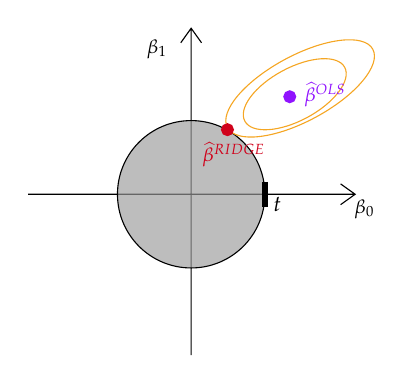
\begin{tikzpicture}[x=0.75pt,y=0.75pt,yscale=-1,xscale=1]
%uncomment if require: \path (0,219.79999923706055); %set diagram left start at 0, and has height of 219.79999923706055

%Shape: Axis 2D [id:dp8001321750733121] 
\draw  (12,82) -- (169.5,82)(90.5,2) -- (90.5,159.5) (162.5,77) -- (169.5,82) -- (162.5,87) (85.5,9) -- (90.5,2) -- (95.5,9)  ;
%Shape: Circle [id:dp06156224627946494] 
\draw  [fill={rgb, 255:red, 155; green, 155; blue, 155 }  ,fill opacity=0.66 ] (55,82) .. controls (55,62.39) and (70.89,46.5) .. (90.5,46.5) .. controls (110.11,46.5) and (126,62.39) .. (126,82) .. controls (126,101.61) and (110.11,117.5) .. (90.5,117.5) .. controls (70.89,117.5) and (55,101.61) .. (55,82) -- cycle ;
%Straight Lines [id:da4393370978295319] 
\draw [line width=2.25]    (126,76) -- (126,88) ;


%Shape: Circle [id:dp07216861586445678] 
\draw  [color={rgb, 255:red, 144; green, 19; blue, 254 }  ,draw opacity=1 ][fill={rgb, 255:red, 144; green, 19; blue, 254 }  ,fill opacity=1 ][line width=3]  (137,35) .. controls (137,34.45) and (137.45,34) .. (138,34) .. controls (138.55,34) and (139,34.45) .. (139,35) .. controls (139,35.55) and (138.55,36) .. (138,36) .. controls (137.45,36) and (137,35.55) .. (137,35) -- cycle ;
%Shape: Ellipse [id:dp9690307834415508] 
\draw  [color={rgb, 255:red, 245; green, 166; blue, 35 }  ,draw opacity=1 ] (116.36,46.77) .. controls (113.03,40.6) and (121.1,29.78) .. (134.39,22.62) .. controls (147.67,15.45) and (161.14,14.65) .. (164.47,20.82) .. controls (167.8,27) and (159.73,37.81) .. (146.45,44.97) .. controls (133.16,52.14) and (119.69,52.94) .. (116.36,46.77) -- cycle ;
%Shape: Ellipse [id:dp42215493996948195] 
\draw  [color={rgb, 255:red, 245; green, 166; blue, 35 }  ,draw opacity=1 ] (107.99,49.88) .. controls (103.85,42.22) and (116.18,27.55) .. (135.51,17.12) .. controls (154.85,6.69) and (173.88,4.45) .. (178.01,12.12) .. controls (182.15,19.78) and (169.82,34.45) .. (150.49,44.88) .. controls (131.15,55.31) and (112.12,57.55) .. (107.99,49.88) -- cycle ;
%Shape: Circle [id:dp9217179943038853] 
\draw  [color={rgb, 255:red, 208; green, 2; blue, 27 }  ,draw opacity=1 ][fill={rgb, 255:red, 208; green, 2; blue, 27 }  ,fill opacity=1 ][line width=3]  (106.99,50.88) .. controls (106.99,50.33) and (107.44,49.88) .. (107.99,49.88) .. controls (108.54,49.88) and (108.99,50.33) .. (108.99,50.88) .. controls (108.99,51.44) and (108.54,51.88) .. (107.99,51.88) .. controls (107.44,51.88) and (106.99,51.44) .. (106.99,50.88) -- cycle ;

% Text Node
\draw (132,87) node [scale=0.8] [align=left] {$\displaystyle t$};
% Text Node
\draw (155,34) node [scale=0.7,color={rgb, 255:red, 144; green, 19; blue, 254 }  ,opacity=1 ]  {$\widehat{\beta}^{OLS}$};
% Text Node
\draw (111,63) node [scale=0.7,color={rgb, 255:red, 208; green, 2; blue, 27 }  ,opacity=1 ]  {$\widehat{\beta}^{RIDGE}$};
% Text Node
\draw (174,89) node [scale=0.7]  {$\beta _{0}$};
% Text Node
\draw (74,12) node [scale=0.7]  {$\beta _{1}$};


\end{tikzpicture}


On veut minimiser l'équation suivante : 
\begin{align*}
S^{R}(\beta) &= \sum_{i=1}^{n} \left( y_i - \beta_0 - \sum_{j=1}^{p} \beta_j x_{ij} \right)^2 + \lambda \sum_{j=1}^{p} \beta_j^2  
\end{align*}
Et on trouve que
\[\hat{\bm{\beta}}^{R} = \left( \matr{X}^\top \matr{X} + \lambda \matr{I}_p \right)^{-1}  \matr{X}^\top \matr{Y}  \]

On choisit la valeur optimale pour le coefficient de régularisation $\lambda$ avec une validation croisée.


\subsection*{Régression Lasso (\emph{Least Absolute Shrinkage and Selection Operator})}

La \textbf{régression Lasso} est habituellement utilisée pour la sélection de variables.

Souvent, notre estimateur va tomber sur un des coins du diamant, ce qui implique qu'un paramètre serait à 0. 

Donc, nous pouvons mettre à 0 des paramètres contrairement à la régression \textbf{Ridge} où les paramètres peuvent être près de 0 mais très rarement égale à 0.

La méthode minimise la variance de l'estimateur sous la contrainte que $\norm{\bm{\beta}}_1 = \sum_{j = 1}^{p} \left|\beta_{j} \right| \le t$.

Cette condition représente le diamant de l'image dont on prends \textcolor{red}{le point le plus près} de \textcolor{darkpastelpurple}{l'estimateur OLS $\widehat\beta$}.  

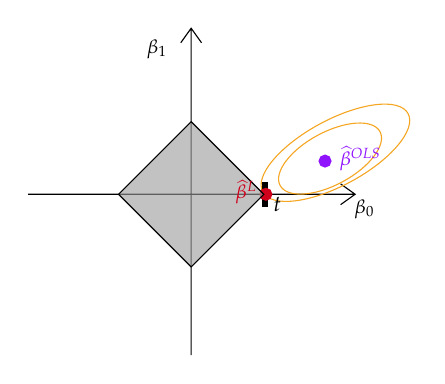
\begin{tikzpicture}[x=0.75pt,y=0.75pt,yscale=-1,xscale=1]
%uncomment if require: \path (0,219.79999923706055); %set diagram left start at 0, and has height of 219.79999923706055

%Shape: Axis 2D [id:dp8001321750733121] 
\draw  (12,82) -- (169.5,82)(90.5,2) -- (90.5,159.5) (162.5,77) -- (169.5,82) -- (162.5,87) (85.5,9) -- (90.5,2) -- (95.5,9)  ;
%Straight Lines [id:da4393370978295319] 
\draw [line width=2.25]    (126,76) -- (126,88) ;


%Shape: Circle [id:dp07216861586445678] 
\draw  [color={rgb, 255:red, 144; green, 19; blue, 254 }  ,draw opacity=1 ][fill={rgb, 255:red, 144; green, 19; blue, 254 }  ,fill opacity=1 ][line width=3]  (154,66) .. controls (154,65.45) and (154.45,65) .. (155,65) .. controls (155.55,65) and (156,65.45) .. (156,66) .. controls (156,66.55) and (155.55,67) .. (155,67) .. controls (154.45,67) and (154,66.55) .. (154,66) -- cycle ;
%Shape: Ellipse [id:dp9690307834415508] 
\draw  [color={rgb, 255:red, 245; green, 166; blue, 35 }  ,draw opacity=1 ] (133.36,77.77) .. controls (130.03,71.6) and (138.1,60.78) .. (151.39,53.62) .. controls (164.67,46.45) and (178.14,45.65) .. (181.47,51.82) .. controls (184.8,58) and (176.73,68.81) .. (163.45,75.97) .. controls (150.16,83.14) and (136.69,83.94) .. (133.36,77.77) -- cycle ;
%Shape: Ellipse [id:dp42215493996948195] 
\draw  [color={rgb, 255:red, 245; green, 166; blue, 35 }  ,draw opacity=1 ] (124.99,80.88) .. controls (120.85,73.22) and (133.18,58.55) .. (152.51,48.12) .. controls (171.85,37.69) and (190.88,35.45) .. (195.01,43.12) .. controls (199.15,50.78) and (186.82,65.45) .. (167.49,75.88) .. controls (148.15,86.31) and (129.12,88.55) .. (124.99,80.88) -- cycle ;
%Shape: Circle [id:dp9217179943038853] 
\draw  [color={rgb, 255:red, 208; green, 2; blue, 27 }  ,draw opacity=1 ][fill={rgb, 255:red, 208; green, 2; blue, 27 }  ,fill opacity=1 ][line width=3]  (125.5,82) .. controls (125.5,81.45) and (125.95,81) .. (126.5,81) .. controls (127.05,81) and (127.5,81.45) .. (127.5,82) .. controls (127.5,82.55) and (127.05,83) .. (126.5,83) .. controls (125.95,83) and (125.5,82.55) .. (125.5,82) -- cycle ;
%Shape: Diamond [id:dp9831296262573708] 
\draw  [fill={rgb, 255:red, 155; green, 155; blue, 155 }  ,fill opacity=0.61 ] (90.5,47) -- (125.5,82) -- (90.5,117) -- (55.5,82) -- cycle ;

% Text Node
\draw (132,87) node [scale=0.8] [align=left] {$\displaystyle t$};
% Text Node
\draw (172,65) node [scale=0.7,color={rgb, 255:red, 144; green, 19; blue, 254 }  ,opacity=1 ]  {$\widehat{\beta}^{OLS}$};
% Text Node
\draw (117,81) node [scale=0.7,color={rgb, 255:red, 208; green, 2; blue, 27 }  ,opacity=1 ]  {$\widehat{\beta}^{L}$};
% Text Node
\draw (174,89) node [scale=0.7]  {$\beta _{0}$};
% Text Node
\draw (74,12) node [scale=0.7]  {$\beta _{1}$};

\end{tikzpicture}


On veut minimiser l'équation suivante:
\begin{align*}
S^{L}(\bm{\beta}) &= 
	\sum_{i=1}^{n} \left( y_i - \beta_0 - \sum_{j=1}^{p} \beta_j x_{ij} \right)^2 
	+ \lambda \sum_{j=1}^{p} | \beta_j | 
\end{align*}

À noter qu'un méthode plus efficace que Ridge et Lasso est de minimiser sous la contrainte que $\sum_{j = 1}^{p} \bm{1}_{\{ \beta_j \neq 0 \}} \le t$.



\section{Modèles linéaires généralisés (GLM)}
\subsection*{Famille exponentielle linéaire}
\subsubsection*{Définition}
Une loi de probabilité fait partie de la famille exponentielle linéaire si
\begin{enumerate}[label=\faAngleRight]
\item On peut exprimer la fonction de densité (ou masse) de probabilité comme
\[f(y ; \theta, \phi) =   \exp \left( \frac{y \theta - b(\theta)}{a(\phi)} + c(y ; \phi)    \right)  \] 
où $\theta$ est le paramètre canonique et $\phi$ est le paramètre de dispersion.

\item la fonction $c$ ne dépend pas du paramètre $\theta$.
\item Le support de $Y$ ne dépend pas des paramètres $\theta$ ou $\phi$.
\end{enumerate}

\subsubsection*{Propriétés}
Soit $\mu = \dot{b}(\theta) = \derivee{\theta} b(\theta)$ et $V(\mu) = \ddot{b}(\theta) = \frac{\partial^2}{\partial \theta^2} b(\theta)$. Alors, si $Y$ fait partie de la famille exponentielle linéaire, on peut exprimer l'espérance et la variance comme
\begin{align*}
\esp{Y}	& = \dot{b}(\theta) = \mu \\
\variance{Y}	& = a(\phi) \ddot{b}(\theta) = a(\phi) V(\mu) \\
\end{align*}

\subsubsection*{Lemme de la Log-vraisemblance}
Soit $\ell(\theta, \phi ; Y) = \mathrm{L}(\theta, \phi ; Y)$ la log-vraisemblance. Alors,
\[\esp{\derivee{\theta} \ell(\theta, \phi ; Y)} = 0\]
et
\[\esp{\left( \derivee{\theta}  \ell(\theta, \phi ; Y \right)^2} = - \esp{\frac{\partial^2}{\partial \theta^2} \ell(\theta, \phi ; Y)}\]

\subsection*{Fonction de lien}
Soit $\eta = \matr{X} \boldsymbol{\beta}$. La fonction de lien est la transformation qu'on applique à $\eta$ afin de limiter le support de $Y$.
\begin{description}
\item[Lien log] $\eta = \ln \mu \leftrightarrow \mu = e^{\eta}$
\item[Lien logistique] $\eta = \ln \left( \frac{\mu}{1 - \mu} \right) \leftrightarrow \mu = \frac{e^{\eta}}{1 + e^{\eta}}$

\item[Lien probit] $\eta = \Phi^{-1}(\mu) \leftrightarrow \mu = \Phi(\eta)$

\item[Lien log-log complémentaire] $\eta = \ln ( - \ln (1 - \mu)) \leftrightarrow \mu = 1 - e^{-e^{\eta}}$

\item[Lien canonique] $\eta = \theta$ 
\end{description}

\subsection*{Estimation des paramètres}
\begin{enumerate}[label=\faAngleRight]
\item On estime $\hat{\beta}$ avec la méthode du maximum de vraisemblance (EMV ou \emph{MLE} en anglais)

\item L'EMV est cohérent, i.e.
\[\hat{\bm{\beta}} \underset{n \to \infty}{\longrightarrow} \bm{\beta} \]

\item L'estimateur a une normalité asymptotique, i.e. lorsque $n \to \infty$,
\[  \hat{\bm{\beta}} \sim \mathcal{N} \left( \bm{\beta}, \frac{\mathcal{I}(\bm{\beta})^{-1}}{n} \right)    \]
où $\mathcal{I}(\bm{\beta})_{(p' \times p')}$ est la matrice d'information de Fisher : 
\begin{align*}
\mathcal{I}(\bm{\beta}) & = \esp{\dot{\ell}(\bm{\beta} ; Y_1, ..., Y_n) \dot{\ell}(\bm{\beta} ; Y_1, ..., Y_n)^{\top} } \\
	& = - \esp{\ddot{\ell}(\bm{\beta} ; Y_1, ..., Y_n)} \\
\end{align*}

\item On peut estimer la matrice d'information  de Fisher avec \textbf{l'information observée} :
\[\mathcal{I}(\hat{\bm{\beta}}) = - \sum_{i=1}^{n} \frac{\partial^2}{\partial \bm{\beta}^2} \ell(\bm{\beta} ; Y_i)  \eval_{\hat{\bm{\beta}}} \]
\end{enumerate}

\subsubsection*{Algorithme de Newton-Raphson}
L'objectif est de trouver $\hat{\bm{\beta}}$ qui maximise $\ell(\hat{\bm{\beta}})$, ce qui revient à trouver $\dot{\ell}(\hat{\bm{\beta}}) = 0$. On utilise l'approximation de Taylor de premier ordre dans l'algorithme : 
\begin{enumerate}[label = (\arabic*)]
\item Choisir des valeurs de départ pour le vecteur $\hat{\bm{\beta}}^{H_0}$
\item Pour $k = 1, 2, ...$
\begin{enumerate}[label = (2.\arabic*)]
	\item $\hat{\bm{\beta}}^{(k)} = \hat{\bm{\beta}}^{(k-1)} +  \left \{ - \ddot{\ell}(\hat{\bm{\beta}})^{(k-1)} \right \}^{-1} \dot{\ell}(\hat{\bm{\beta}})^{(k-1)}$
	\item Si $|\dot{\ell}(\hat{\bm{\beta}})^{(k)}| < \varepsilon $, on converge vers les paramètres optimaux pour le modèle et on arrète.
	\item Répéter les étapes (2.1) et (2.2) jusqu'à une convergence.
\end{enumerate}
\end{enumerate}

\subsubsection*{Méthode du score de Fisher}
Cette méthode est la même que l'algorithme de Newton-Raphson, à l'exception qu'on remplace $\ddot{\ell}(\hat{\bm{\beta}})$ par $- \esp{\ddot{\ell}(\hat{\bm{\beta}})}$ à l'étape (2.1)

\subsubsection*{Construction d'IC sur les paramètres}
\begin{itemize}
\item Lorsqu'on prédit des données, on peut aussi créer un I.C de confiance pour le prédicteur linéaire $\eta_i$. Par les propriétés du maximum de vraisemblance, quand $n \to \infty$, on a que $\hat{\bm{\beta}}$ est asymptotiquement normal. Alors, puisque $\eta$ est une combinaison linéaire de v.a. \emph{approximativement} normales, alors
\[\eta_i \approx \mathcal{N} \left( \eta_i,  \widehat{\mathrm{Var}}(\hat{\eta_i})   \right) \]

\item Et on a que (dans le cas simple où le modèle est $\beta_0 + \beta_1 x_{i1}$),
\begin{align*}
\variance{\hat{\eta}_i}	& = \variance{\hat{\beta}_0 + \hat{\beta}_1 x_{i1}} \\
& = \variance{\hat{\beta}_0} + x_{i1}^2 \variance{\hat{\beta}_1}  \\
& + 2 x _{i1}  \covar{\hat{\beta}_0, \hat{\beta}_1}
\end{align*}

\item Dans le cas multivarié, on a
\begin{align*}
\variance{\hat{\eta}_i}	 & = \matr{X}^{\top} \mathcal{I}(\hat{\bm{\beta}})^{-1} \matr{X}
\end{align*}

\item L'intervalle de confiance  pour $\eta_i$ est
\[\hat{\eta}_i  \pm z_{1- \alpha/2} \sqrt{\widehat{\mathrm{Var}}(\hat{\eta_i})} \]

\item Un intervalle de confiance (non-centré) pour $\mu_i$, en utilisant la fonction de lien inverse $g^{-1}(\eta)$ serait
\[ \mu_i \in \left [ g^{-1} \left( \hat{\eta}_i^{(L)}\right),  g^{-1} \left( \hat{\eta}_i^{(U)} \right)      \right]   \]

\item En utilisant la méthode Delta, on obtient un I.C qui est centré pour $\mu_i$, on a
\[\mu_i \in z_{1 - \frac{\alpha}{2}} \sqrt{\widehat{\mathrm{Var}}(\hat{\mu}_i)}  \]
où
\begin{align*}
\variance{\hat{\mu}_i}	& = \left( \derivee{\eta_i} g^{-1}(\eta_i) \eval_{\eta_i = \hat{\eta}_I} \right)^2 \variance{\hat{\eta}_i}
\end{align*}
\end{itemize}



\subsection*{Statistique de Wald}
Test d'hypothèse pour tester $H_0 : \beta_j = 0$, $H_1 : \beta_j \neq 0$. On a que
\[Z = \frac{\beta_j}{\sqrt{\widehat{\mathrm{Var}}(\hat{\beta}_j)}} \sim \mathcal{N}(0,1) \]
On rejète donc $H_0$ si $Z > z_{1 - \frac{\alpha}{2}}$.

\paragraph{Note} On obtient $\widehat{\mathrm{Var}}(\hat{\beta}_j)$ sur les éléments de la diagonale de $\{ \mathcal{I}(\hat{\beta}) \}^{-1} / n$.

\subsection*{Test du rapport de vraisemblance}
%% On pourrait peut-être synthétiser mieux cette section ...
On teste $H_0 : \beta \in \beta_0$ et $H_1 : \beta \in \beta_1$, où $\beta_1$ est le complément de l'espace $\beta_0$, qui est une sélection réduite des variables explicatives disponibles. On teste
\[\lambda(y) = \frac{\mathrm{L}\left(\hat{\beta}^{(H_0)} \right)}{\mathrm{L}(\hat{\beta})}   \]
$\lambda(y)$ sera assurément plus petit que 1 (il y a moins de variables explicatives). Mais on veut tester si $\lambda(y)$ est plus petit qu'une certaine valeur critique.

\begin{enumerate}[label=\faAngleRight]
\item Si \emph{$H_0$ spécifie tous les paramètres du modèle}, on a
\[-2 \ln \lambda(y) \sim \chi_{p'}^2 \quad , \text{Sous $H_0$}\]
\item Si \emph{$H_0$ spécifie partiellement les paramètres du modèle}, on a
\[-2 \ln \lambda(y) \sim \chi_{k_2 - k_1}^2 \quad , \text{Sous $H_0$}\]
où $k_1$ est le nombre de paramètres non-spécifiés dans $H_0$ et $k_2$ le nombre de paramètres non-spécifiés dans $H_1$.
\item Avec le TRV, on peut seulement comparer des modèles qui sont liés ($\hat{\beta}^{(H_0)}$ doit être un sous-ensemble de $\hat{\beta}$).
\end{enumerate}

\subsection*{Adéquation du modèle}

\subsubsection*{Statistiques $\chi^2$ de Pearson}
On peut valider l'adéquation du modèle avec la statistique $X^2$, où
\[  X^2 = \sum_{i=1}^{n} \left( \frac{y_i -  \hat{\mu}_i}{\sqrt{V(\hat{\mu}_i)}} \right)^2   \sim \chi_{n-p'}^2 \]
Avec $X^2 \leq \chi_{n-p', 1 - \frac{\alpha}{2}}^2$ si le modèle est adéquat. Si $\phi$ est inconnu, on peut l'estimer avec $\hat{\phi} = \frac{X^2}{n-p'}$

\subsubsection*{Déviance}
On a
\[2(\ell(\tilde{\theta}) - \ell(\hat{\theta}))  \sim \chi_{n-p'}^2 \]
avec $\bar{\theta}$ est le modèle nul, $\hat{\theta}$ le modèle à l'étude et $\tilde{\theta}$ le modèle complet, où $\hat{\mu}_i = y_i$. Cette expression représente la déviance $D(y ; \hat{\mu})$ : 
\begin{align*}
2(\ell(\tilde{\theta}) - \ell(\hat{\theta}))	& = 2 \sum_{i=1}^{n} \frac{w_i}{\phi} (y_i \tilde{\theta} - b(\tilde{\theta}) - y_i \hat{\theta} + b(\hat{\theta})) \\
&= 2 \sum_{i=1}^{n} \frac{w_i}{\phi} y_i (\tilde{\theta} - \hat{\theta}) - (b(\tilde{\theta} - b(\hat{\theta})) \\
& = \frac{D(y ; \hat{\mu})}{\phi}
\end{align*}
Si $\phi$ est inconnu, on peut l'estimer avec $\hat{\phi} = \frac{D(y ; \hat{\mu})}{n-p'}$

\subsection*{Comparaison de modèles}
Les critères classiques AIC et BIC peuvent être utilisés pour comparer des modèles. On peut aussi faire une analyse de la déviance

\subsubsection*{Analyse de la déviance}
\label{sssec:analyse_deviance}
On compare le modèle $A$ et le modèle $B$ (où $A$ est une simplification de $B$). Le modèle $A$ sera une bonne simplification de $B$ si
\[\frac{D(y ; \hat{\mu}_A) - D(y ; \hat{\mu}_B)}{\phi}  \sim \chi_{p_B - p_A}^2  \]
Il est certain que la déviance va augmenter en diminuant le nombre de paramètres. On veut valider si la déviance augmente \emph{significativement} au point de ne pas pouvoir simplifier $B$. On rejète $H_0$ que $A$ est une bonne simplification de $B$ si la différence est déviance réduite est supérieure à $\chi_{p_B - p_A, 1 - \frac{\alpha}{2}}^2$


\subsection*{Analyse des résidus}

\subsubsection*{Résidus de Pearson}
\begin{align*}
r_{P_i} = \frac{y_i - \hat{\mu}_i}{\sqrt{V(\hat{\mu})_i}}
\end{align*}
Aussi,  les résidus d'Anscombe et les résidus de la déviance.







% --- DÉBUT CHAPITRE 6 : MODÉLISATION DE DONNÉES DE COMPTAGE
\section{Modélisation de données de comptage}

\subsection*{Terme \emph{offset}}
On veut souvent modéliser le taux  de réclamation, cela se fait avec un terme \emph{offset} $t_i$ qui représente l'exposition au risque (i.e. le nombre d'années qu'on a assuré la personne) : 
\begin{align*}
\ln \left( \frac{\mu_i}{t_i} \right) & = \bm{x}_i \bm{\beta} \\
\ln (\mu_i) & = \bm{x}_i \bm{\beta} + \ln (t_i) \\
\mu_i & = t_i e^{\eta_i}
\end{align*}
le terme \emph{offset} peut être vu comme une variable explicative additionnelle (où le coefficient est toujours 1)

\subsection*{Notation pour les interactions}
Lorsqu'on utilise des variables catégoriques qui ont plusieurs niveaux, on peut utiliser une notation abbrégée. Prenons un modèle quelquonque \verb=A * B= avec la variable \verb=A= qui a I = 3 niveaux et \verb=B= qui a J = 2 niveaux. Alors, on aurait
\begin{align*}
\ln (\mu_{i,j}) = \alpha + \beta_i^A + \beta_j^B + \gamma_{i,j} \quad i = 1,2,3 \text{ et } j = 1,2
\end{align*}
0ù on impose les contraintes telles que $\beta_1^A = \beta_1^B = 0$ et $\gamma_{1,j} = \gamma_{j,1} = 0$. 

\subsection*{Approximation de la Binomiale par une Poisson}
Si la variable qu'on veut modéliser obéit à une $Bin(m, \pi)$ avec $m$ grand et $\pi$ petit, alors on peut l'approximer avec une loi de Poisson en prenant le modèle
\[\ln(\mu_i) = \ln(m_i) + \ln(\pi_i) \]
où $\ln(m_i)$ est un terme \emph{offset}

\subsection*{Tableau de contingence}
Lorsque toutes les variables sont des catégorielles, on peut créer un tableau de contingence, où on veut modéliser le nombre dans chaque case avec un GLM Poisson. \\

On a 3 modèles dans les tableaux de contingence (illustré avec des modèles simples qui ont les variables explicatives \verb=A=, \verb=B= et \verb=C= avec J,K et L niveaux  : 
\begin{enumerate}[label=\faAngleRight]
\item Modèle d'indépendance : $A + B + C$

\item Modèle d'indépendance partielle (celui qu'on veut tester) : 
\[A + B * C\]

\item Modèle d'indépendance conditionnelle (aussi appelé le \emph{modèle saturé}\footnote{Ce modèle est celui qui prédit le mieux, mais n'est d'aucune utilité car il a autant de paramètres qu'on a d'observations. On essaie donc de voir si le modèle d'indépendance partielle est une bonne simplification.} : 
\[A * B * C\]
\end{enumerate}
On peut alors tester l'indépendance de certaines variables en faisant une \textbf{Analyse de la déviance} (\autoref{sssec:analyse_deviance}).


\subsection*{Cote}
La cote de $A$ est définie par
\[\mathrm{Cote}(A) = \frac{\prob{A}}{\prob{\overline{A}}} = \frac{\prob{A}}{1 - \prob{A}} \]


\subsection*{Sousdispersion et susdispersion}
Avec le modèle Poisson, on suppose que $\esp{Y_i |x_i} = \variance{Y_i | x_i}$. Toutefois, les données peuvent être \textbf{sous-dispersées} si
\[  \esp{Y_i |x_i} > \variance{Y_i | x_i} \]
On détecte aussi la sous-dispersion si $D(y ; \hat{\mu}) / dl < 0.6$ ou $X^2 < 0.6$. On peut régler les problèmes de sous-dispersion en utilisant une distribution binomiale. Les données peuvent être \textbf{surdispersées} si
\[ \esp{Y_i |x_i} < \variance{Y_i | x_i}  \]
On le détecte lorsque $D(y ; \hat{\mu}) / dl > 1.7$ ou $X^2 > 1.7$

\subsection*{Binomiale négative}
Lorsque les données sont surdispersées, on peut utiliser la distribution binomiale négative dans notre modélisation. Soit $Y | Z = z \sim Pois(\mu z)$ et $Z \sim \Gamma(\theta_z, \theta_z)$, alors $\esp{Y} = \mu$ et $\variance{Y} = \mu + \frac{\mu^2}{\theta_z}$ et on a que $Y \sim BinNeg(\mu, \theta_z)$ telle que
\[f_Y(y) = \frac{\Gamma(\theta_z + y)}{\Gamma(\theta_z) y!} \left( \frac{\mu}{\mu + \theta_z} \right)^{y} \left( \frac{\theta_z}{\mu + \theta_z} \right)^{\theta_z}  \]
Lorsque $\theta_z \to \infty$, on retombe sur le modèle Poisson. On peut faire un TRV pour valider si le modèle Poisson est une bonne simplification du modèle binomiale négative : 
\[ \prob{ 2\Big(\ell^{Pois}(\bm{\hat{\beta}}) - \ell^{NB}(\bm{\hat{\beta}}) \Big) > x} = \frac{1}{2} \prob{\chi_{(1)}^2 > x} \] 

\subsection*{Modèle Poisson gonflée à zéro}
Lorsqu'on a une masse de probabilité à zéro plus importante à 0, on peut utiliser la loi de Poisson \emph{gonflée à zéro}, en modélisant à la fois la probabilité $\pi_i$ que la fréquence soit égale à zéro (avec un modèle binomial logistique) et $\lambda_i$ la fréquence avec un modèle Poisson avec fonction de lien log.


\section{Modélisation de données binomiales}





\subsection{Cas Bernouilli}

\subsubsection*{Tableau de mauvaise classification}
\begin{center}
\begin{tabular}{|c|c|c|}
\hline
  & \multicolumn{2}{c|}{Prédiction $\hat{Y}_i$} \\ \hline
Vrai $Y_i$ & 0 & 1 \\ 
  \hline
0 & $a$ & $b$ \\ 
  1 & $c$ & $d$ \\ 
   \hline
\end{tabular}
\end{center}
En forçant $\hat{Y}_i$ tel que
\begin{align*}
\hat{Y}_i = 
\begin{cases}
0	& , \hat{\pi}_i < \tau \\
1	& , \hat{\pi}_i \geq \tau \\
\end{cases}
\end{align*}
On peut calculer la statistique de \textbf{sensitivité} (i.e. le taux de bonne classificiation des vrais 1) et de \textbf{spécificité} (i.e. le taux de bonne classification des vrais 0) : 
\begin{align*}
\text{Sensitivité}	& = \alpha(\tau) = \frac{d}{c+d} \\
\text{Spécificité}	& = \beta(\tau) = \frac{a}{a+b} \\
\end{align*}






\end{multicols*}
%% -----------------------------
%% Fin du document
%% -----------------------------
\end{document}
